
\documentclass[12pt, a4paper, oneside, openright]{book}

\usepackage{vuwthesis} % sets up some local things, mostly the front page

\usepackage{palatino} % sets palatino as the default font

\usepackage{url} % for typesetting urls

\usepackage[version=3]{mhchem}		%Chemical formula i.e. /ce
\usepackage{abbrevs}
\usepackage{color}					%For using different colour formats
\usepackage{siunitx} 				%SI units package
\usepackage{booktabs}				%For making tables pretty
\usepackage{bpchem}
\usepackage{graphicx}				%Required to set figure widths
\usepackage{caption}
\usepackage{chemmacros}
\usepackage{subcaption}
%\usepackage{auto-pst-pdf}		%needed for compound numbering, converts eps to pdf
\usepackage[floats=float, tracking=bpchem]{chemscheme}	%Scheme environment
\usepackage{nicefrac}				%For nice fractions
\usepackage{mciteplus}
\usepackage{achemso}
\usepackage[xindy]{glossaries}
\usepackage[parfill]{parskip}   			 %Paragraphs have an empty line rather than an indent
\usepackage{layouts}
\usepackage{tocbibind}
\usepackage[euler]{textgreek}
\usepackage{placeins}
\usepackage{bpchem}
\usepackage{rotating}
\usepackage{hyperref}				%Must be last package

\newfloat{structure}{hbp}{lox}[chapter]

%%%%%%%%%%%%%%%%%%%%%%%%%%%%%%%%%%%%%%%%%%%%%%%%%%%%%%%
%NEW COMMANDS GO HERE%
\renewcommand{\thefootnote}{\fnsymbol{footnote}}	

% Misc. Commands
\newcommand{\sub}[1]{$_{\mbox{\scriptsize{#1}}}$}
\newcommand{\superscript}[1]{$^{\mbox{\scriptsize{#1}}}$}
\newcommand{\fixme}[1]{\colorbox[rgb]{1,0.5,0}{\textbf{#1}}}
\newcommand{\textprime}{$\textquoteright$}
%\newcommand{\textsubscript}[1]{$_{\mbox{\footnotesize{#1}}}$}  % Required to get it to compile remove at the end

\newcommand{\percm}{\fixme{PER CM}}
\newcommand{\natbiteangle}{$\beta_n$}
\newcommand{\biteangle}{bite-angle}
%\newcommand{\cis}{\emph{cis}} 				%also defined in bpchem
%\newcommand{\trans}{\emph{trans}}

% Shortcuts for degrees and degrees C
\newcommand{\degC}{\mbox{$\,^\circ$C}}
\newcommand{\degrees}{$^\circ$}

\newcommand{\A}{\si{\angstrom}}
% Shortcuts for pKa and pKb
%\newcommand{\pKa}{p\emph{K}\sub{a}}
%\newcommand{\pKb}{p\emph{K}\sub{b}}

% Shortcuts for names
\newcommand{\tBuxantphos}{\emph{t}-Bu-xantphos}
\newcommand{\tBuXantphos}{\emph{t}-Bu-Xantphos}
\newcommand{\tBuxantphosk}{\tBuxantphos-\POP}
\newcommand{\tBuXantphosk}{\tBuXantphos-\POP}

\newcommand{\tButhixantphos}{\emph{t}-Bu-thixantphos}
\newcommand{\tBuThixantphos}{\emph{t}-Bu-Thixantphos}
\newcommand{\tButhixantphosk}{\tButhixantphos-\POP}
\newcommand{\tBuThixantphosk}{\tBuThixantphos-\POP}

\newcommand{\tBusixantphos}{\emph{t}-Bu-sixantphos}
\newcommand{\tBuSixantphos}{\emph{t}-Bu-Sixantphos}
\newcommand{\tBusixantphosk}{\tBusixantphos-\POP}
\newcommand{\tBuSixantphosk}{\tBuSixantphos-\POP}

\newcommand{\iPrxantphos}{\emph{i}-Pr-xantphos}
\newcommand{\iPrxantphosk}{\emph{i}-Pr-xantphos-\POP}

\newcommand{\tBu}{\emph{tert}-butyl}
\newcommand{\Phxantphos}{Ph-xantphos}
\newcommand{\Phthixantphos}{Ph-thixantphos}
\newcommand{\Phsixantphos}{Ph-sixantphos}
\newcommand{\PhXantphos}{Ph-Xantphos}
\newcommand{\PhThixantphos}{Ph-Thixantphos}
\newcommand{\PhSixantphos}{Ph-Sixantphos}

\newcommand{\POP}{\dento{}\emph{P,O,P}\textprime}

% Shortcuts for NMR intros
\newcommand{\Protonintro}[2]{\proton{} NMR (#1 MHz, \ce{#2}): $\delta{}$}
\newcommand{\Phosphorusintro}[1]{\phosphorus{} NMR (121 MHz, \ce{#1}): $\delta{}$}
\newcommand{\Phosphorusintrofive}[1]{\phosphorus{} NMR (202 MHz, \ce{#1}): $\delta{}$}
\newcommand{\Carbonintro}[2]{\carbon{} NMR (#1 MHz, \ce{#2}): $\delta{}$}
\newcommand{\Fluorineintro}[1]{\fluorine{} NMR (282 MHz, \ce{#1}): $\delta{}$}

% Shortcuts for 1H, 10B, 11B, 13C, 19F, 31P, 77Se, 107Ag, 109Ag and 195Pt
\newcommand{\proton}{\ce{^{1}H}}
\newcommand{\Bten}{${^{10}}$B}
\newcommand{\Beleven}{${^{11}}$B}
\newcommand{\carbon}{\ce{^{13}C}}
\newcommand{\fluorine}{\ce{^{19}F}}
\newcommand{\phosphorus}{\ce{^{31}P}}
\newcommand{\selenium}{\ce{^{77}Se}}
\newcommand{\Agseven}{${^{107}}$Ag}
\newcommand{\Agnine}{${^{109}\mbox{Ag}}$}
\newcommand{\Pt}{\ce{^{195}Pt}}

%Shortcut for J, 1J and 2J
\newcommand{\J}{\mbox{\emph{J}}}
\newcommand{\oneJ}{\mbox{\textsuperscript{1}\emph{J}}}
\newcommand{\twoJ}{\mbox{\textsuperscript{2}\emph{J}}}

% Shortcut for 1JCH etc.
\newcommand{\oneJCH}{\mbox{\textsuperscript{1}\emph{J}\sub{CH}}}
\newcommand{\oneJNH}{\mbox{\textsuperscript{1}\emph{J}\sub{NH}}}
\newcommand{\oneJXH}{\mbox{\textsuperscript{1}\emph{J}\sub{XH}}}
\newcommand{\oneJPtP}{\mbox{\textsuperscript{1}\emph{J}\sub{PtP}}}
\newcommand{\oneJPtC}{\mbox{\textsuperscript{1}\emph{J}\sub{PtC}}}
\newcommand{\twoJPtC}{\mbox{\textsuperscript{2}\emph{J}\sub{PtC}}}
\newcommand{\threeJPtC}{\mbox{\textsuperscript{3}\emph{J}\sub{PtC}}}
\newcommand{\fourJPtC}{\mbox{\textsuperscript{4}\emph{J}\sub{PtC}}}
\newcommand{\oneJPM}{\mbox{\textsuperscript{1}\emph{J}\sub{PM}}}
\newcommand{\oneJRhP}{\mbox{\textsuperscript{1}\emph{J}\sub{RhP}}}
\newcommand{\JPSe}{\mbox{\textsuperscript{1}\emph{J}\sub{PSe}}}
\newcommand{\JHH}{\mbox{\emph{J}\sub{HH}}}
\newcommand{\JPH}{\mbox{\emph{J}\sub{PH}}}
\newcommand{\JPC}{\mbox{\emph{J}\sub{PC}}}
\newcommand{\JPF}{\mbox{\emph{J}\sub{PC}}}
\newcommand{\JPtP}{\mbox{\emph{J}\sub{PtP}}}
\newcommand{\JRhP}{\mbox{\emph{J}\sub{RhP}}}
\newcommand{\JRhC}{\mbox{\emph{J}\sub{RhC}}}
\newcommand{\JRhH}{\mbox{\emph{J}\sub{RhH}}}
\newcommand{\JPtH}{\mbox{\emph{J}\sub{PtH}}}
\newcommand{\JPtC}{\mbox{\emph{J}\sub{PtC}}}
\newcommand{\JPP}{\mbox{\emph{J}\sub{PP}}}
\newcommand{\JCF}{\mbox{\emph{J}\sub{CF}}}
\newcommand{\JPtF}{\mbox{\emph{J}\sub{PtF}}}
\newcommand{\JAgP}{\mbox{$^1\textit{J}$\sub{AgP}}}
\newcommand{\JAgPseven}{\mbox{$^1\textit{J}$\sub{$^{107}$AgP}}}
\newcommand{\JAgPnine}{\mbox{$^1\textit{J}$\sub{$^{109}$AgP}}}
\newcommand{\twoJPtH}{\mbox{\textsuperscript{2}\emph{J}\sub{PtP}}}
\newcommand{\XJXX}[2]{\mbox{\textsuperscript{#1}\emph{J}\sub{#2}}}
\newcommand{\JXX}[1]{\mbox{\emph{J}\sub{#1}}}

% Shortcuts for NMR data
\newcommand{\NMRPC}[4]{#1 (#2, \JPC{}~=~#3~Hz, #4)}  % C1 (C2, \JPC{}~=~C3~Hz)
\newcommand{\NMRAgP}[3]{#1 (d, \JAgPseven{}~=~#2~Hz, d, \JAgPnine{}~=~#3~Hz)}
\newcommand{\NMRRhP}[2]{#1 (d, \JRhP{}~=~#2~Hz)}
\newcommand{\NMRPH}[4]{#1 (#2, \JPH{}~=~#3~Hz, #4)} 
\newcommand{\NMRPPt}[2]{#1 (s, \JPtP{}~=~#2~Hz)}
\newcommand{\NMRPtwoPt}[4]{#1 (#2, \JPtP{}~=~#3~Hz, #4)}
\newcommand{\NMRPtH}[5]{#1 (#2, \textsuperscript{#3}\JPtH{}~=~#4~Hz, #5)}
\newcommand{\NMRcoupledPtH}[6]{#1 (#2, #3 Hz, \textsuperscript{#4}\JPtH{}~=~#5~Hz, #6)}
\newcommand{\NMRPtC}[5]{#1 (#2, \textsuperscript{#3}\JPtC{}~=~#4~Hz, #5)}
\newcommand{\NMRHH}[4]{#1 (#2, #3~Hz, #4)} 
\newcommand{\NMRCF}[4]{#1 (#2, \JCF{}~=~#3~Hz, #4)} 
\newcommand{\NMRPF}[4]{#1 (#2, \JPF{}~=~#3~Hz, #4)} 
\newcommand{\NMRbsinglet}[2]{#1 (bs, #2)}
\newcommand{\NMRbcarbon}[1]{#1 (bs)}
\newcommand{\NMRsinglet}[2]{#1 (s, #2)}
\newcommand{\NMRcoupled}[4]{#1 (#2, \J{}~=~#3~Hz, #4)} 
\newcommand{\NMRPsinglet}[1]{#1 (s)}
\newcommand{\NMRPasysinglet}[2]{#1 (s, #2)}
\newcommand{\NMRmultiplet}[2]{#1 (m, #2)}
\newcommand{\NMRdd}[4]{#1 (dd, #2, #3~Hz, #4)}
\newcommand{\NMRobscuredH}[4]{#1 (obscured, assigned by #2 correlation, #3, #4)}
\newcommand{\NMRobscuredC}[3]{#1 (obscured, assigned by #2 correlation, #3)}

% Shortcuts for positional descriptors
\newcommand{\CtBuaH}{C(bridge)CC\emph{H}}
\newcommand{\CtBubH}{PCCC\emph{H}}
\newcommand{\CtBucH}{PC(Ar)C\emph{H}}
\newcommand{\CtBuhH}{C(bridge)(C\emph{\ce{H3)2}}}
\newcommand{\CtBujH}{PC(C\emph{H\sub{3}})\emph{\sub{3}}}
\newcommand{\CtBuaC}{C(bridge)C\emph{C}H}
\newcommand{\CtBubC}{PCC\emph{C}H}
\newcommand{\CtBucC}{PC(Ar)\emph{C}H}
\newcommand{\CtBudC}{P\emph{C}(Ar)}
\newcommand{\CtBueC}{PC\emph{C}O}
\newcommand{\CtBufC}{C(bridge)\emph{C}CH}
\newcommand{\CtBugC}{\emph{C}(bridge)}
\newcommand{\CtBuhC}{C(bridge)(\emph{C}\ce{H3)2}}
\newcommand{\CtBuiC}{P\emph{C}\ce{(CH3)3}}
\newcommand{\CtBujC}{PC(\emph{C}\ce{H3)3}}

\newcommand{\StBuaH}{SCC\emph{H}}
\newcommand{\StBucH}{PC(Ar)C\emph{H}}
\newcommand{\StBugH}{C(Ar)C\emph{H\sub{3}}}
\newcommand{\StBuiH}{PC(C\emph{H\sub{3}})\emph{\sub{3}}}
\newcommand{\StBuaC}{SC\emph{C}H}
\newcommand{\StBubC}{\emph{C}(Ar)\ce{CH3}}
\newcommand{\StBucC}{PC(Ar)\emph{C}H}
\newcommand{\StBudC}{P\emph{C}(Ar)}
\newcommand{\StBueC}{PC\emph{C}O}
\newcommand{\StBufC}{S\emph{C}CH}
\newcommand{\StBugC}{C(Ar)\emph{C}\ce{H3}}
\newcommand{\StBuhC}{P\emph{C}\ce{(CH3)3}}
\newcommand{\StBuiC}{PC(\emph{C}\ce{H3)3}}

\newcommand{\SitBuaH}{SiCC\emph{H}}
\newcommand{\SitBubH}{PCCC\emph{H}}
\newcommand{\SitBucH}{PC(Ar)C\emph{H}}
\newcommand{\SitBugH}{Si(C\emph{H\sub{3})\emph{\sub{2}}}}
\newcommand{\SitBuiH}{PC(C\emph{H\sub{3}})\emph{\sub{3}}}
\newcommand{\SitBuaC}{SiC\emph{C}H}
\newcommand{\SitBubC}{PCC\emph{C}H}
\newcommand{\SitBucC}{PC(Ar)\emph{C}H}
\newcommand{\SitBudC}{P\emph{C}(Ar)}
\newcommand{\SitBueC}{PC\emph{C}O}
\newcommand{\SitBufC}{Si\emph{C}CH}
\newcommand{\SitBugC}{Si(\emph{C}\ce{H3)2}}
\newcommand{\SitBuhC}{P\emph{C}\ce{(CH3)3}}
\newcommand{\SitBuiC}{PC(\emph{C}\ce{H3)3}}


\renewcommand{\baselinestretch}{1.24}

\newacronym{CFC}{CFC}{chlorofluorocarbon}
\newacronym{dmpe}{dmpe}{1,2-bis(dimethylphosphino)ethane}
\newacronym{mesitylene}{mesitylene}{1,3,5-trimethylbenzene}
\newacronym{hemimellitene}{hemimellitene}{1,2,3-trimethylbenzene}
\newacronym{durene}{durene}{1,2,4,5-tetramethylbenzene}
\newacronym{bpym}{bpym}{2,2$'$-dipyrimidine}
\newacronym{oleum}{oleum}{sulfur trioxide in concentrated sulfuric acid}
\newacronym{cod}{cod}{1,5-cyclooctadiene}
\newacronym{Cy}{Cy}{cyclohexyl}
\newacronym{dbf}{dbf}{dibenzofuran}
\newacronym{TOF}{TOF}{turnover frequency}
\newacronym{DMSO}{DMSO}{dimethylsulfoxide}
\newacronym{cymene}{cymene}{1-methyl-4-(1-methylethyl)benzene}
\newacronym{xantphos}{xantphos}{4,5-bis(diphenylphosphino)-9,9-dimethylxanthene}
\newacronym{DPEphos}{DPEphos}{bis(2-diphenylphosphinophenyl)ether}
\newacronym{dppe}{dppe}{1,2-bis(diphenylphosphino)ethane}
\newacronym{TMEDA}{TMEDA}{\emph{N,N,N',N'}-tetramethyl-ethane-1,2-diamine}
\newacronym{cot}{cot}{1,3,5-cyclooctatriene}
\newacronym{12crown4}{\mbox{12-crown-4}}{1,4,7,10-tetraoxacyclododecane}
\newacronym{DFT}{DFT}{density functional theory}
\newacronym{esd}{esd}{estimated standard deviation}
\newacronym{coe}{coe}{cyclooctene}
\newacronym{HMDA}{HMDA}{hexamethylene-1,6-diamine}
\newacronym{IR}{IR}{infrared}
\newacronym{CSD}{CSD}{Cambridge Structural Database}
\newacronym{TON}{TON}{turnover number}
\newacronym{dppp}{dppp}{1,2-bis(diphenylphosphino)propane}
\newacronym{dbpx}{dbpx}{$\alpha$,$\alpha$\textprime-bis(di-t-butylphosphino)-\emph{o}-xylene}
\newacronym{BINAP}{BINAP}{2,2\textprime-bis(di\-phenyl\-phosphino)-1,1\textprime-binaphthyl}
\newacronym{BISBI}{BISBI}{1,1\textprime-bis(diphenylphosphinomethyl)-2,2\textprime-biphenyl}
\newacronym{dppf}{dppf}{1,1\textprime-bis(di\-phenyl\-phosphino)ferrocene}
\newacronym{NMR}{NMR}{nuclear magnetic resonance}
\newacronym{dppb}{dppb}{1,2-bis(diphenylphosphino)butane}
\newacronym{depp}{depp}{1,2-bis(diethylphosphino)propane}
\newacronym{depx}{depx}{$\alpha$,$\alpha$\textprime-bis(diethylphosphino)-\emph{o}-xylene}
\newacronym{depPE}{depPE}{bis(2-diethylphosphinophenyl)ether}
\newacronym{diop}{diop}{\emph{O}-isopropylidene-2,3-dihydroxy-1,4-bis(diphenylphosphino)butane}
\newacronym{SEGphos}{SEGphos}{4,4\textprime{}-Bi-1,3-benzodioxole-5,5\textprime{}-diylbis(diphenylphosphane)}
\newacronym{py}{py}{2-pyridyl}
\newacronym{pta}{pta}{1,3,5-triaza-7-phosphaadamantane}
\newacronym{nb}{nb}{norbornene, bicyclo[2.2.1]hept-2-ene}
\newacronym{dcype}{dcype}{1,2-bis(dicyclo\-hexyl\-phosphino)ethane}
\newacronym{dba}{dba}{dibenzylideneacetone}
\newacronym{tht}{tht}{tetrahydrothiophene}
\newacronym{Cyp}{Cyp}{cyclopentyl}
\newacronym{hex}{hex}{hexa-1,5-diene}




\makeglossaries
\makeatletter
\setlength{\topmargin}{0cm}
\setlength{\headheight}{0cm}
\setlength{\headsep}{1.2cm}
\setlength{\footskip}{1.2cm}
\setlength{\textwidth}{15cm}
\setlength{\textheight}{22.5cm}
\makeatother

\begin{document}

\frontmatter
% Book style knows about front matter
% Report style doesn't so you need to set roman numbering etc yourself :-(

%%%%%%%%%%%%%%%%%%%%%%%%%%%%%%%%%%%%%%%%%%%%%%%%%%%%%%%

\title{Late Transition Metal Complexes of Sterically Bulky Diphosphine Ligands}
\author{Melanie R. M. Nelson}

\subject{Chemistry}
\abstract{An abstract of fewer than 500 words must be included.}
% Books don't normally have abstracts, and this is a bit of a hack

% Uncomment the appropriate degree
\phd
%\mscthesisonly
%\mscwithhonours
%\mscbothparts
% \otherdegree{DEGREE OR DIPLOMA NAME}



%%%%%%%%%%%%%%%%%%%%%%%%%%%%%%%%%%%%%%%%%%%%%%%%%%%%%%%




\maketitle

%!TEX root = Thesis.tex

\chapter*{Acknowledgements}
\label{ch:acknowledgements}

\begin{itemize}
\item{John and Matthias}
\item{Lab techs, Teresa, Jamie, Shekira, Jackie}
\item{NMR, Peter, Ian, John Ryan}
\item{Mass spec, Rob, Ian, Yinrong}
\item{Crystallography, Jan, Chris, Matt?}
\item{Lab group, Rosie, Sarah, Teresa, Kathryn, Brad, Chris, David, Almas}
\item{Stephen}
\end{itemize}
\tableofcontents
\listoffigures
\addcontentsline{toc}{chapter}{List of Schemes}
\listofschemes
\listoftables
\printglossaries

%%%%%%%%%%%%%%%%%%%%%%%%%%%%%%%%%%%%%%%%%%%%%%%%%%%%%%%

% book style knows about mainmatter
% if you are using report style you will have to rest page numbering etc.
\mainmatter

%%%%%%%%%%%%%%%%%%%%%%%%%%%%%%%%%%%%%%%%%%%%%%%%%%%%%%%

% individual chapters included here

%!TEX root = Thesis.tex

\chapter{Introduction}
\label{ch:introduction}

It is now widely accepted that climate change is occurring at an unprecedented rate.\cite{Oreskes2004}  The concentration of greenhouse gases such as carbon dioxide, methane and nitrous oxide in the atmosphere has been increasing since the industrial revolution (Figure~\ref{Greenhousegases})\cite{Jacobs1999}.  In addition, new greenhouse gases such as \glspl{CFC} are also accumulating in the atmosphere.  \cite{Jacobs1999}  Energy from the sun is absorbed by the surface of the earth and then radiated out into the atmosphere at wavelengths between 5 and 50 \SI{}{\micro\metre}.  Much of this energy is absorbed by atmospheric gases such as ozone and water vapour, however there is a small ``atmospheric window'' between 8 and 13 \SI{}{\micro\metre} where energy can escape into the solar system.  Greenhouse gases in the atmosphere absorb energy in this atmospheric window and rather than letting the energy escape into the solar system, it is radiated back towards earth.\cite{Hardy2003}  As such, the increased atmospheric greenhouse gas concentrations lead to increases in global temperature.\cite{Jacobs1999}

Carbon dioxide absorbs strongly above 10 \SI{}{\micro\metre} making it a potent greenhouse gas.\cite{Goody1951}  Prior to the industrial revolution, the amount of carbon dioxide released into the atmosphere was balanced by the amount taken up by natural sinks such as the oceans and the biosphere.  However, the burning of fossil fuels has increased the amount of carbon dioxide released into the atmosphere.  As the carbon in the fossil fuels has been effectively removed from the natural carbon cycle for millennia, the natural sinks for carbon dioxide (biosphere and oceans) have been unable to cope with the increase in concentration resulting in accumulation within the atmosphere.\cite{Jacobs1999}

\begin{figure}[h]  
\centering
\includegraphics[width = \textwidth]{../Figures/Greenhousegases.pdf}
\caption[Concentration of greenhouse gases]{Rise in concentration of greenhouse gases since the 18th century.  Reproduced from \emph{Introduction to Atmospheric Chemistry} p. 113.\cite{Jacobs1999}}
\label{Greenhousegases}
\end{figure}

Fossil fuels are also a prominent source of chemical feedstocks.\cite{Shilov1997}  The alkanes can be converted into alkenes and alkynes \emph{via} hydrothermal cracking and these can be oxidised or otherwise converted to form useful chemical starting materials.  However, the hydrothermal cracking is highly inefficient requiring high temperatures and producing a large range of undesirable by-products.\cite{Shilov1997}  The potential environmental damage from using fossil fuels, together with the mounting costs associated with their extraction, means alternative chemical feedstocks are desirable both environmentally and economically.\cite{Poliakoff2002, Crabtree2011b}

Biogas is a mixture of gases containing primarily methane and carbon dioxide with small amounts of hydrogen sulfide, ammonia and other impurities.\cite{Abatzoglou2009}  Generated by the anaerobic digestion of wet organic waste, biogas is considered carbon neutral as the carbon in the organic matter, which is converted to the biogas, is already within the carbon cycle.\cite{Amon2007}  New Zealand has a number of plants to capture the biogas produced from landfill, sewage, farm and food waste.\fixme{cite(Biogas)}  Typically the biogas collected is used for on-site electricity production or co-generation of electricity and methane.

%\begin{table}
%\caption[Biogas generation sites in New Zealand]{Biogas generation sites in New Zealand}
%\label{Biogas}
    %\begin{tabular}{l p{4cm} l l}
    %\hline
%Project name & Feedstock & Application & Year Commissioned\\ \hline
%PNCC digester upgrade & Co-digestion & Co-generation & 2008/10\\ 
%HCC Digester upgrade (Hamilton) & Co-digestion & Co-generation & projected\\ 
%Beef feedlot manure (Waikato)	& Feedlot waste & Study & 2008\\ 
%Piggery feedlot manure (Waikato)& Feedlot waste & Study & 2008\\
%Chicken Waste (Waikato)	& Industrial & Study / Research & 2008\\ 
%Tirau Dairy (Tirau) & Industrial waste & Boilers & 1990\\
%Southern Landfill, Happy Valley & Landfill & Power generation & 2008\\
%Silverstream (Lower Hutt)	& Landfill & Power generation & 1994\\
%Greenmount & Landfill & Power generation & 1992\\ 
%Rosedale & Landfill & Power generation & 1994\\
%Horotiu Landfill & Landfill & Power generation & 2004\\
%Spicer Landfill (Porirua/Wellington) & Landfill & Flaring & 2009 \\ 
%Burwood Landfill & Landfill & Co-generation & 2007\\
%Tirohia Landfill	& Landfill & Power generation & 2008\\
%Hampton Downs Landfill & Landfill & Power generation &2009\\
%Landcorp (Waimakariri/Rangiora) & Manure biosolids & Co-generation & 2007/08\\
%Kiwifruit Waste (Tauranga) & Rural waste & Study & 2008 \\
%Piggery Waste (Canterbury) & Rural waste & Study	& 2008\\ 
%Piggery Waste (Waikato)	& Rural waste & Research & 2008\\ 
%Piggery Waste (Canterbury) & Rural waste & Study & 2009\\ 
%Mangere WWTP I(Auckland) & Sewage & Co-generation	& 2004\\ 
%Hamilton WWTP (Hamilton ) & Sewage & Co-generation	& 2005\\
%Bromley WWTP & Sewage & Co-generation & 1996\\ 
%Tauranga WWTP & Sewage & Co-generation & 1996\\ 
%CCC digester upgrade (Christchurch) & Thermophilic / biosolids & Co-generation & projected\\
%GI digester (Dunedin) & Thermophilic / biosolids & Boilers & 2001\\
    %\hline
    %\end{tabular} \end{table}

Biogas also has the potential to act as a chemical feedstock for industrial processes that typically use components extracted from crude oil.\cite{Poliakoff2002}  However, there are several issues associated with the use of biogas as a chemical feedstock.  Biogas is often produced at remote sites and as it mostly contains methane, it cannot be transported economically,\cite{Crabtree2001} hence on-site conversion of the methane into a readily transportable liquid such as methanol would reduce the transportation costs considerably.  However methane, like other alkanes, is unreactive towards most chemical transformations.  Although methane can be oxidised, the low reactivity means that severe conditions or highly active reagents are required.  The methanol that is produced is more easily oxidised than methane so over-oxidation to the undesirable carbon dioxide occurs readily. \cite{Crabtree2001}  

One of the most commonly used processes to form methanol from methane is the syngas process.  This first converts the methane to carbon monoxide, then reduces it to methanol.  The formation of synthesis gas (Equation \ref{syngasequation}) is carried out over a heterogeneous nickel catalyst and requires pressures of 40 atm and high temperatures of 850 \degrees C.  This is followed by reaction over a mixture of copper, zinc oxide and alumina at 50 - 100 atm and 250 \degrees C (Equation \ref{syngasequation2}). The process is inefficient as the methane is over-oxidised before being reduced to methanol\cite{Crabtree2001} and although the production of synthesis gas yields three moles of hydrogen, only two of these are used in the production of methanol.  The addition of \ce{CO2} to the system allows for reaction of the excess hydrogen to produce methanol and water (Equation \ref{syngasequation3}).

\vspace{-1cm}
\begin{align}
\ce{CH4 + H2O} & \longrightarrow \ce{CO + 3H2} \label{syngasequation} \\[0.5cm]
\ce{CO + 2H2} & \longrightarrow \ce{CH3OH} \label{syngasequation2} \\[0.5cm]
\ce{CO2 + 3H2} & \longrightarrow \ce{CH3OH + H2O} \label{syngasequation3}
\end{align}
\vspace{-2cm}
%Green chemistry aspect\\
%CO2 harming the atmosphere\\
%Carbon cycle\\
%QC comic http://questionablecontent.net/view.php?comic=1939\\

\section{C-H activation}

Carbon-hydrogen bonds are among the least reactive bonds as evidenced by their presence in all organic molecules.\cite{Shilov1997}  Indeed the old name for alkanes ``paraffins'' is derived from the Latin \emph{parum affinis} meaning without affinity.  Alkanes have also been referred to as the ``noble gases of organic chemistry.''\cite{Shilov1997}  The carbon-hydrogen bond is considered to be a very strong bond with a bond dissociation enthalpy of 438~kJmol$^{-1}$ for methane.\fixme{cite
(SI2002)}  This compares to an average carbon-oxygen bond of 358~kJmol$^{-1}$, and a carbon-carbon single bond of 346~kJmol$^{-1}$.\fixme{cite(SI2002)}  In addition, alkanes have very high ionisation potentials and pK\sub{a} values, and low proton affinities.\cite{Shilov2000}  Alkenes typically have stronger C-H bonds than alkanes, for example ethene and ethyne have bond dissociation enthalpies of 444 and 502 kJmol$^{-1}$ respectively, compared to 410 kJmol$^{-1}$ for ethane.\cite{Shilov1997}  However, the reduced steric hindrance in alkenes leads to greater kinetic reactivity, and stronger aryl-metal bonds result in a thermodynamic driving force for the C-H activation to occur.\cite{Crabtree2001}

%bond lengths 1.08 C-H, 1.43 C-O, 1.54 C-C

%Ethene, ethyne and benzene all have stronger C-H bonds of 444, 502 and 456 .\cite{Shilov1997}  As such, a carbon-hydrogen bond in an alkane is unlikely to react without strong reagents or severe conditions.\cite{Crabtree2001}

C-H activation refers to the increased reactivity of carbon hydrogen bonds that occurs as a result of interaction with another reagent.\cite{Crabtree2001}  Functionalisation involves the replacement of the C-H bond with another functional group (X) to form a C-X bond.  This reaction may occur in a number of different ways depending on the reactivity of the metal complex.\cite{Shilov2000}  Activation is typically easier than functionalisation as the metal alkyl and hydride often recombine \emph{via} reductive elimination during attempts to functionalise.\cite{Crabtree2001}  
%However, the functionalisation is crucial for the conversion of methane to a useful feedstock.

%The functionalisation step may be viewed as a organic reaction occuring on a metal support which is important for the activation of the bond.\fixme{reword this?}  

%This is essentially an organic reaction following activation.\cite{Crabtree2001}  

There are three main processes by which C-H activation can occur.\cite{Shilov2000}  The first is the organometallic activation which involves the formation of a metal-carbon bond.  This may involve cleavage of the bond through either oxidative addition (Equation \ref{Oxidativeequation}) or electrophilic substitution (Equation \ref{Electrophilicequation})  In the second type the alkane C-H bond interacts with a ligand on the metal rather than the metal itself (Equation \ref{Oxidationequation}).  The third type involves the generation of a reactive species by the metal complex, which then attacks the C-H bond (Equation \ref{Radicalequation}).  Systems where organometallic activation occurs will be the focus of this proposal.

\vspace{-1cm}
\begin{align}
\ce{RH + M}^{n+}	& \longrightarrow	\ce{[R-M-H]}^{n+2} \label{Oxidativeequation} \\[0.5cm]
\ce{RH + M}^{n+}	& \longrightarrow	\ce{R-M}^{(n+2)+} + \ce{H+} \label{Electrophilicequation} \\[0.5cm]
\ce{RH + O=M}^{n+} 	& \longrightarrow	\ce{R\dot} + \ce{HO-M}^{(n-1)+} \label{Oxidationequation} \\[0.5cm]
\ce{H2O2 + Fe}^{2+}	 & \longrightarrow	\ce{HO\dot{} + HO- + Fe}^{3+} \label{Radicalequation} \\
\ce{HO\dot} + \ce{RH} & \longrightarrow	\ce{H2O + R\dot} \notag \\[0.5cm]
\ce{CH4 + 2O2} & \longrightarrow \ce{CO2 + 2H2O} \label{Combustion}
\end{align}

%\fixme{similarities between C-H and H-H activation}

Alkanes can react at elevated temperature with oxygen in the atmosphere to form the thermodynamically stable products water and carbon dioxide (Equation \ref{Combustion}).  However, alkanes are inert in air at room temperature in the absence of a catalyst.\cite{Shilov1997}  Alkanes can be converted into other hydrocarbons by heating.  This forms radical species which can combine to form longer or shorter chain alkanes, alkenes and alkynes.\cite{Sironi1990}  For example, methane may be converted into ethane, ethene and ethyne by heating at temperatures in excess of 900 \degrees C.\cite{Shilov1997}  Alkanes can also be protonated by superacids, leading to elimination of hydrogen gas, giving an overall hydride abstraction reaction.  However, the elimination occurs selectively with the most basic hydride and the superacids used will attack a number of functional groups.\cite{Crabtree2004}

%\vspace{-0.8 cm}
%\begin{equation}

%\label{Combustion}
%\end{equation}

The presence of other functional groups on the molecule can result in activation of a C-H bond.  A common example of this is protons $\alpha$ to a carbonyl group that are easily removed in the presence of a base.  This forms the basis for a number of widely utilised organic reactions such as the aldol condensation reaction (Scheme~\ref{Aldolcondensation})\cite{Saito2004}.  However in alkanes, no functional groups are present to activate the bond so it is necessary to activate the bond using an external source such as an enzyme or coordination complex.\cite{Crabtree2001}

\begin{scheme}[h]  
  \centering
\includegraphics[]{../Schemes/Aldolcondensation.pdf}
 \caption[Aldol condensation reaction]{Aldol condensation reaction}
 \label{Aldolcondensation}
\end{scheme}

%104 kcal mol-1 = ~435 kJmol-1

Complex organic molecules are synthetic targets as a result of their potential use as pharmaceuticals.  Currently the synthesis of these target molecules relies on the modification of existing functional groups.  The regio- and stereo-selective activation and functionalisation of C-H bonds within complex organic molecules would result in a major paradigm shift in organic synthesis.\cite{Davies2008}

\subsection{Biological systems}

As previously discussed, the oxidation of methane to methanol without over-oxidation to carbon dioxide is desirable in order to make use of biogas as a chemical feedstock.\cite{Crabtree2001}  Like many other desirable chemical transformations, enzymes exist that are capable of performing the reaction.  Methane monooxygenase and cytochrome P450 catalyse the oxidation of alkanes to alcohols (Equation \ref{Methanemonooxygenaseequation}).\cite{Crabtree1995}  Although methane monooxygenase is specfic for methane, cytochrome P450 enzymes will catalyse the oxidation of a range of alkanes.\cite{Lipscomb1994, Crabtree2001}

\vspace{-0.8 cm}
\begin{equation}
\ce{NADPH + O2 + RH + H+} \longrightarrow \ce{NADP+ + H2O + ROH}
\label{Methanemonooxygenaseequation}
\end{equation}

Methane monooxygenase is found in bacteria that exist at the interface of aerobic and anaerobic environments found in lakes, oceans and soils.\cite{Lipscomb1994}  These bacteria are described as methanotrophic, they utilise methane as their source of carbon and energy.\cite{Haber1983}  Methane monooxygenase consists of three proteins; component B, reductase and hydroxylase.\cite{Lipscomb1994}  The hydroxylase protein contains a dinuclear iron centre that activates oxygen to form an oxo-bridged system.  This reacts with methane to give methanol and a hydroxo-bridged diiron centre.\cite{Merkx2001}  However, despite numerous studies,\cite{Lipscomb1994, Merkx2001, Tinberg2011} the mechanism of methane monooxygenase has proved elusive with a number of different mechanisms proposed (Scheme \ref{Methanemonooxygenasemechanism}).

%The hydroxylase protein contains a hydroxo-bridged dinuclear iron that forms that active catalytic site.  Both iron atoms are reduced to Fe(II) and then react with \ce{O2} The O-O bond is cleaved to give water and a Fe(IV)Fe(IV)=O species which can abstract a hydrogen from methane.  This gives an OH radical and a \ce{CH3} radical which recombine to form methanol.\fixme{SCHEME}

%\begin{figure}[h]
%\centering
%\includegraphics[height = 5cm]{../Figures/Methanemonooxygenase.pdf}
%\caption[X-ray crystal structure of methane monooxygenase]{X-ray crystal structure of methane monooxygenase reproduced from \fixme{reference from protein databank}}
%\label{Methanemonooxygenase}
%\end{figure}

\begin{scheme}[h]
\centering
\includegraphics[width = 0.95\textwidth]{../Schemes/Methanemonooxygenasemechanism.pdf}
\caption[Proposed mechanisms for the hydroxylation of methane]{Proposed mechanisms for the hydroxylation of methane reproduced from Lippard et al.\cite{Merkx2001}}
\label{Methanemonooxygenasemechanism}
\end{scheme}

Cytochrome P450 enzymes are found in a most classes of organisms including bacteria, fungi, plants, insects and mammals.\cite{Montellano2010}  The consistent feature across all P450 enzymes is the presence of a heme group with a coordinated thiolate ion at the active site of the molecule.\cite{Montellano2010}  The first step in metabolism of pharmaceuticals in the body, phase 1, typically involves oxidation, reduction and hydrolysis reactions.  P450 enzymes are responsible for the phase 1 metabolism of around 75\% of known pharmaceuticals.\cite{Rittle2010}  Although the enzymes perform a number of roles, one of the most interesting is the hydroxylation of C-H bonds.\cite{Rittle2010}

The overall catalytic cycle for the hydroxylation of an alkane by a P450 enzyme reported by de Montellano\cite{Montellano2010} is given in Scheme \ref{P450catalyticcycle}.  In the resting state (A) the Fe(III) is bound to a thiolate and the \emph{trans} ligand is typically a water molecule though some P450's do not have a \emph{trans} ligand.  The water is displaced upon binding of an RH group.  Binding of the RH allows electron transfer to occur, reducing the Fe(III) to Fe(II) (C).  Oxygen binds to the Fe(II) resulting in the superoxide complex D.  This undergoes electron transfer and protonation to form the hydroperoxo complex E.  This complex is protonated and undergoes loss of \ce{H2O} to form the porphyrin radical cation F.  F can then react with the substrate to give the alcohol product.  Following product release and rebinding of water the resting state is restored.

%\begin{figure}[h]
%\centering
%\includegraphics[height = 5cm]{../Figures/P450.pdf}
%\caption[X-ray crystal structure of P450]{X-ray crystal structure of P450 reproduced from \fixme{reference from protein databank}}
%\label{P450}
%\end{figure}

\begin{scheme}[h]
\centering
\includegraphics[width = 0.75\textwidth]{../Schemes/P450catalyticcycle.pdf}
\caption[Proposed catalytic cycle for hydroxylation by P450]{Proposed catalytic cycle for hydroxylation by P450 reported by de Montellano\cite{Montellano2010}}
\label{P450catalyticcycle}
\end{scheme}

\subsection{Organometallic systems}

There are a number of different types of bonds that can form in organometallic systems (Figure \ref{Bondingmodes}).  The most common is the donation of a ligand lone pair of electrons to a vacant orbital on the metal (a).  This is typically observed for ligands such as \ce{PR3,~CH3^-~and~H2O} among many others.  Donation of a $\pi$-bonding pair of electrons to the metal (b) is also common, typically among the alkene complexes such as those with ethene.  There are a number of rarer bonding forms including the donation of a $\sigma$-bonding pair of electrons (c) and the alkyl agostic interaction (d).\cite{Bernskoetter2009}  In addition, the metal can donate electron density from filled d orbitals into the LUMO of the ligand (either the $\sigma$* or $\pi$* orbital).\cite{Chatt1955}

\begin{figure}[h]
\centering
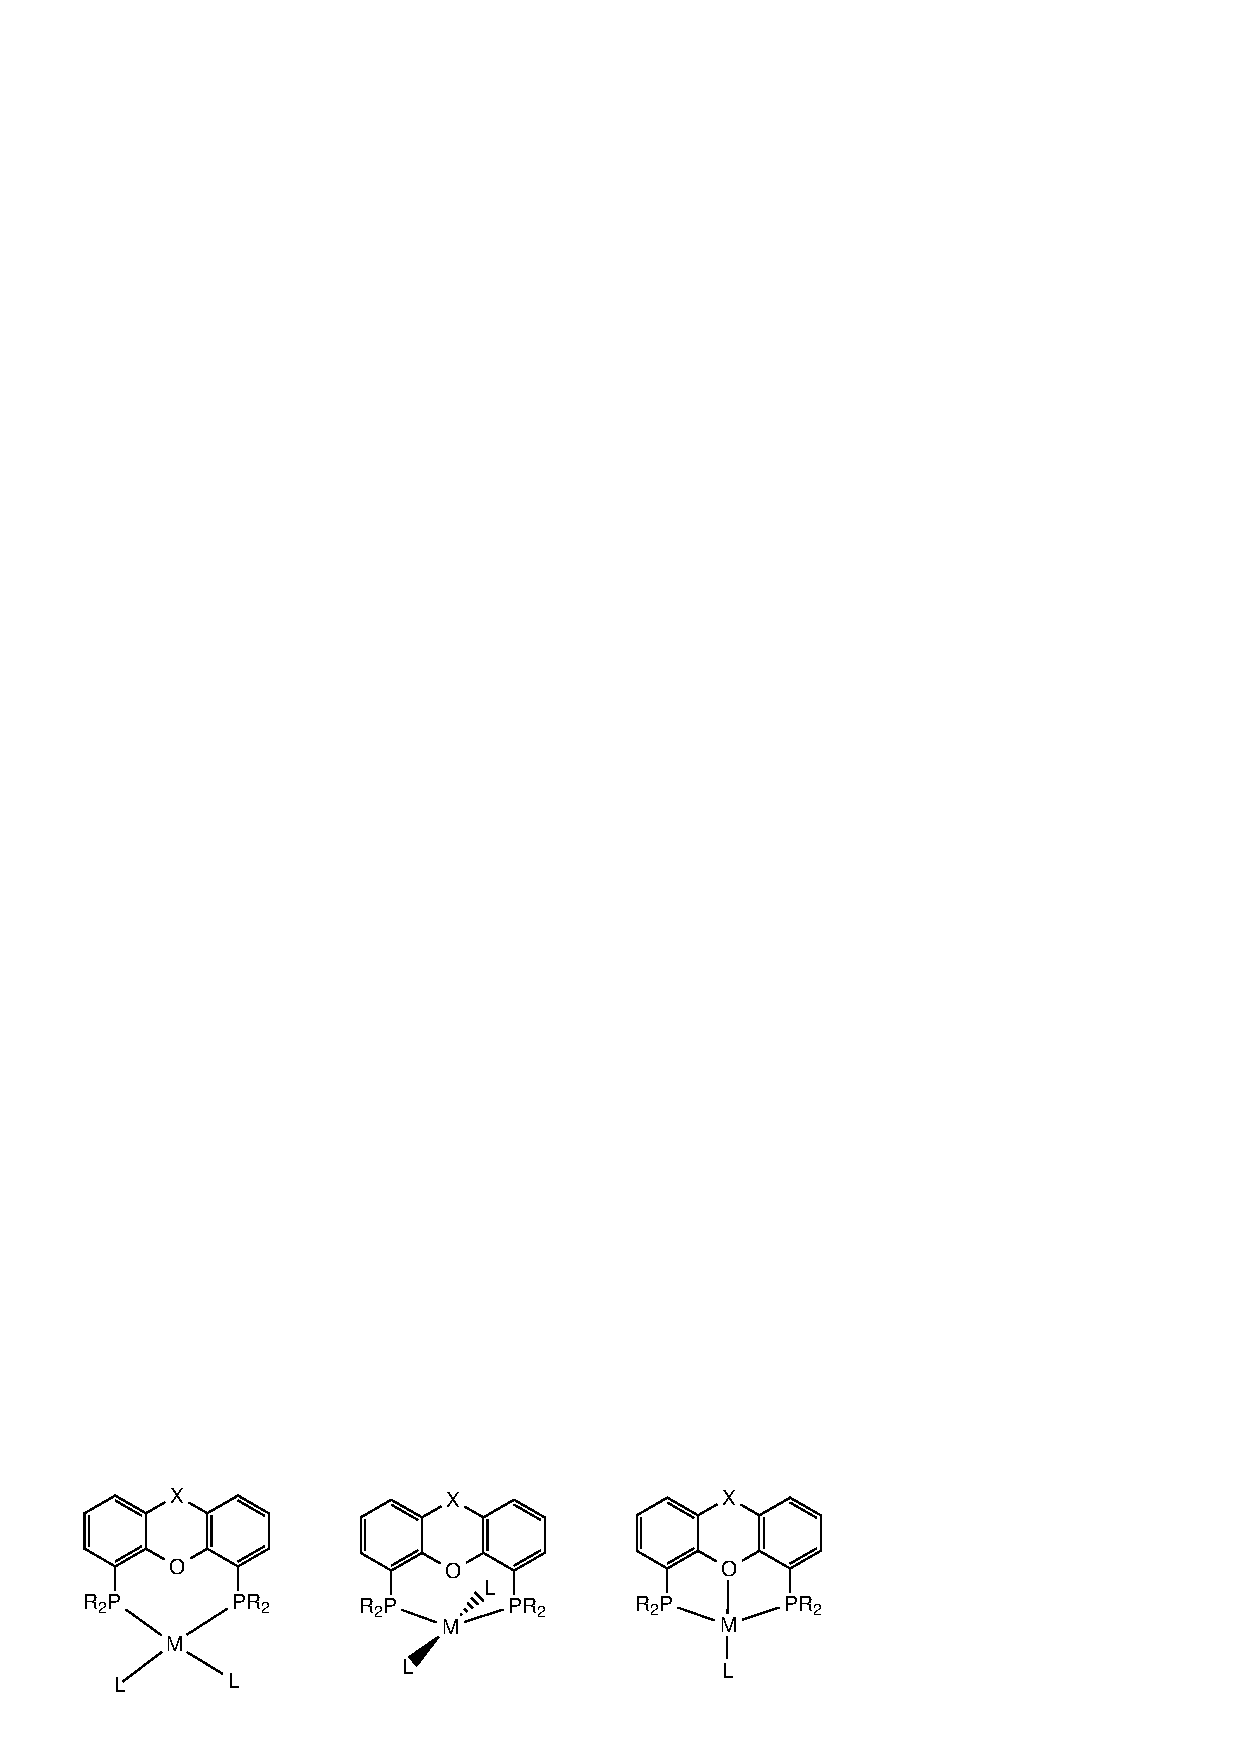
\includegraphics[width = 0.5\textwidth]{../Figures/Bondingmodes.pdf}
\caption[Bonding in organometallic complexes]{Bonding in organometallic complexes}
\label{Bondingmodes}
\end{figure}

Alkanes are weak $\sigma$-bases and $\pi$-acids.  As such they are very poor ligands for transition metals.\cite{Crabtree1993}  Typically alkanes form $\sigma$-complexes with metals that can $\pi$-backbond.  For successful complexation a low valent metal and the absence of competitive decomposition pathways are required.\cite{Crabtree2001}  Enhanced bonding of alkanes occurs with metals capable of forming enhanced $\pi$-backbonding into the $\sigma$* C-H orbital, similar to that found for molecular hydrogen complexes.\cite{Kubas1988}

The activation of C-H bonds is thought occur \emph{via} a stepwise process involving the coordination of the alkane to the metal to form a $\sigma$-complex, followed by the oxidative cleavage of the C-H bond forming metal-alkyl and metal-hydride bonds.\cite{Labinger2002}  The intermediate  $\sigma$-complexes are highly unstable and until recently their existence had only been inferred by isotope scrambling and the inverse kinetic isotope effect in reductive elimination reactions of alkyl hydrides.\cite{Bernskoetter2009, Labinger2002}  In 2009 Brookhart reported the characterisation of a relatively long-lived rhodium(I) $\sigma$-methane complex.\cite{Bernskoetter2009}  The complex was formed by the protonation of a rhodium methyl complex (Scheme \ref{Sigmamethane}).  At -87~\degrees C the methane is displaced by solvent (\ce{CDCl2F}) with a half-life of 83 minutes.

\begin{scheme}[h]
\centering
\includegraphics[]{../Schemes/Sigmamethane.pdf}
\caption[Formation of a $\sigma$-methane complex]{Formation of a $\sigma$-methane complex.  Ar\ce{^{F}} = \emph{m}-di(trifluoromethyl)phenyl}
\label{Sigmamethane}
\end{scheme}

%$\sigma$-Complexes of methane have been proposed 
%The first example of C-H activation was reported by Dimroth in 1902\cite{Dimroth1902}  Reaction of phenol with a solution of mercury acetate on a steam bath replaced the \emph{ortho} and \emph{para}-protons with a mercury acetate group.  \fixme{more info etc}

C-H activation has developed significantly since the first example of C-H activation by an organometallic complex was reported by Chatt in 1962. \cite{Chatt1962}  Reduction of metal halides by sodium napthalene in the presence of an excess of \gls{dmpe} produced V, Cr, Mo and W complexes of the form \ce{[M(}\gls{dmpe}\ce{)_3]},  and Fe and Co complexes of the form \ce{[M(}\gls{dmpe}\ce{)_2]}.  However, the \ce{[Ru(}\gls{dmpe}\ce{)_2]} analogue gave a hydride complex ``by taking hydrogen from the napthalene.''\cite{Chatt1962}  

Further analysis of the ruthenium system was carried out and published in 1965.\cite{Chatt1965} Reaction of \emph{cis}- or \emph{trans}-\ce{[RuCl2(}\gls{dmpe}\ce{)_2]} with benzene, naphthalene, anthracene and phenylanthracene formed the \emph{cis}-\ce{[RuH(aryl)(}\gls{dmpe}\ce{)_2]} (aryl = phenyl, naphthyl, anthryl and phenanthryl) complexes \emph{via} oxidative addition.\cite{Chatt1965}  The activation is reversible, as reactions of the complexes with hydrochloric acid yielded hydrogen gas, the aromatic starting material and \emph{cis}-\ce{[RuCl2(}\gls{dmpe}\ce{)_2]} (Equation \ref{ChattCH}).  The C-H activation to form the complexes was selective for example, in the reaction with naphthalene the activation occurred exclusively at the 2-position.

\vspace{-0.6 cm}
\begin{equation}
\ce{[RuH(C10H7)(dmpe)2] + 2HCl} \longrightarrow \ce{[RuCl2(dmpe)2] + H2 + C10H8}
\label{ChattCH}
\end{equation}

The naphthyl hydride complex formed by treatment of \ce{[Ru(}\gls{dmpe}\ce{)_2]} with naphthalene thermally decomposed giving a complex with properties consistent with \ce{[Ru(}\gls{dmpe}\ce{)_2]} (Scheme \ref{Chattdmpescheme}).\cite{Chatt1965}  However, infrared spectroscopy showed a signal for a Ru-H at 1791 \percm,  leading to the proposed structure of \ce{[RuH(CH2PMeCH2CH2PMe2)(}\gls{dmpe})], formed by activation of a C-H bond from the \gls{dmpe} ligand.\cite{Chatt1965}  X-ray crystallography later allowed the reformulation of the structure to the analogous dimer.\cite{Crabtree2004}  However, this species remains the first example of cyclometallation of an sp$^3$ C-H bond.

\begin{scheme}[h]
\centering
\includegraphics[]{../Schemes/Chattdmpescheme.pdf}
\caption[C-H activation reactions reported by Chatt and Davidson]{C-H activation reactions reported by Chatt and Davidson\cite{Chatt1965}}
\label{Chattdmpescheme}
\end{scheme}

The exchange of hydrogen with deuterium in polyalkyl benzenes, polycyclic aromatic hydrocarbons and heterocycles can be catalysed by homogeneous platinum (II) species.\cite{Hodges1968, Hodges1969, Hodges1969b}  Using deutero-acetic acid as a solution in \ce{D2O}, together with DCl or anhydrous tin(IV) chloride to prevent the formation of platinum metal, H/D exchange on the substrate was observed when exposed to \ce{Na2PtCl4} or \ce{K2PtCl4}.\cite{Hodges1968, Hodges1969}  Although the rate of exchange was faster for unhindered aromatic protons, H/D exchange was also observed for alkyl protons.\cite{Hodges1969b}  The rate was fastest for \hbox{\emph{p}-xylene}, \gls{mesitylene}, \emph{m}-xylene and toluene, however exchange of alkyl protons was also observed in \emph{o}-xylene, \gls{hemimellitene} and \gls{durene}.\cite{Hodges1969b}

This activation of alkyl protons inspired Shilov to investigate the C-H activation of alkanes by platinum.  The system carries out oxidation of alkanes such as methane \emph{via} electrophilic activation (Scheme \ref{Shilovcatalyticcycle}).\cite{Labinger2002, Crabtree2001}  The first step involves displacement of a chloride ligand on the platinum by a $\sigma$-methyl followed by oxidative addition and loss  of H$^+$ \emph{via} loss of HCl.  The Pt(II) is then  oxidised to Pt(IV) \emph{via} electron transfer to the \ce{PtCl6}$^{2-}$.  Finally, the complexed methyl undergoes nucleophilic attack from water displacing the \emph{trans} chloride ion to form HCl, methanol and regenerate the catalyst.  The system has shown selectivity for terminal C-H bonds.  For example, in the oxidation of ethanol functionalisation occurs at the methyl to yield ethylene glycol (Equation \ref{Ethyleneglycol}) whilst, all other methods of oxidation will oxidise the hydroxyl functionality.\cite{Labinger1993}  This can be utilised for the one-pot synthesis of ethylene glycol from ethanol.\cite{Sen1994}  However, the selectivity is lost in reaction with 2-propanol which gives only acetone.\cite{Labinger1993}
\vspace{-1.5cm}
\begin{scheme}[h]
\centering
\includegraphics[]{../Schemes/Shilovcatalyticcycle.pdf}
\caption[Platinum catalysed oxidation of alkanes]{Platinum catalysed oxidation of alkanes}
\label{Shilovcatalyticcycle}
\end{scheme}

\begin{equation}
\ce{CH3CH2OH + H2O + PtCl6}^{2-} \longrightarrow \ce{CH2OHCH2OH + PtCl4}^{2-} + \ce{2HCl} 
\label{Ethyleneglycol}
\end{equation}

Although the Shilov system is catalytic in Pt(II), it requires a stoichiometric amount of Pt(IV).  In addition, the Pt(II) catalyst is unstable in solution and eventually precipitates as platinum metal.\cite{Luinstra1995}  This results in an expensive and thus impractical system for industrial application.  The relatively low yields of the system also reduce its industrial viability.\cite{Periana1993}  Furthermore, the reaction produces two equivalents of hydrochloric acid which require disposal at significant cost.\cite{Poliakoff2001}  A number of attempts have been made to replace the Pt(IV) primary oxidant thus making an economically viable system.\cite{Periana1993, Periana1998, Hashiguchi2010}  However, this has proven challenging as most oxidants tend to convert Pt(II) to the inactive Pt(IV).\cite{Crabtree2001}  Additionally, an oxidant is required that will not attack the product alcohol.  

In 1993 Periana reported the use of concentrated sulfuric acid as the primary oxidant and Hg(II) as a catalyst in place of the platinum.\cite{Periana1993}  The Hg(II) is the highest possible oxidation state so further unwanted oxidation of the catalyst is not possible.  Using methane as the feedstock, the system produces methyl bisulfate in a 43\% yield (Scheme \ref{Mercurycatalyticcycle}).  This has the advantage of being highly resistant to oxidation preventing the formation of carbon dioxide. However, the catalysis involves the formation of MeHg(II)$^+$ as an intermediate following activation.  Methyl mercury salts, like most organomercury compounds, are extremely toxic and exhibit accumulation effects in biological systems.\fixme{cite(MethylmercuryMSDS)}  Sulfur dioxide, a significant contributor to acid rain,\cite{Jacobs1999} is also produced as a stoichiometric byproduct of this reaction.  However, the oxidation of sulfur dioxide to sulfuric acid by air is an established industrial process and could be utilised to provide further sulfuric acid for the process.\cite{Periana1993}

%\begin{equation}
%\ce{CH4 + 2H2SO4} \longrightarrow \ce{CH3OSO3H + 2H2O + SO2} 
%\label{Mercuryequation}
%\end{equation}

%Periana 1993 reaction is carried out at 180 degrees
%Periana 1998 reaction is carried out at 100 degrees

\begin{scheme}[h]
\centering
\includegraphics[width = 0.8\textwidth]{../Schemes/Mercurycatalyticcycle.pdf}
\caption[Mercury catalysed oxidation of methane]{Mercury catalysed oxidation of methane}
\label{Mercurycatalyticcycle}
\end{scheme}

Further work by Periana investigated changing the Pt(II) system to improve stability, activity and prevent oxidation to Pt(IV).\cite{Periana1998}  Nitrogen donor ligands were utilised as oxygen systems have high kinetic lability on platinum and phosphorus ligands have poor oxidative and thermal stability.  The use of \emph{cis}- or \emph{trans}-\ce{[PtCl2(NH3)2]} in concentrated sulfuric acid at 180~\degrees C gave 90\% selectivity for methyl bisulfate.  However, the catalyst degraded to insoluble \ce{PtCl2} and \ce{NH4HSO4}.  

In an extension of this work a $\pi$-acidic chelating donor ligand \gls{bpym} was utilised as $\pi$-donor ligands were expected to have lower proton affinity and form stronger Pt-N bonds than the \ce{NH3} ligands used previously.  The \ce{[PtCl2(}\gls{bpym})] complex was tested in 20 \% \ce{SO3} in \ce{H2SO4} at 200~\degrees C for 50 hours.  Some free ligand and HCl was observed, however the solution remained homogenous showing no formation of platinum metal or other insoluble products.  Using \emph{cis}-\ce{[PtCl2(}\gls{bpym})] in the catalytic system at 220~\degrees C for 2.5 hours resulted in 90\% methane conversion with an 81\% selectivity (carbon dioxide forming the major byproduct).\cite{Periana1998}  However, this reaction requires high temperatures and forms significant amounts of carbon dioxide and sulfur dioxide both of which are environmentally hazardous.\cite{Jacobs1999}  The reaction proceeds \emph{via} a slightly different mechanism to the mercury system (Scheme \ref{PerianaPtcycle}) with oxidation occurring prior to the functionalisation.\cite{Periana1998}

%\begin{figure}[h]
%\centering
%\includegraphics[height = 4cm]{../Figures/bpym.pdf}
%\caption[Structure of \ce{[PtCl2(bpym)]}]{Structure of \ce{[PtCl2(bpym)]}}
%\label{bpym}
%\end{figure}

\begin{scheme}[h]
\centering
\includegraphics[width = 0.9\textwidth]{../Schemes/PerianaPtcycle.pdf}
\caption[Oxidation of methane catalysed by \ce{[PtCl2(bpym)]}]{Oxidation of methane catalysed by \ce{[PtCl2(bpym)]}}
\label{PerianaPtcycle}
\end{scheme}

%Nature of the C-H bond\\ 
%Strong\\
%Highly non-polar\\
%General catalytic attempts\\
%Shilov etc.\\

\subsection{Alkane dehydrogenation}

Alkane dehydrogenation is an alternative approach that combines the activation and functionalisation into a single step.  This methodology was developed from the \hbox{organometallic} complexes such as Wilkinson's\cite{Osborn1966} and Crabtree's\cite{Crabtree1979b} catalysts (Figure \ref{Wilkinsoncrabtree}) that are utilised as homogeneous hydrogenation catalysts.  Wilkinson's catalyst was the first homogeneous hydrogenation catalyst with comparable rates to the heterogeneous counterparts and has become very widely utilised in organic synthesis.\cite{Knowles2003}

\begin{figure}[h]
\centering
\includegraphics[]{../Figures/Wilkinsoncrabtree.pdf}
\caption[Wilkinson's and Crabtree's catalysts]{Wilkinson's (a) and Crabtree's (b) catalysts}
\label{Wilkinsoncrabtree}
\end{figure}

Crabtree reported a number of hydrogenation catalysts based on Wilkinson's catalyst in 1977.\cite{Crabtree1977} The most active of these, \ce{[Ir(cod)(PCy3)(py)]PF6} (Figure \ref{Wilkinsoncrabtree} b, \gls{cod} = 1,5-cyclooctadiene, \gls{Cy}~=~cyclohexyl, \gls{py} = pyridyl) has become known as Crabtree's catalyst.\cite{Cui2005}  This catalyst is active for the hydrogenation of a range of \hbox{mono-,} di-, \hbox{tri-,} and \hbox{tetra-substituted} alkenes with turnover frequencies (\glspl{TOF}) of 6400, 4500, 3800 and 4000 for hex-1-ene, cyclohexene, 1-methylcyclohexene and 2,3-dimethylbut-2-ene respectively.\cite{Crabtree1979b}  Crabtree's catalyst is useful for the hydrogenation of tri- and tetra-substituted alkenes for which Wilkinson's catalyst is inactive.\cite{Cui2005}

A catalytic system lowers the activation energy for a reaction, hence both the forward and reverse reactions will be catalysed.\cite{Crabtree2001}  This realisation led Crabtree to test an iridium system for dehydrogenation of alkenes.\cite{Crabtree1979}  The dehydrogenation would normally be strongly endothermic so the substrates were chosen to give products that would bind strongly to the metal to improve the thermodynamics of the reaction.  In the presence of \ce{[IrH2(alkene)2(PPh3)2]+} and 3,3-dimethylbut-1-ene (as hydrogen acceptor) the dehydrogenation of cyclooctene, [2.2.2]bicyclooctene, cyclopentene and cyclohexene were carried out successfully to give complexes of the type \ce{[Ir(diene)(PPh3)2]+} and \ce{[Ir(Cp)H(PPh3)]+} (Cp = cyclopentadienyl).\cite{Crabtree1979}  The dehydrogenation of alkanes was also possible with the system.  The dehydrogenation of cyclopentane to form the cyclopentadienyl complex gave a 30\% yield after 18 hours, whilst the dehydrogenation of cyclooctane to the cyclooctadiene complex gave a 70\% yield after only 4 hours.\cite{Crabtree1979}

Felkin reported a rhenium complex capable of dehydrogenating linear alkanes to dienes.\cite{Baudry1982}  In the presence of \ce{[ReH7(PAr3)2]} (Ar = \emph{p}-\ce{MeC6H4}) and 3,3-dimethylbut-1-ene, \emph{n}-pentane was dehydrogenated to form a diene complex (Scheme \ref{Pentanedehydrogenation}).  Treatment of this complex with \ce{P(OMe)3} produced pent-1-ene with a yield of 45\%.  This was extended to the linear isomers of hexane, heptane and octane.\cite{Baudry1984}  Although pentane can form only one conjugated diene complex, hexane and heptane can give two, whilst octane can give three.  However, in all cases upon treatment of the complex with \ce{P(OMe)3} the terminal alkene was formed with a selectivity of over 95\%.\cite{Baudry1984}  

\begin{scheme}[h]
\centering
\includegraphics[]{../Schemes/Pentanedehydrogenation.pdf}
\caption[Dehydrogenation of pentane]{Dehydrogenation of pentane reproduced from Felkin et al.\cite{Baudry1982}}
\label{Pentanedehydrogenation}
\end{scheme}

Wilkinson's catalyst (figure \ref{Wilkinsoncrabtree}b) has also been utilised as a dehydrogenation catalyst.\cite{Fujii1990}  The dehydrogenation of cyclooctane to give cyclooctene by \ce{[RhCl(L)3]} (L = \ce{PPh3} or P(\emph{p}-\ce{tolyl)3}) was carried out at reflux (151~\degrees C) without the need for a hydrogen acceptor.  The high temperature of the reaction mixture is sufficient to allow the removal of molecular hydrogen from the reaction mixture.\cite{Fujii1990}  The reaction rates obtained with this system were low, the highest with L = P(\emph{p}-\ce{tolyl)3} was only 1.24 h\ce{^{-1}} with a L/Rh ratio of 8.\cite{Fujii1990}

Crabtree utilised this acceptorless methodology to test the catalytic activity of iridium complexes.\cite{Aoki1993}  \ce{[IrH2L(PCy3)2]} (L = \ce{O2CCF3}, \ce{O2CC2F5} and \ce{O2CPhCH2}) were active for the dehydrogenation of cyclooctane under reflux with initial turnover frequencies of 1.41, 1.05 and 0.22 \ce{h^{-1}} respectively.  However, the complexes were unstable with deactivation half lives of 15, 34 and 14 hours respectively.\cite{Aoki1993}  Alternate methods to remove the hydrogen were also tested.  Using perfluorodecalin as a solvent allowed for more effective hydrogen removal due to the higher volatility compared to cyclooctane.  This resulted in poor activity with a turnover frequency of 0.24 \ce{h^{-1}} using \ce{[IrH2(O2CCF3)(PCy3)2]} as catalyst.  Bubbling inert gas was unsuccessful with cyclooctane as a substrate as a large amount of the substrate was lost.  However, using the less volatile cyclodecane a turnover frequency of 0.48 \ce{h^{-1}}  was obtained.\cite{Aoki1993}

%\fixme{Goldman reference 4 from Gupta1996 had an improved non-pincer system}

\section{Pincer ligands}

Recently, the so-called pincer ligands have attracted a great deal of research attention due to their unique balance of stability and reactivity.\cite{Becerra2009}  Pincer ligands are tridentate ligands that bind in a meridional fashion, examples of which are given in Figure \ref{Pincernaming}.  Pincer ligands are named based on their donor atoms such as, PCP, NCN, and POP.  If the groups between the donor atoms contain heteroatoms then these may be included in the naming also, for example POCOP.  The pincer ligands may be anionic (as with PCP ligands) or neutral (PNP and POP).\cite{Vlugt2009, Kataoka1995}  Although phosphines are the most common donor groups, amines,\cite{Singleton2003} imines,\cite{Takenaka2005} thioethers\cite{Zim2000} and N-heterocyclic carbenes\cite{Hahn2007} have all been reported.

\begin{figure}[h]
\centering
\includegraphics[]{../Figures/Pincernaming.pdf}
\caption[Naming of pincer ligands]{Naming of pincer ligands}
\label{Pincernaming}
\end{figure}

The first reports of pincer ligands were in 1976 by Shaw\cite{Moulton1976} and Alcock.\cite{Alcock1976}  Shaw reported a \emph{tert}-butyl PCP ligand (Figure \ref{Shaw}) and introduced the naming scheme that has become commonplace for pincer ligands.  When reacted with an appropriate metal precursor, complexes formed between the tridentate ligand with nickel, palladium, platinum, rhodium and iridium with chloride, nitrile, hydride and carbon monoxide ligands.\cite{Moulton1976} 

\begin{figure}[h]
\centering
\includegraphics[]{../Figures/Shaw.pdf}
\caption[First reported PCP pincer ligand]{First reported PCP pincer ligand}
\label{Shaw}
\end{figure}

Alcock reported X-ray crystal structures of the first complexes of POP ligands (Figure \ref{Alcock}).\cite{Alcock1976}  These formed rhodium carbonyl complexes that were characterised by X-ray crystallography.  With a single ether group in the backbone it forms a typical pincer complex, bonding through the phosphorus and oxygen atoms.  However, when there are three ether units the phosphorus atoms bond to the rhodium but the oxygen H-bonds to a water molecule that is bound to the rhodium centre.\cite{Alcock1976}

\begin{figure}[h]
\centering
\includegraphics[]{../Figures/Alcock.pdf}
\caption[First reported POP pincer ligand]{First reported POP pincer ligand}
\label{Alcock}
\end{figure}

%Typically the central donor atom E is a carbon from an aromatic ring that binds through C-H activation to form a metallacycle.\cite{Choi2011}  

The different components of pincer ligands have significant influence on the steric and electronic properties and hence their reactivity.\cite{Singleton2003}  Altering the group X (Figure \ref{Pincerligands}) can lead to significant electronic effects mostly through the \emph{trans} influence.\cite{Choi2011}  For example, a carbon donor ligand has a greater \emph{trans} influence than an oxygen donor, so ligands \emph{trans} to X in PXP complexes will be bound more strongly when X~=~O than X~=~C.\cite{Zhu2008} The donor group Y controls the steric environment around the metal centre and the electron density.\cite{Choi2011}  Changing the backbone and other remote groups gives control over the electron density on the metal and can be used to improve solubility properties.\cite{Choi2011}

\begin{figure}[h]
\centering
\includegraphics[]{../Figures/Pincerligands.pdf}
\caption[General representation of pincer ligands]{General representation of pincer ligands}
\label{Pincerligands}
\end{figure}

The tridentate coordination of pincer ligands, typically forming two five-membered metallacycles, imparts significant stability to metal complexes with pincer ligands.\cite{Choi2011}  The stability of the complexes is such that the backbone can undergo functionalisation at the 4-position to trimethylsilane \emph{via} lithiation with \emph{tert}-butyllithium and treatment with trimethylchlorosilane without inducing any decomposition of the platinum complex (Scheme \ref{Stability}).\cite{Albrecht2001}  This inherent stability allows the complexes to act as catalysts for highly endothermic reactions that require high temperatures, such as alkane dehydrogenation.\cite{Choi2011}

\begin{scheme}[h]
\centering
\includegraphics[]{../Schemes/Stability.pdf}
\caption[Functionalisation of an NCN pincer ligand]{Functionalisation of an NCN pincer ligand}
\label{Stability}
\end{scheme}

Coordination complexes of pincer ligands have a large number of applications.  Platinum complexes of an NCN pincer ligand have been utilised as sensors for the detection of sulfur dioxide.\cite{Albrecht2000, Albrecht2000c, Albrecht2001}  Palladium and nickel complexes of a number of pincer ligands have shown activity in cross-coupling reactions.\cite{Hahn2007, Bedford2000, Kimura2006, Zim2000, Obora2006} Theoretical studies have shown potential uses for pincer ligands in water-splitting\cite{Sandhya2011} and nitrogen fixation.\cite{Holscher2007}  However, one of the most prominent uses of pincer ligands is the activation of C-H bonds, typically as dehydrogenation catalysts.\cite{Choi2011, Albrecht2001, Crabtree2001}

%\subsection{Gas sensors}

%Platinum complexes of an NCN pincer (Figure \ref{Gassensors} \fixme{reference the structure correctly}) have been studied in solution or the crystalline state for use in the detection of sulfur dioxide.\cite{Albrecht2000, Albrecht2000c, Albrecht2001b}  In the presence of sulfur dioxide the square planar complex rapidly (less than 50 \si{\micro\second} adsorb the gas to form square pyramidal structures.\cite{Albrecht2000}  The adsorption is accompanied by a dramatic colour change from colourless to bright orange and is reversible upon exposure to a sulfur dioxide free atmosphere.\cite{Albrecht2000}  Dendrimer derivatives (2 and 3, Figure \ref{Gassensors}) can be used to detect sulfur dioxide at concentrations as low as 5 ppm (in a nitrogen atmosphere) \cite{Albrecht2001b}  

%\begin{figure}[h]
%\centering
%\includegraphics[width = \textwidth]{../Figures/Gassensors.pdf}
%\caption[NCN platinum complexes used for sensing \ce{SO2}]{NCN platinum complexes used for sensing \ce{SO2}}
%\label{Gassensors}
%\end{figure}

%These sensors have been studied further for physiological applications.  The complex (Figure \ref{Physiologicalgassensors}) is stable in both acidic and basic aqueous solutions for prolonged periods.\cite{Albrecht2000b}  Testing in conditions known to lead to rapid protein degradation (pH < 1, 50 \degrees C, 5 hours) results in no detectable decomposition.\cite{Albrecht2000b}  The coordination of sulfur dioxide to the complex results in a large shift in the $^{195}$Pt NMR of 1150 ppm (from -3150 to -2000 ppm).\cite{Albrecht2000b}  This could be detected by MRI for medical applications.  These complexes are also being developed for use as molecular switches for opto-electronics.\cite{Albrecht2000c}

%\begin{figure}[h]
%\centering
%\includegraphics[height = 4.5cm]{../Figures/Physiologicalgassensors.pdf}
%\caption[NCN platinum complexes developed for \ce{SO2} sensing in physiological settings]{NCN platinum complexes developed for \ce{SO2} sensing in physiological settings}
%\label{Physiologicalgassensors}
%\end{figure}

%\subsection{Cross-coupling reactions}

%Coordination complexes of pincer ligands also find use as catalysts in carbon-carbon cross-coupling reactions such as the Suzuki, Heck \fixme{etc}.

%Pincer ligands with N-heterocyclic carbene (NHC) donors are becoming more common.\fixme{reference}  The palladium complexes found in figure \ref{CCCPincers} are active for the heck cross-coupling reaction of aryl bromides with styrene and the suzuki cross-coupling of aryl bromides with phenylboronic acid.\cite{Hahn2007}  Using a 1 mol \% catalyst loading the reaction of 4-bromobenzaldehyde and 4-bromoacetophenone with styrene quantitative yields were obtained after 24 hours regardless of the substituent on the ligand.  Using the \emph{n}-butyl derivatised ligand after two hours yields of 84.1, and 60.0 \% were obtained for reaction of styrene with 4-bromobenzaldehyde and 4-bromoacetophenone respectively.   The \emph{n}-butyl derived ligand formed an active palladium catalyst for the Suzuki cross-coupling of phenylboronic acid with 4-bromobenzaldehyde and 4-bromoacetophenone.  Using a 0.1 \% catalyst loading  yields of 50.7 and 48.7 \% respectively were obtained after two hours and quantitative conversion obtained in 24 hours.

%\begin{figure}[h]
%\centering
%\includegraphics[height = 6 cm]{../Figures/CCCPincers.pdf}
%\caption[Palladium complexes with NHC donor pincer ligands]{Palladium complexes with NHC donor pincer ligands}
%\label{CCCPincers}
%\end{figure}

%The palladium complexes with ferrocene based PCP ligands (figure \ref{Ferrocenepalladium}) have been tested for activity in the Suzuki cross-coupling reaction.\cite{Sheloumov2008}  After 4.5 hours the reaction of 4-bromoacetophenone with phenylboronic acid in the presence of 1 and 3 was almost complete with 84 and 84.5 \% yields respectively under homogeneous conditions and quantitative yields under biphasic conditions (decane/\ce{H2O}).  The reaction was much slower with complex 2 with only 66 \% obtained after 15 hours.  Similar activities for all complexes were obtained for the homogeneous reaction of phenylboronic acid with 4-bromoanisole with yields of 77, 79 and 98 \% after 12, 15 and 15.5 hours for 1, 2 and 3 respectively.  However under biphasic conditions complex 2 was much less reactive obtaining a yield of 9 \% after 15 hours compared to 62 and 63.5 \% for 1 and 3 respectively.  The lower activity for complex 2 is thought to be due to the steric bulk of the \emph{tert}-butyl groups though in complex 3 the steric effect is overcome by the electronic influence of the Fe(III) rather than Fe(II).\cite{Sheloumov2008}

%See 

%\begin{figure}[h]
%\centering
%\includegraphics[height = 4.5cm]{../Figures/Ferrocenepalladium.pdf}
% \caption[Palladium complexes of ferrocene pincer ligands]{Palladium complexes of ferrocene pincer ligands}
%\label{Ferrocenepalladium}
%\end{figure}

%Definition\\	
%Naming\\
%Uses of the ligands\\
%Gas sensors\\
%SO2\\
%PCP\\
%POCOP\\
%PNP\\
%POP\\
%Nitrogen activation and fixation\\

\subsection{C-H activation}
%\subsection{Alkane dehydrogenation}

The catalytic dehydrogenation of alkanes has the potential to develop into an important industrial process allowing alkanes to be used as a chemical feedstock, without requiring high temperature cracking or other inefficient processes.\cite{Choi2011}  The first use of pincer complexes for alkane dehydrogenation was reported by Gupta in 1996.\cite{Gupta1996}  The rhodium and iridium dihydride complexes in figure \ref{Dehydrogenationligands} were tested for the dehydrogenation of cyclooctane in the presence of 3,3-dimethylbut-1-ene as hydrogen acceptor.  Rates of 0.8 turnovers h$^{-1}$ at 150~\degrees C were obtained for the rhodium complex, whilst the iridium complex was more active with rates of 82 turnovers h$^{-1}$.\cite{Gupta1996}  The catalysts used were highly stable at this temperature for extended periods and the addition of mercury did not inhibit the reaction indicating a homogeneous system.\cite{Gupta1996}  The higher activity of the iridium complex combined with the high thermal stability has led to a focus on iridium complexes for alkane dehydrogenation.\cite{Choi2011}

\begin{figure}[h]
\centering
\includegraphics[]{../Figures/Dehydrogenationligands.pdf}
\caption[Rhodium and iridium pincer complexes used for alkane dehydrogenation]{Rhodium and iridium pincer complexes used for alkane dehydrogenation}
\label{Dehydrogenationligands}
\end{figure}

The iridium complex (Figure \ref{Dehydrogenationligands}) was also active for the dehydrogenation of cyclic alkanes, tetrahydrofuran and ethylbenzene to give arenes, furan and styrene respectively.\cite{Gupta1997, Gupta1997b}  In all cases the presence of excess 3,3-dimethylbut-1-ene as hydrogen acceptor inhibited the reaction so it was necessary to add this periodically.  A nitrogen atmosphere also inhibited reaction indicating competitive binding of nitrogen and alkane to the active site.\cite{Gupta1996, Gupta1997, Gupta1997b}  The iridium complex is also active for the dehydrogenation of cyclooctane and cyclodecane under acceptorless conditions.\cite{Xu1997}  A solution of fresh catalyst could be poisoned by addition of 10\% alkene rendering the catalyst inactive and indicating that the reduction of activity over time is not due to catalyst decomposition.\cite{Xu1997}

A mechanism for the alkane transfer dehydrogenation (Scheme \ref{Dehydrogenationcatalyticcycle}) has been elucidated \emph{via} a kinetics study by Goldman.\cite{Renkema2003}  The 3,3-dimethylbut-1-ene inserts into an iridium hydride bond, which is followed by reductive elimination to give the alkane.  The substrate undergoes oxidative addition to the iridium centre, which is followed by $\beta$-hydride elimination to give the alkene product and regenerate the iridium-dihydride.  With a limited concentration of 3,3-dimethylbut-1-ene (as is typical for these reactions) the rate determining step is the hydrogenation of the acceptor rather than C-H activation of the alkane, however with an excess of acceptor the rate determing step is the reaction with the cyclooctane.\cite{Renkema2003}  

\begin{scheme}[h]
\centering
\includegraphics[]{../Schemes/Dehydrogenationcatalyticcycle.pdf}
\caption[Proposed mechanism for transfer dehydrogenation]{Proposed mechanism for transfer dehydrogenation}
\label{Dehydrogenationcatalyticcycle}
\end{scheme}

The three-coordinate [Ir(PCP)] intermediate formed following C-H elimination (Figure \ref{Dehydrogenationcatalyticcycle}) was proposed on the basis of an NMR study showing that the dihydride complex will react with 3,3-dimethylbut-1-ene to give the \emph{trans}-2-(\emph{tert}-butyl)vinyl complex that is in equilibrium with [Ir(PCP)] on an NMR timescale.\cite{Kanzelberger2000}  A more recent study has reported this resting state of the complex as the $\pi$-alkene complex and it is likely that both occur depending on the concentration of the hydrogen acceptor.\cite{Choi2011}  Studies into the acceptorless reaction have shown a similar mechanism.\cite{Krogh2002, Krogh2002b}  In this case the rate determining step is the thermolytic loss of \ce{H2} to give the active dehydrogenation complex [Ir(PCP)].  The inhibition of activity resulting from a build-up of alkene is likely due to the formation of the $\pi$-alkene complex and increased rate of the reverse reaction.\cite{Krogh2002, Krogh2002b}

Introduction of electron-donating groups such as \ce{OCH3} in the \emph{para}-position (Figure \ref{DFTpincers}) was shown to favour oxidative addition of an alkane to the 14-electron [Ir(PCP)] complex whilst disfavouring further addition of alkane to the \ce{[(PCP)Ir(R)(H)]} complex.\cite{Krogh2002c}  In the acceptorless dehydrogenation of cyclodecane at reflux (201 \degrees C) the electron-donating \ce{OCH3} pincer complex achieved 820 turnovers in 48 hours compared to 360 with a hydrogen in the \emph{para}-position.\cite{Zhu2004}   However, in dehydrogenation of \emph{n}-undecane at 196 \degrees C little difference was seen between the H and \ce{OCH3} substituted ligands with turnovers of 76 and 91 respectively after 4 hours.  The less sterically bulky isopropyl derivative (with \ce{OCH3} in the \emph{para}-position) was also tested and achieved 2970 turnovers over 48 hours for the dehydrogenation of cyclodecane, indicating that the steric bulk of the ligand has a significant influence of the rate of reaction.\cite{Zhu2004}   In the dehydrogenation of \emph{n}-undecane at 196~\degrees C the isopropyl catalyst was much less active than the \emph{tert}-butyl with only 30 turnovers achieved after 4 hours.  	

\begin{figure}[h]
\centering
\includegraphics[]{../Figures/DFTpincers.pdf}
\caption[Electron-donating pincer ligands]{Electron-donating pincer ligands}
\label{DFTpincers}
\end{figure}

The steric environment imposed by the pincer ligand has a significant impact on the activity towards alkane dehydrogenation.\cite{Choi2011}  A computational and experimental study into this effect was reported by Brookhart in 2009.\cite{Kundu2009}  By exchanging the \emph{tert}-butyl groups on the xylene based PCP complex for methyl groups the impact of the sterically bulky \emph{tert}-butyl groups on alkane dehydrogenation could be studied.  Exchanging a single \emph{tert}-butyl results in a decrease in the transition state for the rate determining step ($\beta$-H elimination) of 42 kJmol$^{-1}$.  This was offset slightly by an increase of 17 kJmol$^{-1}$ in the bond strength of but-1-ene to the iridium centre.  Exchanging a second \emph{tert}-butyl for a methyl was calculated to have a much smaller overall impact as the but-1-ene bonds much more strongly to the metal centre.\cite{Kundu2009}  These results were supported experimentally in the transfer dehydrogenation of \emph{n}-octane using 3,3-dimethylbut-1-ene as the acceptor.  With one and two methyls replacing \emph{tert}-butyl groups, 195 and 140 turnovers were obtained respectively, compared to only 53 for the unmodified ligand.\cite{Kundu2009}

Although the PCP iridium complexes are stable at 150 \degrees C for extended periods, significant decomposition becomes apparent after 24 hours at 200 \degrees C.\cite{Gupta1996}  Ligands based on an anthracene backbone (Figure \ref{Anthraphos}) were developed to achieve a higher level of thermal stability.\cite{Haenel2001}  The ``anthraphos'' ligand forms thermally stable complexes with decomposition occurring at 308 \degrees C for the iridium dihydride complex.  However, in the catalytic dehydrogenation of cyclodecane at 150 \degrees C the complex was less active than the xylene-based systems.  It was proposed that the lack of flexibility in the backbone of anthraphos was responsible for the decreased activity.\cite{Haenel2001}

\begin{figure}[h]
\centering
\includegraphics[]{../Figures/Anthraphos.pdf}
\caption[Iridium anthraphos complexes tested for catalytic dehydrogenation]{Iridium anthraphos complexes tested for catalytic dehydrogenation}
\label{Anthraphos}
\end{figure}

The bis-phosphinite (POCOP) pincer ligands in Figure \ref{Phosphinite} were reported independently by Brookhart (R = \ce{^{t}Bu}, X = \ce{OCH3}, \ce{CH3}, H, F, \ce{C6F5}, ArF)\cite{Gottker2004, Gottker2004b} and Jensen (R~=~\ce{^{i}Pr}, X = H) in 2004.\cite{Morales2004}  Brookhart's complexes were tested for activity in the transfer dehydrogenation of cyclooctane at 200 \degrees C using 3,3-dimethylbut-1-ene as hydrogen acceptor.  These complexes displayed high turnover numbers of up to 2041 after 40 hours forming both cyclooctene and 1,3-cyclooctadiene.\cite{Gottker2004}  The cyclooctadiene product spontaneously converts (most likely \emph{via} a disrotatory ring closure of cyclooctatriene) into \emph{o}-xylene and ethylbenzene (Scheme \ref{Benzeneformation}).\cite{Gottker2004}

\begin{figure}[h]
\centering
\includegraphics[]{../Figures/Phosphinite.pdf}
\caption[Iridium POCOP complex]{Iridium POCOP complex}
\label{Phosphinite}
\end{figure}

\begin{scheme}[h]
\centering
\includegraphics[]{../Schemes/Benzeneformation.pdf}
\caption[Reaction of cyclooctene to form alkylbenzenes]{Reaction of cyclooctene to form alkylbenzenes}
\label{Benzeneformation}
\end{scheme}

The electronic influence of the pincer ligand can also have a dramatic impact on the catalytic activity.  A ruthenium PCP complex with electron-withdrawing \ce{CF3} substituents on the phosphorus atoms (Figure \ref{ElectronwithdrawingPCP}) was tested for transfer and acceptorless dehydrogenation of cyclooctane.\cite{Gruver2011}  The catalyst achieved 186 turnovers at 200 \degrees C after only 30 minutes of transfer dehydrogenation and 10 turnovers in 60 minutes under acceptorless conditions.  This complex was prone to decomposition due to the high temperatures used.  However, the presence of oxygen, nitrogen and water resulted in no significant change to the catalysis which is a significant advantage over other systems.  

\begin{figure}[h]
\centering
\includegraphics[]{../Figures/ElectronwithdrawingPCP.pdf}
\caption[Ruthenium complex of an electron-withdrawing PCP ligand]{Ruthenium complex of an electron-withdrawing PCP ligand}
\label{ElectronwithdrawingPCP}
\end{figure}

Pincer complexes based on metallocenes have also been synthesised and tested for use in alkane dehydrogenation (Figure \ref{Metallocenepincers}).\cite{Kuklin2006}  These complexes have much higher activity than those previously reported.  Turnover numbers of 3300 and 2571 were obtained after eight hours for the iron and ruthenium metallocenes, respectively in the transfer dehydrogenation of cyclooctane with 3,3-dimethylbut-1-ene as hydrogen acceptor at 180 \degrees C.  This compares with 1843 for the iridium POCOP pincer complex (Figure \ref{Phosphinite}) when tested in the same conditions.  The increased activity was proposed as being due to less steric hindrance of the metal centre compared to the POCOP complex.\cite{Kuklin2006}

\begin{figure}[h]
\centering
\includegraphics[]{../Figures/Metallocenepincers.pdf}
\caption[Metallocene based pincer ligands]{Metallocene based pincer ligands}
\label{Metallocenepincers}
\end{figure}

\subsection{Alkane metathesis}

Alkene metathesis is a well-known chemical transformation where the groups of two alkenes are exchanged in the presence of an appropriate catalyst.\cite{Astruc2005}  Alkane metathesis follows the same general principle; the exchange of alkane fragments to produce an array of longer and shorter alkanes.\cite{Choi2011}  Although this was first studied from a heterogeneous perspective,\cite{Burnett1973, Vidal1997, Basset2005} more recently homogeneous pincer complexes have been utilised.\cite{Goldman2006}

%Shell higher olefins process

The first alkane metathesis catalysts were heterogeneous mixtures of dehydrogenation/ hydrogenation and metathesis catalysts.\cite{Burnett1973, Vidal1997}   A mixture of tungsten oxide on silica and platinum metal on alumina formed an active alkane metathesis catalyst.\cite{Burnett1973}  The platinum metal dehydrogenates the alkane, which then reacts in an alkene metathesis reaction, followed by hydrogenation by the platinum to form shorter and longer alkanes.  When exposed to \emph{n}-butane a mixture of 24.7, 37.6, 15.9 and 8.6\% of \ce{C3}, \ce{C4}, \ce{C5} and \ce{C6} linear alkanes was obtained with small amounts of branched and higher alkanes.  However, this system required high temperature (400 \degrees C) and was very sensitive to poisoning by water, ammonia, oxygen and hydrogen sulfide.\cite{Burnett1973}

A tantalum hydride catalyst on silica was more successful with catalysis occuring at room temperature.\cite{Vidal1997}  This system followed a slightly different mechanism, shown in Scheme \ref{Tantalumcatalyticcycle}.  The first step involves coordination to the tantalum \emph{via} loss of hydrogen gas.  This is followed by addition of further alkane to form a metallacycle intermediate that rearranges to give the longer chain product and a tantalum methyl species.  This can react with further alkane to form methane and regenerate the catalytic tantalum alkyl species.  This system is active towards a number of alkanes giving a statistical distribution of longer and shorter alkanes, however the turnover numbers obtained were low; 46, 47, 66, 17 and 12 for ethane, propane, butane, isobutane and pentane respectively.\cite{Vidal1997}

\begin{scheme}[h]
\centering
\includegraphics[width = 0.7\textwidth]{../Schemes/Tantalumcatalyticcycle.pdf}
\caption[Catalytic cycle for alkane metathesis by a heterogeneous tantalum catalyst]{Catalytic cycle for alkane metathesis by a heterogeneous tantalum catalyst}
\label{Tantalumcatalyticcycle}
\end{scheme}

The use of pincer complexes for alkane metathesis has typically followed the tandem alkane dehydrogenation and alkene metathesis protocol (Scheme \ref{Tandemmetathesis}).\cite{Choi2011} Combining an iridium pincer dehydrogenation catalyst with the Schrock alkene metathesis catalyst (Figure \ref{PCPSchrock}) gave active catalysts with turnover numbers of 135, 205 and 125 after 24 hours for the conversion of \emph{n}-hexane using pincer complexes (a) (with L = \ce{C2H4}, \ce{H2}) and (b) respectively.\cite{Goldman2006}  The activity was limited by degradation of the alkene metathesis catalyst as reaction resumed upon further addition of Schrock's catalyst.  A major advantage of this catalytic system is the selective formation of linear alkanes as no branched or cyclic alkanes were detected.\cite{Goldman2006}

\begin{scheme}[h]
\centering
\includegraphics[]{../Schemes/Tandemmetathesis.pdf}
\caption[Alkane metathesis \emph{via} transfer hydrogenation and alkene metathesis]{Alkane metathesis \emph{via} transfer hydrogenation and alkene metathesis}
\label{Tandemmetathesis}
\end{scheme}

\begin{figure}[h]
\centering
\includegraphics[]{../Figures/PCPSchrock.pdf}
\caption[Transfer hydrogenation and alkene metathesis catalysts]{Transfer hydrogenation and alkene metathesis catalysts}
\label{PCPSchrock}
\end{figure}

Replacement of Schrock's catalyst with a heterogeneous alkene metathesis catalyst was tested to increase the stability.  This \ce{Re2O7}/\ce{Al2O3} catalyst was more stable than Schrock's catalyst and showed a higher level of activity with 125 turnovers achieved with complex (b) (Figure \ref{PCPSchrock}) and 180 for complex (c) in 3 hours for the conversion of \emph{n}-decane.\cite{Goldman2006}  However, the activity of the phosphinite complexes was reduced with (a) achieving only 15 turnovers in 3 hours.  Although a high level of selectivity with complexes (b) and (c) for terminal alkenes has been reported for the dehydrogenation,\cite{Liu1999} the product distribution (Figure \ref{GCdistribution})  shows no preference for ethane, which would occur if this was the case.  Either isomerisation of the terminal alkene to form internal alkenes prior to metathesis, or further reaction of the alkane products must occur to account for the observed product distribution.\cite{Goldman2006, Choi2011}

\begin{figure}[h]
\centering
\includegraphics[width = 0.65\textwidth]{../Figures/GCdistribution.pdf}
\caption[GC trace of products obtained from alkane metathesis of \emph{n}-decane]{GC trace of products obtained from alkane metathesis of \emph{n}-decane reproduced from Goldman et al.\cite{Goldman2006}}
\label{GCdistribution}
\end{figure}

\subsection{POP pincer ligands}

Although one of the first pincer ligands reported was a POP pincer,\cite{Alcock1976} this type of ligand has not been studied as extensively as the PCP and PNP analogues.  The osmium trichloride complex of \gls{dbf}(P$^i$\ce{Pr2)2} (Figure \ref{Osmiumdbf}) formed in 98\% yield when the ligand was reacted with the commercially available \ce{OsCl3}$\cdot{}$3\ce{H2O} under reflux.\cite{Asensio2010}  When the ligand is reacted with \ce{OsCl2(DMSO)4} (DMSO = dimethylsulfoxide) the \emph{trans}-dichloro \gls{DMSO} complex (Scheme \ref{Osmiumdbfscheme}) is formed.\cite{Esteruelas2011} This complex can be converted to trihydridechloride and tetrahydride osmium complexes upon reaction with hydrogen gas in the presence of triethylamine or sodium hydrid,e respectively.  The tetrahydride complex is an active catalyst for the coupling of amines and alcohols to give imines achieving a 98\% yield after 3 hours for the coupling of benzyl alcohol and aniline.  Lower yields of 49 and 54\% were obtained when the \gls{DMSO} and trihydride complexes were used.\cite{Esteruelas2011}

\begin{figure}[h]
\centering
\includegraphics[]{../Figures/Osmiumdbf.pdf}
\caption[Osmium trichloride complex of \ce{dbf(P^{i}Pr2)2}]{Osmium trichloride complex of \ce{dbf(P^{i}Pr2)2}}
\label{Osmiumdbf}
\end{figure}

\begin{scheme}[h]
\centering
\includegraphics[]{../Schemes/Osmiumdbfscheme.pdf}
\caption[Reaction of osmium complexes of \ce{dbf(P^{i}Pr2)2}]{Reaction of osmium complexes of \ce{dbf(P^{i}Pr2)2}}
\label{Osmiumdbfscheme}
\end{scheme}

A theoretical study has suggested that POP pincers could be utilised as ligands for ruthenium catalysed synthesis of ammonia from nitrogen and hydrogen gases.\cite{Holscher2007}  The PNP and PSP ligands (Figure \ref{Theoreticalammonia}) have much higher activation barriers for the formation of the active catalytic species than the POP ligands.  Theoretical studies into Shilov chemistry have shown that the presence of an oxygen or nitrogen ligand \emph{trans} to the methane results in much lower activation barriers.\cite{Zhu2009}  The two-step process for C-H activation involves the loss of a ligand followed by coordination of the methane.  The C-H activation has no discernible energy barrier when an oxygen ligand is present in the \emph{trans}-position, however the intial loss of the ligand is much faster for ligands with a higher \emph{trans}-influence making the nitrogen donors much better overall.  Given a system where other factors promoted the loss of the ligand (such as steric bulk) it may be possible that the oxygen-donor ligands are better overall.  

\begin{figure}[h]
\centering
\includegraphics[]{../Figures/Theoreticalammonia.pdf}
\caption[Pincer ligands studied for catalytic ammonia synthesis]{Pincer ligands studied for catalytic ammonia synthesis}
\label{Theoreticalammonia}
\end{figure}

Research into the effect of different phosphorus substituents on the reactivity of ruthenium POP pincer complexes has been reported.\cite{Major2005}  Reaction of \ce{[RuCl2(}\emph{p}-\ce{cymene)]2} (\gls{cymene} = 1-methyl-4-(1-methylethyl)benzene) with the sterically bulky POP-\ce{^{t}}Bu yielded the five-coordinate complex, [Ru\ce{Cl2}(POP)] (Scheme \ref{RutheniumPOP}).  However, the less bulky POP-\ce{^{i}Pr} formed a dimeric species.  Both species were able to form molecular hydrogen complexes however, with the POP-\ce{^{i}}Pr, the \ce{H2} occupies the site \emph{trans} to the ether whilst it occupies the site \emph{trans} to chloride with the bulkier POP-\ce{^{t}}Bu.  The difference was ascribed to the \ce{H2} occupying the most sterically restrained site in the presence of the POP-\ce{^{t}}Bu as it is the smallest ligand (based on van der Waals radii).  

\begin{scheme}[h]
\centering
\includegraphics[width = \textwidth]{../Schemes/RutheniumPOP.pdf}
\caption[Reactivity of ruthenium POP complexes]{Reactivity of ruthenium POP complexes}
\label{RutheniumPOP}
\end{scheme}

The different reactivity was also observed in reaction of the complexes with nitrogen (Scheme \ref{RutheniumPOP}).\cite{Major2005}  The less bulky POP-\ce{^{i}}Pr formed a complex analogous to the molecular hydrogen complex and the two were readily interconverted.  However, the bulky POP-\ce{^{t}}Bu did not react spontaneously with nitrogen and required chloride abstraction using \ce{NaBPh4} in order to form the five-coordinate complex [RuCl\ce{N2}(POP)]\ce{BPh4}.

%See crabtree2001 for the use of pincers in alkane dehydrogenation
%Cundari papers for methane activation DFT studies
	%Methane activation to Ir(PH3)2Cl is 29 kcal mol-1 more exothermic than addition to the hydride complex
%Krogh2002 in the conclusion says that the influence of electron donating ancillary is very minor

POP ligands also have the potential for hemilability of the central donor group whereby the oxygen can bind reversibly to the metal centre in order to stabilise catalytic intermediates. This has been utilised in the hydroacylation of alkenes and alkynes using a rhodium pincer complex, where the oxygen can bind in order to stabilise important intermediates and prevent the competing decarbonylation reactions from occuring.\cite{Moxham2006, Moxham2008, Pawley2010}  A range of rhodium complexes with \gls{xantphos} or \gls{DPEphos} as ancillary diphosphine ligands were tested for the hydroacylation reaction.\cite{Moxham2006}  The \gls{DPEphos} complexes were more active than the \gls{dppe} complex used for comparison, achieving conversions of 100\% after 30 min and 90 min respectively.  However, the xantphos complex was completely inactive.  The different reactivity is thought to be a result of the flexibility of the backbone.\cite{Pawley2010}  The more flexible \gls{DPEphos} readily exhibits hemilability whilst the less flexible xantphos can form either tridentate or bidentate complexes but does not readily convert between the two.\cite{Moxham2006, Pawley2010}  Utilising a PCP pincer resulted in decomposition whilst a PSP pincer bound too strongly to the metal to allow catalysis to occur.\cite{Moxham2008}

\subsection{Xantphos}
	
First reported in 1995 by Kranenburg et al.,\cite{Kranenburg1995} the diphosphine ligand \gls{xantphos} and its derivatives (Figure \ref{Xantphosligands}) were designed to investigate the influence of the bite angle on catalytic reactions, in particular rhodium catalysed hydroformylation.  The bite angle is the angle between the two phosphorus atoms on the diphosphine and the metal centre as shown in Figure \ref{Biteangle}. Utilising different backbones such as diphenyl ether or dibenzofuran, or varying the group in the xantphos backbone to S, \ce{SiMe2} or \ce{CMe2} altered the sterics of the ligand resulting in a change in the bite angle (Table \ref{Biteangletable}).\cite{Kranenburg1995} 

\begin{figure}[h]
\centering
\includegraphics[]{../Figures/Xantphos.pdf}
\caption[The xantphos class of ligands]{The xantphos class of ligands}
\label{Xantphosligands}
\end{figure}

\begin{figure}[h]
\centering
\includegraphics[]{../Figures/Biteangle.pdf}
\caption[The bite angle]{The bite angle}
\label{Biteangle}
\end{figure}

\begin{table}[h]
\caption[Calculated bite angles for xantphos-type ligands]{Calculated bite angle for xantphos-type ligands}
\label{Biteangletable}
\begin{center}
    \begin{tabular}{l l l}
    \hline
Backbone		& Bite angle (\degrees)	& Flexibility range	\\ \hline
\ce{CMe2}	& 111.7				& 97 - 135\\
S			& 109.4				& 94 - 130\\
\ce{SiMe2}	& 108.7				& 93 - 132\\
DPEphos		& 102.2				& 86 - 120\\
dbfphos		& 131.1				& 117 - 147\\
    \hline
    \end{tabular}
    \end{center} 
    \end{table}

In the hydrocyanation of styrene, ligands with bite angles close to 105\degrees~resulted in high yields and selectivities whilst decreasing the bite angle to 101\degrees or increasing to 110\degrees~led to a much lower activity.\cite{Kranenburg1995b}  The bite angle is thought to influence the reaction by stabilising preferred reaction intermediates and destabilising inactive species.   In the hydrocyanation reaction the bite angle close to 109\degrees~ destabilises square-planar Ni(II) species and stabilises the tetrahedral Ni(0) species, enhancing the reductive elimination step and resulting in a faster reaction.\cite{Kranenburg1995b}

Since the initial studies in hydroformylation and hydrocyanation, transition metal complexes of xantphos and its derivatives have been investigated for use in a range of catalytic systems including allylic alkylation,\cite{Kranenburg1998} CO/ethene copolymerisation,\cite{Freixa2003} and C-C and C-X cross-coupling reactions\cite{Birkholz2009} among others.  In addition, a range of further derivatives of xantphos have been synthesised.  Rhodium complexes of the water-soluble xantham\cite{Buhling1997} and sulfoxantphos (Figure \ref{Xantham}) have been used for biphasic hydroformylation.\cite{Goedheijt1998}

\begin{figure}[h]
\centering
\includegraphics[]{../Figures/Xantham.pdf}
\caption[Water soluble xantphos ligands]{Water soluble xantphos ligands (a) Xantham, (b) Sulfoxantphos}
\label{Xantham}
\end{figure}

Xantphos has a range of potential binding modes (Figure \ref{Xantphosbinding}).  By far the most common is the \emph{cis}-bidentate chelating mode (a) with both phosphorus atoms bonding to the metal.  Less commonly the \emph{trans}-bidentate chelating diphosphine mode (b) is observed.  A third, tridentate binding mode (c) is also possible where the oxygen binds in addition to the two phosphorus atoms.  A recent search of the Cambridge Crystallographic Database revealed 107 X-ray crystal structures of coordination complexes with xantphos derived ligand of these only five exhibited the tridentate binding mode.  A monodentate binding mode is also possible, though it is very rare with only one crystal structure reported to date.\cite{Escalle2009}

\begin{figure}[h]
\centering
\includegraphics[height = 2.5cm]{../Figures/Xantphosbinding.pdf}
\caption[Possible bonding modes of xantphos ligands]{Possible bonding modes of xantphos ligands (a) \emph{cis}-bidentate chelate, (b) \emph{trans}-bidentate chelate, (c) tridentate chelate}
\label{Xantphosbinding}
\end{figure}

Ruthenium complexes of xantphos have been utilised for the activation of dihydrogen to form dihydride complexes (Scheme \ref{Xantphosdihydrogen}).\cite{Lenero2003}  Reaction of [Ru(cod)(cot)] (\gls{cot} = 1,3,5-cyclooctatriene) with the diphosphine in a hydrogen atmosphere led to the formation of the \emph{cis}-dihydride.  Protonation of this complex at low temperature (183 K) formed a molecular hydrogen complex that could eliminate hydrogen gas when allowed to warm to 233 K.  

\begin{scheme}[h]
\centering
\includegraphics[width = 0.9\textwidth]{../Schemes/Xantphosdihydrogen.pdf}
\caption[Reactions of ruthenium hydride complexes]{Reactions of ruthenium hydride complexes}
\label{Xantphosdihydrogen}
\end{scheme}

Xantphos and DPEphos ruthenium complexes displaying the tridentate binding mode exhibit reversible bonding of dihydrogen and dinitrogen, together with irreversible binding of peroxide (Scheme \ref{Gascomplexes}).\cite{Ledger2010}  The molecular hydrogen and nitrogen complexes form upon exposure of a dichloromethane solution of the complex to 1 atm of the appropriate gas at low temperature (180 K).  These complexes were unstable and degraded when exposed to higher temperature.  The peroxide complexes form spontaneously on exposure of a dichloromethane solution to air and are stable under ambient conditions.

\begin{scheme}[h]
\centering
\includegraphics[]{../Schemes/Gascomplexes.pdf}
\caption[Ruthenium xantphos complexes of oxygen, hydrogen and nitrogen]{Ruthenium xantphos complexes of molecular oxygen, hydrogen and nitrogen}
\label{Gascomplexes}
\end{scheme}

\section{Things to add for final thesis}
\begin{itemize}
\item Trans-spanning diphosphine ligands see Bessel2001
\item Miedanar for relationship between bite angle and tetrahedral distortions in Pd and Ni
\item Moxham2006 for hemilabile POP catalysis
\item Singleton2003 "the use of pincer complexes in organic synthesis"
\item Trost1995 "atom economy - homogeneous catalysis leads the way"
\end{itemize}


%\fixme{xantphos use as a pincer ligand}\\
%Osmium, Asensio2010, Esteruelas2011\cite{Asensio2010, Esteruelas2011}\\
%Ruthenium, Ledger2010\cite{Ledger2010}

%!TEX root = Thesis.tex

\chapter{Ligand Synthesis and Properties}
\label{ch:ligands}

The xantphos class of diphosphine ligands (Figure \ref{Xantphosligands}) based on a xanthene or xanthene derived backbone are ubiquitous in coordination chemistry and catalysis.  The bis-(diphenylphosphino)xanthene ligands were the first wide bite-angle ligands to be systematically studied for the impact of their bite-angle on catalysis.\cite{Kranenburg1995}  The derivatives showed significant variations in activity and selectivity in the rhodium catalysed hydroformylation of 1-octene.  Subsequently a large number of derivatives have been reported and they have been studied extensively in different catalytic reactions (for examples see \cite{Kamer2001, Asensio2010, Dieleman2001, Jahromi2012, Birkholz2009, Veen2000b}).  

\begin{figure}[ht]
\begin{center}
\vspace{0.5cm}
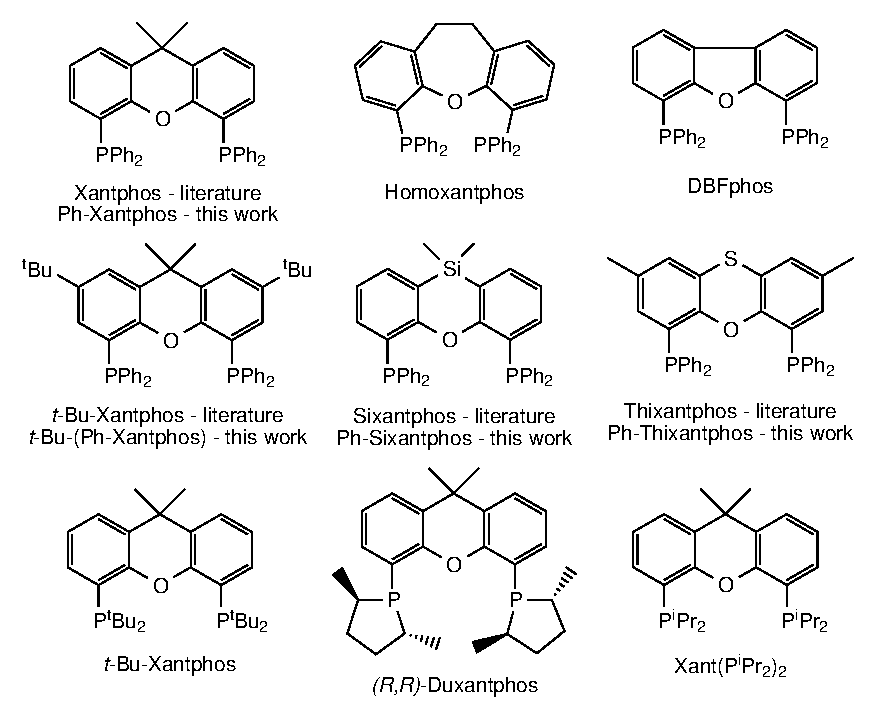
\includegraphics{../Figures/Xantphosligands.eps}
\caption[Examples of the xantphos class of ligands]{Examples of the xantphos class of ligands showing naming and different sites for derivatisation.}
\vspace{0.2cm}
\label{Xantphosligands}
\end{center}
\end{figure}
\vspace{0.2cm}

%A vast number of wide bite-angle ligands based on a xanthene backbone have been synthesised since they were first reported in 1995.\cite{Kranenburg1995, Kamer2001, Esteruelas2011}  The bis-(diphenylphosphino)xanthene ligands were the first wide bite-angle ligands to be systematically studied.  Slight variations in the backbone led to changes in the calculated natural bite-angle.  The derivatives showed significant variations in activity in the rhodium catalysed hydroformylation reacti.  They have since been studied extensively in a range of different reactions \fixme{cite a review or something here} and a number of derivatives have been reported.  

Derivatives of xantphos have focussed mainly on two sites; the bridging group to access a wider range of bite-angles and the phosphine groups.  The phenyl phosphines have been switched for an array for different phosphines including cyclic groups\cite{Veen2000b}, chiral derivatives{\cite{Kamer2001} or changes for solubility.\cite{Buhling1997}  The phosphines have also been switched for different donors including phosphonites,\cite{Dieleman2001} amines, imines, arsines,\cite{Veen2000b} thioethers and others.  Further derivatives with substitutions on the aromatic backbone have also been reported, such as \emph{t}-Bu-(\Phxantphos), or sulfoxantphos,\cite{Goedheijt1998} but are generally less common as changes here have a limited impact due to their distance from the metal.  

Recently an analogue of xantphos has been reported with sterically bulky \tBu{} groups on the phosphines (\tBuXantphos, Figure \ref{Xantphosligands}). First reported in 2005 as a ligand for the palladium catalysed cross-coupling of thiols and aryl bromides or triflates\cite{Mispelaere2005}.  \tBuXantphos{} has since been tested for activity in platinum-catalyzed amination of allylic alcohols\cite{Ohshima2009} and the iron catalysed sp$^3$-sp$^3$ cross-coupling reactions of alkyl halides and alkyl Grignard reagents.\cite{Dongol2007}  However, in each of these cases the complexes were presumed to be formed in the catalytic mixture and were not characterised.  

To date, the only characterised transition metal complexes of \tBuxantphos{} are the series of gold halide complexes [(\tBuxantphos)\ce{Au][AuX2]} where X = Cl$^-$, Br$^-$ or I$^-$.\cite{Partyka2010}  In these structures the \tBuxantphos{} complexes were shown to have large bite angles of 143.0, 142.5 and 143.0\degrees{} for Cl$^-$, Br$^-$ and I$^-$ respectively.  When the same reaction was attempted with the \Phxantphos{} ligands, complexes of the type \ce{[(Xantphos)(AuX)2]} were formed.\cite{Pintado2004, Partyka2010}  These structures clearly indicate the difference between the phenyl and \tBu{} substituted xantphos ligands and the significant impact of the increased steric bulk of the \tBu{} groups on the bonding mode of the ligands.  

The xantphos ligands are widely used in catalysis but \tBuxantphos{} has shown little activity.  This is an indication that the chemistry of the two complexes is substantially different as shown by the only characterised complexes of \tBuxantphos{} reported.  Due to this difference in behaviour further explorations into the coordination activity of \tBuxantphos{} and the reasons for this difference was deemed to be of scientific interest.  Furthermore, the difference in the activity of complexes with \Phxantphos{}, \Phsixantphos{} and \Phthixantphos{} has been previously reported.  Although complexes of \tBuxantphos{} has shown little activity catalytic activity, altering the bridging group, and thus the bite-angle can have a significant impact on the coordination behaviour and the catalytic activity of the complexes produced.  This chapter reports the synthesis of \tBusixantphos{}, \tButhixantphos{} and \tBuxantphos{} along with some of the non-transition metal reactivity of the diphosphines.  

%As these gold complexes are the only examples of characterised tBu-xantphos metal complexes and the phenyl xantphos ligands are so widely utilised the tBu-xantphos ligand system was chosen for further study.  

\section{Ligand Synthesis}\label{section:ligandsynthesis}

In 2002 van Leeuwen \emph{et al.} reported their unsuccessful attempts to synthese \tBuxantphos{} from either the dilithiated backbone or starting with 9,9-dimethyl-4,5-bis(dichlorophosphino)xanthene, suggesting that steric crowding from having two \tBu{} groups on a single phosphorus prevented the successful coupling.\cite{Zuideveld2002}  However, in 2005 a synthesis of \tBuxantphos{} from the dilithiated backbone was reported.\cite{Mispelaere2005}  This synthesis involves lithiation of the backbone using \emph{n}-butyllithium and \gls{TMEDA} in heptane followed by addition of chlorodi-\emph{t}-butylphosphine at 60 \degC{} for 24 hours, generating the product in 38\% isolated yield (Scheme \ref{scheme:Otherligandsynthesis}).

\begin{scheme}[ht]
\begin{center}
\vspace{0.5cm}
\includegraphics{../Schemes/Otherligandsynthesis.eps}
\caption[Literature synthesis of \tBuxantphos]{Literature synthesis of \tBuxantphos{} in heptane.  \emph{i}: \emph{n}-BuLi, \gls{TMEDA}, 15 h. \emph{ii}: \ce{ClP^{t}Bu2}, 60 \degC, 24h.}
\vspace{0.2cm}
\label{scheme:Otherligandsynthesis}
\end{center}
\end{scheme}
\vspace{0.2cm}

%The previously reported synthesis for tBu-xantphos\cite{Mispelaere2005} involved lithiation of the backbone in heptane followed by the addition of chlorodi-\emph{tert}-butyl phosphine and heating to 60\degrees C for 24 hours.  The reportedly air-stable product was obtained and recrystallised from n-propanol in 38\% yield.  Attempts to use this method for the synthesis of tBu-thixantphos yielded a mixture of products.\fixme{check this}

Attempts to utilise the literature method for the synthesis of \tBuxantphos{}\cite{Mispelaere2005} to synthesise \tButhixantphos{} resulted in a number of products which were unable to be identified.  An alternative method using a potassium \emph{tert}-butoxide and \emph{n}-butyllithium ``superbase'' formed a mixture of products from which separation attempts were unsuccessful.  This superbase mixture forms significant amounts of organopotassium compounds, which are more active metallating agents than their organolithium counterparts.  However, organopotassium compounds are also more active in cleavage of ethers.\cite{Bhatt1983}  Hence the mixture of products, may result from cleavage of the ether or thioether bridges resulting in undesired compounds.

%This reference doesn't actually cover organopotassium, just sodium and lithium.

The synthesis of \tButhixantphos{} and \tBusixantphos{} were successfully achieved using the initially reported synthesis of \Phxantphos{}\cite{Kranenburg1995} (Scheme \ref{Ligandsynthesis}).  This method involves the dilithiation of the backbone using \emph{sec}-butyllithium and \gls{TMEDA} followed by reaction with chlorodi-\emph{tert}-butyl phosphine.  Unlike the \Phxantphos{} synthesis which is complete in 16 hours, the synthesis of the \tBu{} ligands required extended periods.  The reaction was allowed to proceed until no further change was determined by NMR (typically 7 days).  NMR analysis of the crude reaction mixture showed the presence of both the mono and diphosphine.  The diphosphine was isolated as white crystals by recrystallisation from \emph{n}-propanol.  The remaining \emph{n}-propanol solution of the monophosphine could be reduced to dryness and then reused for a second lithiation and reaction with chlorodi-\emph{tert}-butyl phosphine to produce more of the desired diphosphine.  

 %carried out in diethyl ether with \gls{TMEDA} using \emph{sec}-butyllithium, added at -78\degrees C followed by addition of the chlorodi-\emph{tert}-butyl phosphine and stirring for 16 hours.  After 16 hours of reaction the NMR spectra showed a mixture of mono and di-substituted products.  The reaction was allowed to proceed until no further change was determined by NMR (typically 7 days).  The reaction invariably produced a mixture of mono and diphosphine.  The diphosphine was separated from the monophosphine by-product by recrystallisation from hot n-propanol and cooling at -16\degC.  The diphosphine was obtained in \fixme{yield} as white crystals.  

\begin{scheme}[ht]
\begin{center}
\vspace{0.5cm}
\includegraphics{../Schemes/Ligandsynthesis.eps}
\caption[Ligand synthesis]{Synthesis of \tBuxantphos{} (X = \ce{CMe2}, R = H), \tButhixantphos{} (X = S, R = Me) and \tBusixantphos{} (X = \ce{SiMe2}, R = H).  \emph{i}: \emph{s}-BuLi, \ce{Et2O}. \emph{ii}: \ce{ClPtBu2}}
\vspace{0.2cm}
\label{Ligandsynthesis}
\end{center}
\end{scheme}
\vspace{0.2cm}

The steric bulk of the \tBu{} groups leads to difficulties in the synthesis of the \tBuxantphos{} ligands.  Reaction with one equivalent of chlorodi-\emph{tert}-butyl phosphine to form the monophosphine is clean and rapid, occurring overnight.  However, the steric bulk of the monophosphine results in a much slower second addition, requiring extended reaction times to allow for significant conversion.  When the reaction is allowed to proceed for longer than one week no additional conversion is observed.  This is likely the result of degradation of either the lithiated monophosphine or the \emph{sec}-butyllithium before the second lithiation can occur.  Over extended periods organolithium reagents cleave diethyl ether resulting in alkanes, alkenes and lithium ethoxide (Scheme \ref{Organolithium}).\cite{Bhatt1983, Gilman1954}  \emph{sec}-butyllithium has been shown to completely react with diethyl ether in one day.\cite{Gilman1954}  Although the reaction between diethyl ether and phenyllithium is slower (half-time of 100 hours), the extended reaction periods required for the second phosphine addition mean that this degradation pathway may limit the reactivity.  \fixme{cite Schlosser organometallics in organic synthesis}

%Between \emph{n}-butyllithium the reaction occurs with a half time of 6 days at 25\degC{}.\fixme{ref}  Although an aryl lithium with an ortho oxygen group would be expected to reaction more slowly with the diethyl ether this is one possible pathway for reaction.  \fixme{does this happen in THF}  

%This is likely a result of the steric bulk of the \emph{tert}-butyl groups hindering the second addition reaction.  However, over time organolithium reagents react with diethyl ether generating lithium ethoxide and ethene (Scheme \ref{Organolithium}).  This reaction occurs with a half time of 6 days at 25\degC{} for \emph{n}-butyllithium.  This is likely the reason for the lack of observed reaction after periods of one week.

\begin{scheme}[ht]
\begin{center}
\vspace{0.5cm}
\includegraphics{../Schemes/Organolithium.eps}
\caption[Reaction of n-butyllithium with diethyl ether]{Reaction of n-butyllithium with diethyl ether}
\vspace{0.2cm}
\label{Organolithium}
\end{center}
\end{scheme}
\vspace{0.2cm}

In order to promote the dilithiation, a preformed sec-butyllithium, \gls{TMEDA} complex was added to a solution of the backbone.  An initial colour change to yellow (\tButhixantphos{} and \tBusixantphos) or green (\tBuxantphos) was observed, indicative of monolithiation.  After stirring overnight this changed to red or yellow respectively.  This colour change gives a clear indication of successful dilithiation.  In order to favour the diphosphine over the monophosphine the lithiated backbone was then added slowly to an ethereal solution of chloro-di-\emph{t}-butylphosphine.  Although a mixture of the mono- and diphosphine was always obtained this order of addition was found to be more successful, resulting in increased yields.

The \tBuxantphos{} ligand obtained using our method had \proton{} and \carbon{} NMR spectra consistent with the literature.\cite{Mispelaere2005} However the \phosphorus{} chemical shift differed by 2.2~ppm (10.2~ppm in this study compared to 12.4 ppm).  The NMR spectra for the reported and the synthesised samples were both obtained in \ce{CDCl3} and referenced to an external 85\% \ce{H3PO4} standard.  Hence the reason for this difference is unclear.  However, as the remainder of the NMR and other characterisation data is consistent, it is likely that the two compounds are identical and a typographical error or otherwise was made in the preparation of the earlier paper.

The synthesis of these ligands utilises directed ortho metallation as first described independently by Gilman and Wittig in 1939 and 1940 respectively.\cite{Gilman1939, Wittig1940} Directed \emph{ortho} metallation uses a heteroatom which can coordinate to the organolithium thereby directing it to the \emph{ortho} sites.  In this case the ether linkage can act as a director for the lithiation.  Once lithiated the electron density on the oxygen stabilises the lithiated site against degradation.  For \tBuxantphos{} and \tBusixantphos{} the oxygen is the only atom present with lone pairs of electrons and thus the lithiation occurs exclusively in the desired positions \emph{ortho} to the oxygen.  However, phenoxathiin has both an ether and a thioether which can both act as \emph{ortho}-directors.\cite{Organolithiummethods}  Previous research shows that in the presence of both ether and thioether groups the lithiation will occur \emph{ortho} to the oxygen.\cite{Turck1997}  However, once the first lithiation has taken place the oxygen is unable to contribute significantly to the second lithiation.  For \tBuxantphos{} and \tBusixantphos{} the influence of the oxygen is still sufficient that the second lithiation occurs in the other ortho position.  However for phenoxathiin the thioether acts as a second directing group and the lithiation occurs \emph{ortho} to the sulfur (Scheme \ref{scheme:transthixantphos}).  The addition of methyl groups in the postion \emph{meta} to the thioether, prevents the sulfur from acting as a director, resulting in the desired \tButhixantphos{} ligand.  

%The methyl groups on the aromatic system of \tButhixantphos{} was found to be important.  The attempted synthesis of a \tButhixantphos{} without methyl groups resulted in substitution ortho to the oxygen and ortho to the sulfur in a transoid configuration (Scheme \ref{Transthixantphos}).  It is likely that using three equivalents of \emph{sec}-butyllithium results in lithiation in three positions, the two ortho to the oxygen and one ortho to the sulfur.  The first addition of phosphine attacks one ortho to the oxygen.  This creates increased steric hindrance at the second site ortho to oxygen so the second equivalent of phosphine preferentially attacks in the least hindered site; ortho to the sulfur.  \fixme{this paragraph may in fact just be lies}.  The oxygen in the bridge of all three ligands acts as a directing group to promote lithiation in the ortho position.  However in the case of \tButhixantphos{} the sulfur can also act as a directing group (though less strongly that the oxygen) this leads to competition for the lithiation site and requires the methyl on the backbone to provide steric hindrance and prevent lithiation ortho to the sulfur.  This difficulty was not encountered with either the \tBuxantphos{} or \tBusixantphos{} ligands.  The carbon and silicon groups are not able to interact with the lithium and promote ortho lithiation so the lithiation occurs exclusively ortho to the oxygen. \fixme{see directed ortho lithiation for more info}

\begin{scheme}[ht]
\begin{center}
\vspace{0.5cm}
\includegraphics{../Schemes/Transthixantphos2.eps}
\caption[Influence of methyl groups on the synthesis of \tButhixantphos]{Influence of methyl groups on the synthesis of \tButhixantphos. \emph{i}: \emph{sec}-BuLi, \ce{Et2O}. \emph{ii}: \ce{ClPtBu2}}
\vspace{0.2cm}
\label{scheme:transthixantphos}
\end{center}
\end{scheme}
\vspace{0.2cm}

%However, the synthesis of \tBusixantphos{} was not problem free.  Given the extended reaction times necessary to obtain the diphosphines, the formed diphosphine is in solution with large volumes of lithium chloride for a substantial amount of time.  NMR analysis of the synthesis of \tBusixantphos{} showed the formation of a significant amount of a compound with a single peak in the \phosphorus{} NMR spectrum at 15 ppm.  No new peaks were observed in the \proton{} NMR spectrum.  However, due to the similarity in the spectra to those of \tBusixantphos H+ we propose that this compound is [Li\tBusixantphos]Cl.  The compound is unchanged through extensive water washing.  Attempts to remove the lithium ion using the lithium specific chelating agent, 12-crown-4, were unsuccessful.  Reaction with tetrafluoroboric acid in order to exchange the lithium for a proton led to the formation of a new species the nature of which could not be determined.  The formation of [Li\tBusixantphos]Cl results in a significant loss of product for the synthesis of \tBusixantphos{} resulting in lower yields than those for \tBuxantphos{} and \tButhixantphos{}.

%It was found the \tBusixantphos{} tended to capture lithium ions between the two phosphorus atoms.  These lithium ions were tightly bound and were retained through several cycles of washing with water.  The nature of this species was confirmed by reaction with a sample of the pure ligand with lithium chloride, resulting in the same product.  \fixme{do this} Attempts to react the lithiated \tBusixantphos{} with tetrafluoroboric acid to exchange the lithium ion for a proton was unsuccessful and instead resulted in possibly a boron trifluoride bound between the two phosphines.\fixme{check this with boron NMR etc.}  Attempts to remove the lithium using the lithium specific chelating agent, 12-crown-4, were unsuccessful.  Due to the inability to remove the lithium this represents a source of significant loss of product for the synthesis of \tBusixantphos{} resulting in lower yields than those for \tBuxantphos{} and \tButhixantphos{}.

The NMR data of the newly reported \tButhixantphos{} and \tBusixantphos{} ligands are consistent with expectations (Table \ref{table:ligandNMRdata}).  In both cases a plane of symmetry reduces the number of signals hence showing a single peak in the \phosphorus{} NMR.  The \phosphorus{} chemical shift for \tBuxantphos{} synthesised in this work is 10.2 which differs from the reported value of 12.4\cite{Mispelaere2005}, however the \proton{} and \carbon{} data is consistent.  The \phosphorus{} chemical shifts for the \tBusixantphos{} and \tButhixantphos{} ligands are observed as singlets at 8.4 and 9.5 respectively.  The \proton{} NMR for the aromatic system is as expected, with two singlets present for \tButhixantphos, and a doublet, doublet of doublets and a triplet observed for \tBusixantphos{} and \tBuxantphos.  The chemical shift of the methyl substituents differs for each ligand, as expected.  In \tBusixantphos{} the dimethylsilyl group appears at 0.46 ppm, close to the tetramethylsilane reference.  In \tBuxantphos{} the bridgehead methyls appear at 1.57 ppm, within the typical range for organic methyl groups.  The methyl groups in \tButhixantphos{} are evident at 2.25 ppm, consistent with methyl substituents attached to aryl rings.  

\begin{table}[ht]
\small
\caption[Selected NMR Data for Xantphos Ligands]{Selected NMR Data for Xantphos Ligands in \ce{CDCl3}}
\vspace{1em}
\label{table:ligandNMRdata}
\begin{center}
\begin{tabular}{l c c c c c c}
	\toprule
	~\bfseries{Diphosphine} & \bfseries{$\delta$P (ppm)} & \multicolumn{5}{c}{\bfseries{$\delta$H (ppm)}} \\
	\midrule		
	~\tBuXantphos\cite{Mispelaere2005}	& 12.4 & 1.21-1.26 & 1.57 s & 7.02 t & 7.38 dd & 7.60 d\\
	~\tBuXantphos{}(This work) 		& 10.2 & 1.21-1.25 & 1.57 s & 7.03 t & 7.38 dd & 7.60 d\\
	~\tBuThixantphos				& 9.5 & 1.22-1.24 & 2.25 s & 6.88 s & 7.29 s & \\
	~\tBuSixantphos				& 8.4 & 1.29 vt & 0.46 s & 7.12 t & 7.53 d & 7.87 d\\ 
	\bottomrule{}
\end{tabular}
\end{center}
\end{table}

The \proton{} NMR data for the \tBuxantphos{} ligands show a complex \ce{X18A}A'\ce{X18}' spin system for the \tBu{} protons.  For a system where the two A atoms (in this case the phosphorus atoms) are strongly coupled this leads to interaction between the three and five bond couplings (e.g. when the phosphorus atoms are in a trans configuration in a metal complex) resulting in a virtual triplet.  However, in this case there is no atom between the phosphorus atoms so we would expect a three-bond and a nine-bond coupling.  A nine-bond coupling is an extremely remote coupling which we would expect to be negligible.  Based on previous reports\cite{Harris1964, Abraham1961} this peak shape with two sharp outer lines and a broad inner peak occurs when the difference between the short and long range couplings is very small but not zero.  For this to occur the phosphines must have some degree of through-space spin-spin coupling through their lone pairs of electrons (for a review of nonbonded spin-spin coupling see Hierso\cite{Hierso2014}).  This is further supported by the difference in the \proton{} spectra for the three ligands; the central peak is sharpest for \tBusixantphos{} then \tButhixantphos{}.  For \tBuxantphos{} some further detail can be seen indicating that this has the weakest through space coupling.  This trend is consistent with the expected changes in the distance between the phosphines upon changing the backbone which will impact the degree of through-space coupling that can occur and therefore the difference in the short and long-range coupling constants.

%include spectra showing the tBu peak?

\section{Bite Angle Calculations}

The steric and electronic properties of diphosphine ligands determines their complexation behaviour with transition metals and can influence the reactivity of the complex, particularly impacting the activity and selectivity in catalytic transformations.\cite{Freixa2003, Birkholz2009}  The xantphos class of ligands were initially investigated as ligands with consistent electronic properties and steric bulk so that the impact of the bite-angle on rhodium catalysed hydroformylation could be studied exclusively.\cite{Kranenburg1995}  Consequently a number of studies have investigated the bite-angle impact on a variety of catalytic conversions (for examples see\cite{Kranenburg1995b, Haaren2001b, Dudle2011b, Fanjul2013, Birkholz2009}).  However, it has since been determined that the bite-angle is a result of both the steric and electronic properties of the ligand.\cite{Freixa2003}

The natural bite-angle (\natbiteangle) was first described by Casey and Whiteker\cite{Casey1990} as a theoretically determined parameter to indicate the preferred chelation angle of diphosphine ligands irrespective of the metal they are coordinating to.  Computationally these are calculated using a rhodium atom at 2.3 \si{\angstrom} and optimising the geometry of the ligand system, the natural bite-angle can then be measured.  This is often used in combination with a flexibility range (the bite-angles that can be obtained within a range of 12.6~\si{\kilo\joule\per\mol}).  

Despite the ubiquity of the natural bite-angle within diphosphine chemistry no studies have investigated whether the natural bite-angle has proven to be an apt predictor of the crystallographically determined bite-angle.  In order to determine the usefulness of the natural bite-angle in determining the coordination bite-angle an investigation into this, using data from the \gls{CSD} was performed.  The results are summarised in Table \ref{table:biteangles} and Figure \ref{Biteanglegraph}.  The natural and median experimental bite-angles show a good correlation described by the equation $\Theta$\sub{exp} $= 1.1013$\natbiteangle $- 5.6972$, ($R^2 = 0.9246$).  Some of the experimental and natural bite-angles that are most relevant to this work show significant differences (for example \tBuxantphos{} \natbiteangle{} = 140\degrees, experimental = 153.317\degrees and \Phsixantphos{} \natbiteangle{} = 109, experimental = 99.165\degrees) this may be due to the low numbers of structures for these ligands (4 and 5 respectively) at which point the metals used will have a significant impact. 

\begin{table}[htb]
\small
\caption[Crystallographic bite-angles for diphosphine ligands]{Crystallographic bite-angles for diphosphine ligands, taken from the Cambridge Crystallographic Data Centre.} 
\vspace{1em}
\label{table:biteangles}
\begin{center}
\begin{tabular}{c c c c c c}
	\toprule
	~~\bfseries{Diphosphine}~~ & \bfseries{Structures} & \bfseries{P-P ($\si{\angstrom}$)} & \bfseries{Range (\degrees)} & \bfseries{Bite-Angle (\degrees)} & \bfseries{$\beta$\sub{n} (\degrees)}\\
	\midrule
	 ~dppm			& 384	& 2.718	& 62.757 - 77.706 	& 71.062 	& 73	\\
	 ~dppe			& 1939	& 3.095	& 71.073 - 92.926	& 83.818	& 78 \\
	 ~dppp			& 3237	& 3.308	& 83.333 - 105.420	& 92.181	& 86 \\ 
	~BINAP			& 146	& 3.296	& 85.9820 - 115.666	& 91.925	& 92 \\
	~dppb			& 127	& 3.391	& 89.447 - 111.491	& 94.240	& 99 \\
	 ~DPEphos		& 101	& 3.844	& 96.094 - 158.531	& 112.691	& 102 \\
	 ~\PhXantphos		& 65		& 3.908	& 98.829 - 153.134	& 108.535	& 111 \\
	 ~BISBI			& 4		& 4.079	& 103.533 - 151.951	& 124.789 & 123 \\
	~Ph-sixantphos		& 5		& 3.691 	& 95.250 - 152.149	& 99.165 & 109 \\
	~Ph-thixantphos	& 3		& 4.021	& 109.528 - 155.050	& 111.724	& 110 \\
	~tBu-xantphos		& 4		& 4.527	& 152.302 - 153.456 & 153.317 & 140 \\
	~dpp-benzene		& 116	& 3.101	& 74.380 - 92.499	& 84.900	& 83\\
	~dppn			& 25		& 3.176	& 79.867 - 93.270	& 86.864	& 82 \\
	~dppx			& 19		& 3.569	& 90.045 - 106.186	& 102.636	& 90 \\
	~dbpe			& 109	& 3.200	& 83.989 - 95.949	& 90.369	& 87	\\
	~dbpp			& 12		& 3.503	& 94.556 - 104.857	& 99.175	& 99	\\
	~dbpx			& 10		& 3.634	& 98.758 - 107.255	& 101.881	& 101 \\
	\bottomrule{}
\end{tabular}
\end{center}
\end{table}

\begin{figure}[htb]
\begin{center}
\vspace{0.5cm}
\includegraphics[width=\textwidth]{../Figures/Biteanglegraphorigin.eps}
\caption[Comparison of the Natural Bite-Angle with the Experimentally Determined Bite-Angle]{Comparison of the Natural Bite-Angle with the Experimentally Determined Bite-Angle.  Trendline $ y = 1.1013x - 5.6972$, Linear regression $R^2 = 0.9246$}
\vspace{0.2cm}
\label{Biteanglegraph}
\end{center}
\end{figure}
\vspace{0.2cm}

In order to determine the potential differences between the \tBu{} and Ph xantphos ligands, the natural bite-angles of the three \tBuxantphos{} ligands were calculated.  Bite-angle calculations are typically carried out using molecular mechanics, in this study we used a \gls{DFT} instead, hence the natural bite-angles of the previously reported \Phxantphos{} series of ligands and \tBuxantphos{} (Table \ref{table:biteanglescalculated}).  The structures were optimised using the B3LYP functional\cite{Becke1993, Lee1988, Vosko1980, Stephens1994} with the def2-TZVP basis set.\cite{Andrae1990, Weigend2005} using a Rh-P distance of 2.315 \si{\angstrom}.  The values calculated using \gls{DFT} are typically larger than those reported using molecular mechanics (Table \ref{table:biteanglescalculated}).\fixme{why?}

%These show good agreement with those calculated using molecular mechanics.  Given the good agreement of our DFT obtained values and the literature values we continued by calculating the bite-angles for the two new ligands \tButhixantphos{} and \tBusixantphos{}.  A number of different bite-angles have been reported for the \Phxantphos{} series, due to different computational set-ups.  

\begin{table}[ht]
\small
\caption[Bite angles of xantphos ligands]{Bite angles of xantphos ligands}
\vspace{1em}
\label{table:biteanglescalculated}
\begin{center}
\begin{tabular}{c c c c}
	\toprule
	~\bfseries{Diphosphine}	&\bfseries{Molecular Mechanics (\degrees)}&\bfseries{Reference}	&\bfseries{DFT (\degrees)}\\
	\midrule		
	~\PhXantphos		~~&~108, 111.7~~	& ~\cite{Birkholz2009}	&~~118.59~~	\\	
	~\PhThixantphos	~~&~110, 109.4~~	& ~\cite{Birkholz2009, Kranenburg1995}&~~118.04~~	\\
	~\PhSixantphos	~~&~108, 108.7~~	& ~\cite{Birkholz2009, Kranenburg1995}&~~111.43~~	\\
	~\tBuXantphos		~~&~140~~		&~\cite{Birkholz2009}~~	&~~159.93~~	\\
	~\tBuThixantphos	~~&~~~			&~~~~			&~~126.98~~	\\
	~\tBuSixantphos	~~&~~~			&~~~~			&~~126.80~~	\\
	\bottomrule{}
\end{tabular}
\end{center}
\end{table}

%  including allylic alkylations\cite{Haaren1999}, rhenium catalysed hydrogenation\cite{Dudle2011b} and the palladium catalysed hydromethoxycarbonylation of ethene.\cite{Fanjul2013}  
%reviews have investigated whether the bite-angle impact is 

The natural bite-angles for the \tBuxantphos{} series of ligands are much larger than for the phenyl substituted ligands.  Given that the remainder of the ligands is unchanged, this effect is due to the impact of the \tBu{} groups.  These groups are more electron donating than the phenyls so may result in more electron density on the phosphorus atoms resulting in an electrostatic repulsion of the two phosphorus atoms.  The \tBu{} groups have a larger steric impact than the planar phenyl rings.  This would result in a larger bite-angle as the steric bulk of the \tBu{} substituents pushes the two phosphorus atoms further apart.  The trend between the two groups is the same with the carbon bridged having the largest \biteangle{} and the silicon bridged having the smallest.

The bite-angles of the \tBuxantphos{} ligands is likely to have a significant impact on their coordination chemistry.  The phenyl ligands form a range of complexes favouring \cis-chelation in square-planar and octahedral complexes, although \emph{trans} square planar complexes have been reported\cite{Petocz2004}.  With bite-angles of 126.8-159.9\degrees{} the ligands will likely prefer trigonal planar coordination environments close to 120\degrees.  However the bite-angles are halfway between the \cis{} and \trans{} coordination angles for square planar complexes which may result in mixtures of products.  The ratio between the two geometries may change depending on which ligand is used with \tBusixantphos{} favouring \cis-coordination while \tBuxantphos{} favours the \trans-coodination.  However, the steric demands of the \tBu{} substituents may promote the \trans{} chelation.  

Diphosphine ligands that exhibit exclusive \trans-chelation have been described in a review as elusive.\cite{Freixa2008}  \PhXantphos{} itself can form \trans-chelates\cite{Petocz2004}, however these form as a mixture of the \cis and \trans isomers rather than forming as the pure \trans isomer.  Only a small number of these \trans-chelates for \Phxantphos{} have been reported compared to the majority of complexes where the \cis-chelate forms.  A limited number of ligands exist that can form \trans-chelates, however, rarer are those that do not form \cis-chelates and rarer still are the truly \trans-chelating ligands with a bite-angle of 180\degrees{} and an undistorted coordination plane. 

The wide bite-angles of these ligands may also result in interesting catalytic activity.  Previously reported uses of \tBuxantphos{} have added the ligand to a metal precusor and formed the catalyst in situ.  However platinum(II), palladium(II) and iron prefer either square-planar or octahedral coordination and if the \tBuxantphos{} ligand coordinated in a \trans{} configuration this may prevent the reductive elimination of other ligands.  Hence although \tBuxantphos{} has not shown activity in catalytic systems to date, these ligands may find more use in systems with metals able to form tetrahedral, trigonal planar, or pyramidal structures such as silver or rhodium, or platinum and palladium(0).

%\section{Oxidation}

%Although previous literature reports \tBuxantphos\cite{Mispelaere2005} as an air-stable solid, this was not the case for at least \tButhixantphos.  The ligands are resistant to oxidation and can be handled in the air for short periods.  However, storage in the air leads to slow oxidation.  

%The ligands appear to be more stable to oxidation using hydrogen peroxide than \Phxantphos{}.  Although the \tBuxantphos{} ligands oxidise slowly in the air which \Phxantphos{} does not; attempts to directly oxidise using a large excess of hydrogen peroxide in acetone requires extended periods of reflux while \Phxantphos{} undergoes complete oxidation after only 1 hour at room temperature.\cite{Jahromi2012}

%However problems were encountered with this as the thioether bridge is also susceptible to oxidation.  As such attempts to oxidise the phosphines of \tButhixantphos resulted in oxidation of one of the phosphine arms and the thioether bridge to a sulfoxide or sulfone resulting in a mixture of products.  

\section{Basicity}
\label{section:ligands:basicity}

During the synthesis of the \tBuxantphos{} ligands, particularly for \tBusixantphos{} a small amount of a by-product was observed by \phosphorus{} and \proton{} NMR spectroscopy.  The \proton{} NMR spectra suggested the presence of an additional proton environment.  Leaving the ligands for extended periods in \ce{CDCl3} resulting in increased amounts of this impurity over time, suggesting that the formed \tBuxantphos{} ligands were undergoing reaction with the solvent rather than the impurity forming in the synthesis of the ligands.  Over time chloroform is known to undergo degradation forming hydrochloric acid.\cite{Yano1977}  Furthermore tertiary phosphines are known to act as Br\o nsted bases, forming phosphonium ions that can be used as components in catalytic reactions.\cite{Netherton2001}  Hence, the identity of these compounds as phosphonium salts seemed likely.

%As discovered during the synthesis of \tBusixantphos{} the ligands have the ability to coordinate small cations.  Although only \tBusixantphos{} coordinated lithium to any significant degree during the synthesis, all three of the ligands are significantly acid sensitive and will react with any adventitious proton source resulting in the protonation at one of the phosphines.  Although stable for short periods in deutero-chloroform, over time chloroform produces hydrochloric acid \emph{via} photo-degradation which readily protonates the ligands

Reaction of the \tBuxantphos{} ligands with either of the strong acids \ce{CHPh(SO2CF3)2} (\pKa = 2.0 in DMSO) or \ce{CH2(SO2CF3)2} (\pKa = 2.4 in DMSO), results in immediate formation of a phosphonium salt (Scheme \ref{Protonation}).  These acids are useful as they are non-hygroscopic solids allowing for accurate stoichiometry.  However, addition of excess acid results in the same product, no evidence for an additional protonation was observed.  The NMR data is consistent with the data for the impurity observed in the synthesis of the \tBuxantphos{} ligands, indicating that the impurity is [\tBuxantphos(H)\ce{]+}.

\begin{scheme}[ht]
\begin{center}
\vspace{0.5cm}
\includegraphics{../Schemes/Protonation.eps}
\caption[Protonation of the ligands using a strong acid]{Protonation of the ligands using a strong acid}
\label{Protonation}
\end{center}
\end{scheme}
\vspace{0.2cm}

Selected NMR data for the phosphonium salts [\tBuxantphos\ce{(H)]+} is given in Table \ref{table:protonatedNMR}.  A broad singlet is present in the \phosphorus{} NMR spectra for the three phosphonium ions shifted slightly downfield of the free ligand.  Similarly half the expected number of peaks is observed in the \proton{} and \carbon{} NMR spectra.  This indicates that although the complex is mono-cationic the system is undergoing a dynamic process such that the two halves of the molecule are equivalent on the NMR timescale.  The most likely process is the exchange of the proton between the two phosphorus atoms.  The \proton{} NMR spectra all show a complex spin system of the type XAA\textprime X for the phosphonium proton, which is further evidence for the dynamic exchange of the proton between the two phosphorus atoms.  

\begin{table}[htbp]
\caption[Selected NMR data for [\tBuxantphos(H){]}\ce{CH(SO2CF3)2}]{Selected NMR data for the [\tBuxantphos(H){]}\ce{CH(SO2CF3)2} compounds}
\label{table:protonatedNMR}
\small
\begin{center}
\begin{tabular}{l c c c}
	\toprule{}
	~~ & \multicolumn{2}{c}{\bfseries{\phosphorus}} & \bfseries{\proton}\\
	\cmidrule(lr){2-3} \cmidrule(lr){4-4}
	\bfseries{Ligand}&\bfseries{$\delta/$ppm}&\bfseries{$\Delta\delta/$ppm}& \bfseries{\ce{H+}$\delta/$ppm}\\
	\midrule{}
	\tBuSixantphos		& 14.3	& 5.9 	& 9.57 \\
	\tBuThixantphos 	& 15.8	& 6.3		& 8.99 \\
	\tBuXantphos		& 17.4	& 7.2		& 8.57 \\
	\bottomrule{}
\end{tabular}
\end{center}
\end{table}

The difference in the rate of exchange of the proton in the three compounds in clearly shown by the \phosphorus{} and \proton{} NMR spectra.  The \phosphorus{} NMR signal is sharpest for \tBusixantphos{} followed by \tButhixantphos{} while \tBuxantphos has a very broad signal.  Indicating the exchange is fastest for \tBusixantphos{} and slowest for \tBuxantphos{}.  The \proton{} NMR spectra (Figure \ref{Protonatedligandsnmr}) show an XAA'X spin system for the phosphonium proton.  The signal appears most like a virtual triplet for \tBusixantphos{} indicating very little different in the coupling constants of the proton with each phosphorus.  For \tButhixantphos{} the central peak has broadened slightly, while in \tBuxantphos{} the central peak is very broad indicating that the difference in the two coupling constants is increasing.  Furthermore the chemical shift of the phosphonium proton is different  for the three systems (\tBusixantphos{} = 9.57, \tButhixantphos{} = 8.99 and \tBuxantphos{} = 8.57~ppm).  This indicates that the \tBusixantphos{} proton is less shielded and thus has a faster rate of exchange while \tBuxantphos{} proton is the most shielded and has the slowest rate of exchange.  This trend is consistent with the bite-angles for the ligands.  \tBusixantphos{} has the smallest bite-angle and thus the two phosphorus atoms are closer resulting in a lower barrier to exchange, whilst \tButhixantphos{} has the largest bite-angle and thus the slowest exchange.  

%The \phosphorus{} NMR spectrum has a single broad signal at 15.8 ppm showing a downfield shift of 6.3 ppm upon protonation.  In the \proton{} NMR spectrum the phosphonium proton comes at 9.0~ppm much higher than other phosphonium ions.  In addition the proton appears as an unusual signal in a 1:2:1 ratio with two sharp outer peaks and a broad inner peak.  The \phosphorus{}, \proton{} and \carbon{} spectra show half of the expected peaks indicating a plane of symmetry through the central bridge of the molecule.  However, the signal for the phosphonium proton only integrates for a single proton.  Together with the broadness of the \phosphorus{} and some of the \carbon{} signals this indicates a dynamic system in solution with proton exchange between the two phosphorus atoms.   \fixme{this data is for the sulfur bridged ligand should I include stuff for silicon as well?} 

\begin{figure}[htb]
\begin{center}
\vspace{0.5cm}
\includegraphics[scale = 0.8, trim = 1.5cm 10cm 4.5cm 5cm, clip]{../NMR/Phosphoniumstacked.eps}
\caption[\proton{} NMR spectra for \tBusixantphos, \tButhixantphos{} and \tBuxantphos{} showing the P-H region]{\proton{} NMR spectra in \ce{CDCl3} at 20\degC{} for \tBusixantphos, \tButhixantphos{} and \tBuxantphos{} (Si, S and C respectively) showing the P-H region}
\vspace{0.2cm}
\label{Protonatedligandsnmr}
\end{center}
\end{figure}
\vspace{0.2cm}


%\begin{figure}[htp]
%\begin{center}
%\vspace{0.5cm}
%\includegraphics[scale=0.85]{../Figures/VTNMR/Protonatedligands.pdf}
%\caption[\proton{} NMR spectra for \tBusixantphos, \tButhixantphos{} and \tBuxantphos{} showing the P-H region]{\proton{} NMR spectra in \ce{CDCl3} at 20\degC{} for \tBusixantphos, \tButhixantphos{} and \tBuxantphos{} (Si, S and C respectively) showing the P-H region}
%\vspace{0.2cm}
%\label{Protonatedligandsnmr}
%\end{center}
%\end{figure}
%\vspace{0.2cm}

The dynamic behaviour of the phosphonium ions was further investigated using variable temperature \phosphorus{} and \proton{} NMR experiments on [(\tButhixantphos)H]\ce{CH(SO2CF3)2} (Figure \ref{VTStBuH})  At room temperature a single peak is present in the \phosphorus{} NMR spectrum.  When heated this peak shifts slightly to higher ppm and becomes sharper.  This single peak indicates that the exchange of the proton between the two phosphorus atoms is occuring rapidly enough that the two phosphorus atoms appear to have the same environment on the NMR timescale.  Cooling below room temperature causes the singlet to broaden significantly with coalescence occurring around -40\degC{}.  At -60\degC{} two signals are present though they are still broad.  One of these signals resolves into a doublet at -80\degC, however the other peak is still very broad ranging from 11-23 ppm.  Given the chemical shift of the free ligand it is likely that the sharp doublet belongs to the unprotonated phosphorus and the broad peak is the protonated phosphorus.  This is also consistent with the shift of the peaks at higher temperature where we observe a shift to higher ppm as the rate of exchange is increased.  

\begin{figure}[h!]
\begin{center}
\vspace{0.5cm}
\includegraphics[scale=0.8, trim = 0cm 6.8cm 0cm 2cm]{../NMR/PhosphoniumVTNMRboth.eps}
\caption[Variable temperature \phosphorus{} and \proton{} NMR data for {[}(\tButhixantphos)H{]}\ce{CH(SO2CF3)2}]{Variable temperature \phosphorus{} (right) and \proton{} (left) NMR data for [(\tButhixantphos)H]\ce{CH(SO2CF3)2}}
\vspace{0.2cm}
\label{VTStBuH}
\end{center}
\end{figure}
\vspace{0.2cm}

%\begin{figure}[h!]
%\begin{center}
%\vspace{0.5cm}
%\includegraphics[scale=0.8]{../Figures/VTNMR/StBuHboth.pdf}
%\caption[Variable temperature \phosphorus{} and \proton{} NMR data for {[}(\tButhixantphos)H{]}\ce{CH(SO2CF3)2}]{Variable temperature \phosphorus{} (right) and \proton{} (left) NMR data for [(\tButhixantphos)H]\ce{CH(SO2CF3)2}}
%\vspace{0.2cm}
%\label{VTStBuH}
%\end{center}
%\end{figure}
%\vspace{0.2cm}

The variable temperature \proton{} NMR data for [\tButhixantphos\ce{H]CH(SO2CF3)2} (Figure \ref{VTStBuH}) shows similar changes as the \phosphorus{} NMR spectra.  At low temperature the proton is static on a single phosphorus atom so we observe a doublet.  As the temperature increase to -20 \degC{} we observe a broad signal appearing in the centre of the doublet as exchange begins to occur and the signal changes from a simple doublet to a XAA'X' spin system.  This signal increases and at 20 \degC{} all three peaks begin to broaden again with coalescence at 50 \degC. This broadening is possibly the result of the proton no longer being isolated on a single molecule but delocalised across the entire system.   

Typically \phosphorus{} NMR spectra are proton decoupled.  However, with very strongly coupled systems such as phosphonium ions the decoupler is not able to fully decouple the spin system resulting in broadening and side bands.  To further investigate the [\tButhixantphos\ce{H]CH(SO2CF3)2} system, proton coupled phosphorus NMR spectra were obtained at room temperature and -80\degC{} (Figure \ref{VTStBuHcoupled}).  At room temperature a simple doublet appears, as expected.  This indicates rapid movement of the proton between the two phosphorus atoms thus coupling with both.  When cooled to -80\degC{} the \phosphorus\{\proton\} spectrum showed a doublet and a broad singlet.  In the proton coupled phosphorus spectrum the doublet is retained confirming that this is the non-protonated phosphorus showing coupling to the protonated phosphorus.  The broad singlet resolves into a doublet of doublets with coupling constants consistent with coupling to the proton and the other phosphorus.  This further confirms that no exchange of the proton is occurring at low temperature.  

\begin{figure}[htp]
\begin{center}
\vspace{0.5cm}
\includegraphics[scale = 0.8, trim = 0cm 8cm 0.5cm 10cm, clip]{../NMR/Coupledstacked.eps}
\caption[Variable temperature proton coupled \phosphorus{} NMR spectra for (\tButhixantphos)H+]{Variable temperature proton coupled \phosphorus{} NMR data for (\tButhixantphos)H+}
\vspace{0.2cm}
\label{VTStBuHcoupled}
\end{center}
\end{figure}  
\vspace{0.2cm}


%\begin{figure}[htp]
%\begin{center}
%\vspace{0.5cm}
%\includegraphics[scale=0.8]{../Figures/VTNMR/StBuHcoupled.pdf}
%\caption[Variable temperature proton coupled \phosphorus{} NMR spectra for (\tButhixantphos)H+]{Variable temperature proton coupled \phosphorus{} NMR data for (\tButhixantphos)H+}
%\vspace{0.2cm}
%\label{VTStBuHcoupled}
%\end{center}
%\end{figure}  
%\vspace{0.2cm}

%The protonation of the ligands was carried out using either or .  These are both strong acids with \pKa s of 2.0 and 2.4 in DMSO.\cite{Koppel2000}  The direct protonation of the ligands using a strong acid resulted in the phosphonium ions shown in Scheme \ref{Protonation}. 

%The degree of dynamism changes between the three ligands.  The sulfur bridged ligand with the smallest \biteangle{} has the greatest degree of exchange between the systems \fixme{can I get temperatures for coalescence as this would prove it nicely}.  \fixme{the S has the middle one need to check how much coupling in the carbon one}  The sulfur bridged ligand has very little coupling evident in the NMR spectra compared to the silicon bridged ligand which has a number of clearly defined coupled peaks.  The silicon bridged ligand has the largest degree of exchange at room temperature as the phosphorus atoms are held much closer - as shown by the smaller \biteangle{} which would indicate a greater degree of interaction between the tertiary phosphine and the phosphonium ion and thus much more rapid exchange.  As such at room temperature we are below coalescence and thus the NMR peaks resolve into much clearer signals than those found with the sulfur or carbon bridged systems.

%Likewise the carbon bridged system with the largest \biteangle{} will have the smallest degree of exchange at room temperature.  Hence we are closer to coalescence than in the other two so the NMR spectra are very broad and unable to be fully assigned.  \fixme{check the NMR data for 3013 on 600 MHz}

%Variable temperature phosphorus and proton NMR data for is shown in Figures \ref{VTStBuHphosphorus} and \ref{VTStBuHproton}

Colourless crystals of [\tButhixantphos(H)]\ce{CPh(SO2CF3)2} suitable for X-ray diffraction were grown from the reaction mixture in benzene.  The compound crystallised with a benzene solvate, as 2\ce{[StBu-xantphos(H)]CPh(SO2CF3)2}$\cdot{}$\ce{C6D6} in the monoclinic space group \emph{P}2\sub{1}/\emph{n}.  Selected bond lengths and angles are summarised in Table \ref{table:crystalprotonated:lengths} and crystallographic data is given in Table \ref{table:crystalprotonated:data}.  Although the cationic portion was well refined one of the counterions is disordered with two positions for the \ce{SO2CF3} chains.  The proton on the phosphonium ion was able to be found and is exclusively located on a single phosphorus atom.  As a result of this the \gls{esd} on the bond lengths and angles involving this proton are relatively high.  The distances from the proton to the other phosphorus or to the oxygen atom are both too long to indicate any degree of interaction.  The crystal structure was collected at 284.87 K, based on the variable temperature NMR data we would expect significant exchange of the proton at this temperature.  However, this is not apparent in the X-ray structure suggesting that the exchange does not occur in the solid state.  

\begin{figure}[hp!]
\begin{center}
\includegraphics{../Crystalstructures/mrmnb.eps}
\caption[X-ray crystal structure of \ce{{[}StBu-xantphos(H){]}CPh(SO2CF3)2}]{X-ray crystal structure of \ce{2{[}StBu-xantphos(H){]}CPh(SO2CF3)2}$\cdot{}$ \ce{C6D6} (50\% probability thermal ellipsoids).  Selected hydrogen atoms omitted for clarity}
\label{Crystalprotonated}
\end{center}
\end{figure}

\begin{table}[htp]
\small
\caption[Selected bond distances (\AA) and angles (\degrees) of \ce{StBu-xantphos(H)]CPh(SO2CF3)2}$\cdot{}$ \nicefrac{1}{2}\ce{C6D6}]{Selected bond distances (\AA) and angles (\degrees) of \ce{StBu-xantphos(H)]CPh(SO2CF3)2}$\cdot{}$ \nicefrac{1}{2}\ce{C6D6}} 
\vspace{1em}
\label{table:crystalprotonated:lengths}
\begin{center}
\begin{tabular}{l l l l l}
	\toprule
	\multicolumn{2}{l}{\bfseries{~Bond distances (\si{\angstrom})}} &~~~& \multicolumn{2}{l}{\bfseries{Bond angles (\degrees)}} \\
	\midrule		
	P1-H1	& 1.22(3)		&~~~& P1-H1...P2	& 160(2)\\
	P2...H1	& 2.96(3)		&~~~& P1...O1...P2	& 89.19(6)\\
	P1...P2	& 4.1290(11)	&~~~& P3-H2...P4	& 154(2)\\
	O1...H1	& 2.44(3)		&~~~& P3...O2...P4	& 86.40(5)\\
	P3-H2	& 1.22(3)		&~~~& Ring 1...Ring 2 & 18.28(10)\\
	P4...H2	& 2.91(3)		&~~~& Ring 3...Ring 4 & 26.67(10)\\
	P3...P4	& 4.0372(11)	&~~~& ~			& ~\\
	O2...H2	& 2.43(3)		&~~~& ~			& ~\\
	\bottomrule{}
\end{tabular}
\end{center}
\end{table}

\begin{table}[htp]
\small
\caption[Crystallographic Data and Structure Refinement of \ce{2[StBu-xantphos(H)]CPh(SO2CF3)2}$\cdot{}$\ce{C6D6}]{Crystallographic data of \ce{2[StBu-xantphos(H)]CPh(SO2CF3)2}$\cdot{}$
\ce{C6D6}} 
\vspace{1em}
\label{table:crystalprotonated:data}
\small
\begin{center}
\begin{tabular}{l l}
	\toprule
	\bfseries{Empirical formula}~~& \bfseries{\ce{C84H110F12O10P4S6}}\\
	\midrule
	Formula weight	 							& 1823.95\\
	Temperature/K	 							& 284.87(10)\\
	Crystal system	 							& monoclinic\\
	Space group	 							& P21/n\\
	a$/$\si{\angstrom}							& 14.19615(12)\\
	b$/$\si{\angstrom} 							& 39.4563(3)\\
	c$/$\si{\angstrom}							& 16.35832(15)\\
	$\alpha/$\degrees							& 90\\
	$\beta/$\degrees							& 100.1751(8)\\
	$\gamma/$\degrees							& 90\\
	Volume$/$\si{\angstrom\cubed}  				& 9018.64(13)\\
	Z	 									& 4\\
$\rho$\sub{calc} \si{\milli\gram}$/$\si{\milli\metre\cubed} 	& 1.343\\
\si{\metre}$/$\si{\milli\metre} 							& 2.749\\
F(000)	 									& 3832.0\\
Crystal size$/$\si{\milli\metre\cubed}	 				& 0.49 x 0.16 x 0.14\\
Radiation	 									& CuK$\alpha$ ($\lambda$ = 1.54184)\\
2$\theta$ range for data collection					& 5.928 to 147.832\degrees\\
Index ranges	 								& -17 $\leq$ h $\leq$ 17, -48 $\leq$ k $\leq$ 48, -20 $\leq$ l $\leq$ 20\\
Reflections collected	 							& 69203\\
Independent reflections	 						& 17960 [R\sub{int} = 0.0261, R\sub{sigma} = 0.0219]\\
Data$/$restraints$/$parameters					& 17960$/$291$/$1221\\
Goodness-of-fit on F$^{2}$	 					& 1.068\\
Final R indexes [I$>$=2$\sigma$ (I)]	 				& R\sub{1} = 0.0549, wR\sub{2} = 0.1473\\
Final R indexes [all data]	 						& R\sub{1} = 0.0623, wR\sub{2} = 0.1531\\
Largest diff. peak/hole / e \si{\per\angstrom\cubed}		& 1.11/-0.56	\\
	\bottomrule
\end{tabular}
\end{center}
\end{table}

\section{Selenides}
\label{section:selenides}

Numerous approaches to studying the steric influence of tertiary mono and diphosphine ligands exist, the most prolific are the Tolman cone angle\cite{Tolman1977} and the natural bite-angle\cite{Casey1990}.  The electronic influence are less well defined, typical approaches involve the CO stretching frequency of metal carbonyl complexes, or analysis of \oneJPM{} spin-spin coupling constants.  However, the coupling constants are highly dependent on the geometries of metal complexes and this can be influenced significantly by steric properties, such as those imposed by large diphosphine ligands.  As such the \JPSe{} spin-spin coupling constants of the phosphine selenides is often used as a convenient and accurate measure of the electronic properties of tertiary phosphines.\cite{Beckmann2011} In this case the more electron donating the phosphorus substituents are, the lower the resulting \JPSe{}.  

The \JPSe{} coupling constant has shown to correlate relatively well with the Tolman electronic parameter.\cite{Allman1982}  Furthermore the phosphino-selenides are generally relatively straightforward to synthesise by reaction of the phosphine with either elemental selenium or potassium selenocyanide (with or without heating).\cite{Beckmann2011}  Using the phosphino-selenides to investigate the electronic properties of the phosphine also avoids the expensive transition metals used in other methods.  The resulting phosphino-selenides are air-stable as compared to metal carbonyl complexes which often decompose if not stored under carbon monoxide.   Using elemental selenium in the synthesis also avoids the use of toxic gases (although this is not the case for potassium selenocyanide which produces potassium cyanide as a by-product which will react rapidly with any proton source to form hydrogen cyanide).  

Phosphorus-selenium coupling constants are not without their restrictions, particularly with diphosphines.  It is not possible to completely eliminate steric influences on the \JPSe{}, as selenium has a significant steric and electronic impact resulting in repulsion of the two phosphino-selenides.  This has been noted as the mono- and di-selenides of diphosphines often have different coupling constants.  In these cases the mono-selenide generally gives a better description of the electronic influence of the diphosphine.  

In addition to the use of \JPSe{} as a measure of the electronic influence of a phosphine it can also be used to measure the Br\o{}nsted basicity of a given phosphine.  A correlation between the experimentally measured \pKb{} and the \JPSe{} has been reported\cite{Beckmann2011} with linear regression: \JPSe{}$ = 7.60 \times{} $ \pKb{} $~+~646~($R$_{2} = 0.9492)$.  As such determining the \JPSe{} allows for calculation of the \pKb{} and has shown good agreement with the experimentally determined data.  One significant limitation of this method is the significant impact that sterically bulky groups can have.  For \ce{PtBu3} the correlation suggests a \pKb{} value of 6.0 however the experimentally determined value is 2.60.\cite{Beckmann2011}  This is the result of the \tBu{} groups increasing the C-P-C angles, thus decreasing the s-character of the lone pair.

The \tBuxantphos{} ligands showed significant resistance to selenation.  Typical methods include heating the phosphine with elemental selenium or reacting with KSeCN.\cite{Muller2008c}  Reaction directly with elemental selenium has been reported as preferable to potassium selenocyanide as the latter reacts slowly and gives lower yields.\cite{Beckmann2011}  The previously reported \Phxantphos{} selenide was synthesised by refluxing \Phxantphos{} and red selenium in toluene overnight resulting in diselenation.  Attempting this method with the \tBuxantphos{} ligands reported here showed little reaction.  Attempts were also made using KSeCN similar to those previously reported \cite{Bungu2007}.  However, these were also unsuccessful.  Successful monoselenation was obtained by refluxing the ligands with a large excess of grey selenium in toluene for 3 days (Scheme \ref{Selenation}).  Extending the reaction period did not result in the formation of any diselenide.  This is likely due to the steric restraints of these ligands.

\begin{scheme}[htbp]
\begin{center}
\includegraphics{../Schemes/Selenation.eps}
\caption[Selenation of \tBuxantphos{} ligands]{Selenation of \tBuxantphos{} (X = \ce{CMe2}, R = H), \tButhixantphos{} (X = S, R = Me) and \tBusixantphos{} (X = \ce{SiMe2}, R = H).}
\label{Selenation}
\end{center}
\end{scheme}

%The \phosphorus{} NMR spectra of the three phosphino-selenides showed significant differences.  For \tBuxantphos{} selenide two clear peaks were observed in a 1:1 ratio clearly indicating the formation of the monoselenide.  For \tButhixantphos{} and \tBusixantphos{} multiple peaks were observed though only one in the region expected for an non-selenated phosphine.  There were two moderately broad peaks at higher ppm close to where the selenated phosphorus of \tBuxantphos{} selenide appeared.  Variable temperature \phosphorus{} NMR showed that the ratio of these peaks changed at low temperature \fixme{add the spectra} leading us to propose the presence of two distinct rotamers.  

%These rotomers were investigated using density functional theory (DFT) using the B3LYP functional and TZVP basis set.  Two rotamers (representative structures shown for \tButhixantphos{} shown in Figure \ref{Seleniderotomers} were found as minima for all three ligands, with very close energy values thus indicating little difference between the two.  However, it is likely the a significant barrier to interconversion exists due to the steric restraints of the system.  

% The \JPSe{} values vary across a range of 12 Hz.  The \JPSe{} values for \tBuxantphos{} and \tButhixantphos{} are similar, with a difference of 1.4 Hz; whilst \tBusixantphos{} has a much smaller \JPSe{} value (Table \ref{table:selenides}).  

The cleanest reaction was observed between \tBuxantphos{} and selenium, with a single asymmetric product observed.  For \tButhixantphos{} and \tBusixantphos{} a single major product was observed, again consistent with mono-selenation. Selected NMR data for the selenides is given in Table \ref{table:selenides}.  The \phosphorus{} NMR spectra each show two peaks in a 1:1 ratio.  One peak is shifted only slightly (0.4 - 7.5 ppm, upfield) while the other peak is shifted significantly (91.7 - 94.3 ppm, upfield).  The asymmetry and the change in chemical shift of only one of the \phosphorus{} NMR signals indicates the formation of the mono-selenide.  The \JPSe{} values are similar for the three ligands with a range of 12 Hz.  The monoselenated \tButhixantphos{} derivative was found to have a \JPSe{} = 698.5 Hz, while the monoselenated \tBuxantphos{} has a \JPSe{} = 696.3 Hz.  These are much lower than that reported for xantphos selenide (749 Hz)\cite{Jahromi2012}.  This lower coupling constant is expected as \emph{tert}-butyl groups are more electron donating than phenyl substituents.

\begin{sidewaystable}[ht]
\caption[Selected \phosphorus{} NMR data for \tBuxantphos{}selenides]{Selected \phosphorus{} NMR data for \tBuxantphos{}selenides}
\vspace{1em}
\label{table:selenides}
\small
\begin{center}
\begin{tabular}{l c c c c c c}
	\toprule
	\bfseries{Diphosphine} & \bfseries{\phosphorus{} (P $/$ppm)} & \bfseries{P $\Delta\delta/$Hz} &\bfseries{\phosphorus{} (P=Se $/$ppm)} & \bfseries{P=Se $\Delta\delta/$Hz} & \bfseries{\JPSe (Hz)} & \bfseries{\pKb} \\
	\midrule		
	\tBuSixantphos		&15.9	& 7.5 	& 102.7	& 94.3	& 689.1	& 5.67\\
	\tBuThixantphos	&11.7	& 2.2		& 103.7	& 94.2	& 698.5	& 6.90\\
	\tBuXantphos		&10.6	& 0.4		& 101.9	& 91.7	& 697.1	& 6.72\\
	\bottomrule{}
\end{tabular}
\end{center}
\end{sidewaystable}

Using the correlation reported by Beckmann \emph{et al.} it is possible to convert the \JPSe{} of 698.5~Hz into a \pKb{} of 6.91.  This makes the ligand significantly more basic than \Phxantphos{} with a \pKb{} of 13.55.  This significant difference is expected as tert-butyl groups are strongly electron donating whilst phenyl substituents are electron withdrawing.\cite{Tolman1977}  This effect will dominate any other subtle effects that may arise due to bite-angle or steric considerations.  The determined \pKb{} values fall somewhere between those for \ce{PPhMe2} (experimental = 7.50, calculated = 8.4) and \ce{PMe3} (experimental = 5.35, calculated = 5.0)\cite{Beckmann2011}.  This is consistent with expectations as \tBu{} groups are more electron donating than methyl groups while the phenyl still results in a higher \pKb{} than those for the trialkyl phosphines.  

The bite-angle may play a role in the value for the \JPSe{} coupling constant as monoselenide diphosphines have shown through space coupling to the other phosphorus.\cite{Hierso2014}  This would result in a lower \JPSe{} value than otherwise expected and the effect would be more pronounced with smaller bite-angles.  In this case \tBusixantphos{} has the lowest \pKb{} of the three ligands and also the smallest bite-angle so a bite-angle effect may be present.  However, the differences cannot be purely the result of the bite-angle as \tButhixantphos{} has the largest \JPSe{} value but \tBuxantphos has the largest bite-angle.

In addition to the influence of the bite-angle on the \JPSe{} coupling constant there must exist another electronic effect contributing to the difference between the ligands.  Both \tButhixantphos{} and \tBuxantphos{} groups have an ortho ether and a meta alkyl group, in addition \tButhixantphos{} has the thioether bridge, thioethers are electron donating by resonance but being in the meta position to the phosphorus the negative charge that could be generated is unable to interact with the phosphorus.  With sulfur being slightly more electronegative than carbon, a thioether is also slightly inductively electron withdrawing which would result in the phosphorus being very slightly less basic in the \tButhixantphos{} case compared to the \tBuxantphos{}.

\section{Conclusions}



%!TEX root = Thesis.tex

\chapter{Coordination Complexes with Silver}
\chaptermark{Silver}
\label{ch:silver}

Silver is as a precious metal that has been used in coins, jewellery and other ornamentation at least since 4000\BC.  Silver salts have a wide range of applications, such as photographic film, wound dressings, and water storage tanks.\cite{Enghag2004Ag}  Silver coordination complexes are also biologically active: bis-diphosphine silver complexes show anti-tumour and anti-fungal activity.\cite{Berners-Price1988, Liu2008}  Metallic silver is used industrially as a catalyst for the conversion of ethene to ethylene glycol, and silver salts are occasionally used as co-catalysts in cross-coupling reactions.\cite{Suzuki1999}  Complexes of silver have been used as catalysts in a number of transformations, including Si-H activation,\cite{Iglesias2012} asymmetric aldol conversions \cite{Sawamura1990} and allylation of benzaldehyde\cite{Malaise2006, Yanagisawa1999}.

% \fixme{find the article from wikipedia to cite here}  Silver coordination complexes have also show biological activity.  \emph{Bis}-diphosphine silver complexes have shown anti-tumour and anti-fungal activity.\cite{Berners-Price1988, Liu2008}

%Silver is used industrially as a catalyst to convert ethene to ethylene glycol on an industrial scale.  It is also often used in the control rods of nuclear reactors.  Silver has also found use as a component in the Oddy test.  This test is used to determine if materials give off gases which may be harmful to art and historical artefacts, specifically the silver is used to detect reduced sulfur and sulfur carbonyl compounds.  \fixme{this needs some citations}

%Furthermore  silver complexes have gained attention recently as potential catalysts in a number of transformations including Si-H activation\cite{Iglesias2012} asymmetric aldol conversions \cite{Sawamura1990} and allylation of benzaldehyde\cite{Malaise2006, Yanagisawa1999}.

Silver coordination chemistry is interesting due to the wide range of different geometries available to the metal, resulting in a high degree of geometrical flexibility. The bite-angle, electronic influence of the diphosphine, and the coordination mode of any ancillary ligands can all impact the type of complex formed.  Possible structures formed for an equimolar reaction of a silver salt with a diphosphine range from the straightforward monometallic complex, to multimetallic clusters with bridging diphosphines (Figure \ref{Silverstructures}).  For a detailed overview of silver coordination chemistry see Meijboom \emph{et al.}\cite{Meijboom2009}

\begin{figure}[h] 
\begin{center}
\vspace{0.5cm}
\includegraphics[scale=0.8]{../Figures/Possiblesilverstructures.eps}
\caption[1:1 silver diphosphine complexes]{Possible structures for 1:1 silver diphosphine complexes, reproduced from Meijboom \emph{et al.}\cite{Meijboom2009}}
\vspace{0.2cm}
\label{Silverstructures}
\end{center}
\end{figure}
\vspace{0.2cm}

%In addition to forming unusual coordination environments silver complexes have also been extensively studied due to their biological activity.  Bisdiphosphine silver complexes have shown anti-tumour and anti-fungal activity.\cite{Berners-Price1988, Liu2008} A recent study (Liu2008) showed that silver complexes of bidentate pyridyl phosphines showed in vitro anti-tumour activity.  

Silver complexes with xantphos ligands have been reported previously.\cite{Malaise2006, Balakrishna2008}  In all cases the complexes are monometallic, and the majority of these structures are tetrahedral complexes of the type [Ag(xantphos)(NN)] where NN represents a bidentate nitrogen ligand such as 2,2'-bipyridine.  These [Ag(xantphos)(NN)] complexes have been patented for their luminescent properties.\cite{Kobayashi2010, Kobayashi2011a, Kobayashi2012a} Other tetrahedral complexes with \Phxantphos{} include a chelating ligand or two monodentate ligands (Figure \ref{AgPhxantphos}).  Only one trigonal silver \Phxantphos{} complex has been reported (Figure \ref{AgxantphosBr}).\cite{Kaltzoglou2007}.  However, this is likely due to a lack of research rather than synthetic difficulties, as trigonal silver complexes with a chiral xantphos derivative have also been reported.\cite{Malaise2006}

\begin{figure}[htbp]
\centering
\begin{subfigure}[b]{0.3\textwidth}
	\centering
	\includegraphics{../Figures/AgxantphosPO.eps}
	\caption{}
	\label{AgxantphosPO}
\end{subfigure}
~
\begin{subfigure}[b]{0.3\textwidth}
	\centering
	\includegraphics{../Figures/AgxantphosBrSPy.eps}
	\caption{}
	\label{AgxantphosBrSPy}
\end{subfigure}
~
\begin{subfigure}[b]{0.3\textwidth}
	\centering
	\includegraphics{../Figures/AgxantphosBr.eps}
	\caption{}
	\label{AgxantphosBr}
\end{subfigure}
\\
\caption[Silver \Phxantphos{} complexes]{Tetrahedral and trigonal silver \Phxantphos{} complexes.}
\label{AgPhxantphos}
\end{figure}

%The more flexible backbone of DPEphos allows the formation of triflate or iodide bridged dimers.\cite{Balakrishna2008}, \fixme{find the iodide reference}  Silver complexes of a chiral xantphos derivative \fixme{reference} have also been reported.  

%A trigonal silver complex [AgBr(xantphos)] was synthesised by direct reaction of silver bromide and xantphos in refluxing acetone or acetonitrile.\cite{Kaltzoglou2007}

Crystal structures of [AgBr(\Phxantphos)] (Figure \ref{crystal:AgPhxantphosBr} and [AgBr(Ph-xantphos)(S-pyH)] (\acrshort{py} = \acrlong{py}, Figure \ref{AgxantphosBrHpyS}) have been reported.\cite{Kaltzoglou2007}  In the trigonal structure the P-Ag-P angle is 109.38(7)\degrees{} which increases to 111.507(17)\degrees{} for [AgBr(Ph-xantphos)(S-pyH)].  The natural bite-angle for Ph-xantphos (111.7\degrees)\cite{Birkholz2009} is very close to the observed bite-angle.  Thiopyridine can act as a bidentate chelating ligand, however in this case the thione tautomer is formed and monodentate coordination through the sulfur is observed.  In order for the pyridine thiol to chelate, the P-Ag-P angle would need to decrease significantly.  In this instance the rigidity and steric bulk of Ph-xantphos prevents this from happening.\cite{Kaltzoglou2007}

\begin{figure}[htbp]
\centering
\begin{subfigure}[b]{0.58\textwidth}
	\centering
	\includegraphics[width=\textwidth]{../Othercrystals/xantsAgBr.eps}	
	\caption{}
%	\label{crystal:AgxantphosBr}
\end{subfigure}
~
\begin{subfigure}[b]{0.36\textwidth}
	\centering
	\includegraphics[width=\textwidth]{../Othercrystals/xantsAgBrside.eps}
	\caption{}
%	\label{crystal:AgxantphosBrside}
\end{subfigure}
\\
\caption[X-ray crystal structure of AgBr(Ph-xantphos)]{X-ray crystal structure of [AgBr(Ph-xantphos)] showing the front (a) and side (b).\cite{Kaltzoglou2007}  Hydrogen atoms omitted for clarity.}\label{crystal:AgPhxantphosBr}
\end{figure}

\begin{figure}[htb] 
\begin{center}
\vspace{0.5cm}
\includegraphics[width=0.45\textwidth]{../Othercrystals/AgxantphosBrHpyS.eps}
\caption[ORTEP diagram of Ag(Ph-xantphos)(HpyS)Br]{ORTEP diagram of [Ag(Ph-xantphos)(HpyS)Br].\cite{Kaltzoglou2007} Phenyl rings and hydrogen atom omitted for clarity.}
\vspace{0.2cm}
\label{AgxantphosBrHpyS}
\end{center}
\end{figure}
\vspace{0.2cm}

%The reported complexes are all trigonal geometries with the general formula \ce{[Ag(diphosphine)X]} where X = a negatively charged ligand OTf-, BF4 for Malaise2006.  Of most relevance to this work is the complex [AgBr(xantphos)] reported by Kaltzoglou.\cite{Kaltzoglou2007}  This complex exists as a monomeric species with a P-Ag-P angle of 109.38\degrees{}, very close to the natural bite-angle for xantphos (111.7\degrees).\cite{Kranenburg1995}  The complex reacted with a heterocyclic thione forming the tetrahedral species [AgBr(xantphos)(py2SH)].  The P-Ag-P angle for this is increased slightly to 111.51\degrees{}.  The steric bulk of the xantphos ligand was proposed as the reason for the lack of chelation.\fixme{chelation SN}

%\fixme{Why don't the commas and full-stops look nice under the degrees symbol?}

Silver is an excellent metal for investigating the coordination chemistry of xantphos ligands because 
it forms a wide range of different coordination geometries and has been shown to coordinate \Phxantphos{} close to its natural bite-angle.\cite{Kaltzoglou2007}  There are also a number of potential applications for silver complexes, such as catalysis, biological activity, and luminescent membranes.  Silver is also especially suitable for study using \proton{}, \carbon{}, and \phosphorus{} NMR spectroscopy as both of its isotopes, \Agseven{} and \Agnine{}, are spin \nicefrac{1}{2}, allowing further information to be obtained from the value of the silver-atom coupling constants.  

This chapter presents a study of the reactivity of the \tBusixantphos, \emph{t}-Bu-thixant\-phos, and \tBuxantphos{} ligands with two silver precursors: silver chloride and silver tetrafluoroborate.

\section{Silver Chloride Complexes}
\label{section:AgCl}

Silver chloride complexes were synthesised by addition of each of the \emph{t}-Bu-xant\-phos{} ligands to a suspension of silver chloride in chloroform-d (Scheme \ref{Silverchloride}), resulting in [AgCl(diphosphine)] complexes.  In all cases, mass spectrometry showed a clear peak for \ce{[M-Cl]+} with no peaks observed for dimers or higher oligomers.  The \phosphorus{} NMR spectra (see Figure \ref{NMRAgCl} for an example) showed the expected pair of doublets in all cases, as summarised in Table~\ref{table:silverchlorides}.  No relationship was observed between the natural bite-angle and the values of \JAgP.  However, the change in the phosphorus chemical shift upon coordination ($\Delta\delta$) increases with decreasing bite-angle.  This indicates that the decrease in shielding is larger for smaller bite-angles.

%As discussed in Section \ref{section:ligandsynthesis}, the uncoordinated \tBuxantphos{} ligands exhibit \ce{X18A}A'\ce{X18}' spin systems for the \tBu{} protons owing to through-space coupling of the phosphorus atoms, which is larger for the smaller bite-angle ligand \tBusixantphos{}.  Hence the phosphorus atoms are less shielded in \tBusixantphos{} than in \tButhixantphos{} which is less shielded than \tBuxantphos.  However, when the ligands coordinate to the silver atom the through-space coupling is disrupted and is instead replaced by coupling across the silver.  

\begin{scheme}[htbp]
\begin{center}
\vspace{0.5cm}
\includegraphics{../Schemes/Silverchloridescheme.eps}
\caption[Synthesis of [Ag(\tBuxantphos)Cl{]} complexes]{Synthesis of [Ag(\tBuxantphos)Cl{]} complexes.  \emph{Reagents and conditions:} (i) AgCl, \ce{CDCl3}.}
\vspace{0.2cm}
\label{Silverchloride}
\end{center}
\end{scheme}
\vspace{0.2cm}

\begin{figure}[htbp] 
\begin{center}
\vspace{0.5cm}
\includegraphics[trim = 2cm 6cm 2cm 2.5cm, clip]{../NMR/SitBuAgCl.eps}
\caption[NMR spectra for {[}Ag(\tBusixantphos)Cl{]}]{\phosphorus{}, \proton{} and \carbon{} NMR spectra of {[}Ag(\tBusixantphos)Cl{]} in \ce{CDCl3}. Arrows indicate impurities, \ce{CH2Cl2} indicated in red.}
\vspace{0.2cm}
\label{NMRAgCl}
\end{center}
\end{figure}
\vspace{0.2cm}

\begin{table}[htbp]
\caption[Selected NMR data of [Ag(\tBuxantphos)Cl{]} complexes]{Selected NMR data of [Ag(\tBuxantphos)Cl] complexes in \ce{CDCl3.}}
\label{table:silverchlorides}
\small
\begin{center}
\begin{tabular}{l c c c c}
	\toprule{}
	\bfseries{Compound}&\bfseries{$\delta$\phosphorus{}$/$ppm}&\bfseries{$\Delta\delta/$ppm}&\bfseries{\JAgPseven{}$/$Hz}&\bfseries{\JAgPnine{}$/$Hz}\\
	\midrule{}
	~\tBuSixantphos	&	24.2	&	15.8	&	408.1	&	471.1\\
	~\tBuThixantphos	& 	21.8	&	12.3	&	406.7	&	469.6\\
	~\tBuXantphos		&	20.7	&	10.5	&	409.3	&	472.2\\
	\bottomrule{}
\end{tabular}
\end{center}
\end{table}

The \proton{} NMR spectra for the [Ag(\tBuxantphos)Cl] complexes show half the expected number of aromatic signals, and one signal for the methyl groups and another for the \tBu{} substituents, indicating a complex with planes of symmetry in line with the backbone and perpendicular to it, running through the bridging atoms and the silver (representative spectrum for [Ag(\tBusixantphos)Cl], Figure \ref{NMRAgCl}).  The \tBu{} protons appear as a second order multiplet of the \ce{X18A}A'\ce{X18}' type, similar to the free ligand.  The \carbon{} NMR spectra of the three complexes display some very distinctive signals (representative example, [Ag(\tBusixantphos)Cl], Figure \ref{NMRAgCl}, bottom).  The \emph{ipso} phosphorus carbon on the aryl ring and the quaternary \tBu{} carbon appear as apparent quartets, while the signal for the terminal \tBu{} carbons is an apparent triplet of doublets.  For each of these signals we would expect a doublet of virtual triplets or virtual triplet of doublets for each of the silver isotopologues.  Owing to this complex spin system values for the individual coupling constants were unable to be determined.  The spectroscopic data for the three [Ag(\tBuxantphos)Cl] complexes show significant similarities, with no major discrepancies, indicating that all three complexes have the same overall geometries with only subtle differences.  

%Similar complexes to \fixme{insert reference to the xantphos one} were synthesised for the sulfur, silicon and carbon bridged tBu-xantphos ligands.  The ligands were reacted with silver chloride in the dark and generated the expected [AgCl(L)] complexes.  The \phosphorus{} NMR spectra showed the expected pair of doublets in all cases as summarised in Table~\ref{table:silverchlorides}.  All had mass spectra that showed a clear peak for [M-Cl-]+ with no sign of any dimeric species, clearly indicating a monomeric species.  

Colourless crystals of [Ag(\tButhixantphos)Cl] suitable for single-crystal X-ray diffraction were obtained by inwards diffusion of \ce{Et2O} into a \ce{CH2Cl2} solution of the complex.  The crystal structure is shown in Figure \ref{Crystalthixantphossilverchloride}, confirming the proposed monomeric trigonal structure.  Selected bond lengths and angles, and crystallographic data are given in Tables \ref{table:crystalthixantphossilverchloride:lengths} and \ref{table:crystalthixantphossilverchloride:data} respectively.  The [Ag(\tButhixantphos)Cl] complex crystallised in the P2\sub{1} space group, while the similar complex [AgBr(Ph-xantphos)] crystallised in the higher symmetry P2\sub{1}/\emph{m} space group.\cite{Kaltzoglou2007}  The P-Ag-P angle of 130.50(7)\degrees{} is larger than the bite-angle for [AgBr(Ph-xantphos)] (109.37(1)\degrees{}).  However, both of these angles are very close to the natural bite-angle of their xantphos ligand.  The natural bite-angle of \tButhixantphos{} was calculated to be 126.98\degrees{} and the natural bite angle of \Phxantphos{} is 114.18\degrees{} (Section \ref{section:biteangle}).  This indicates that the natural bite-angle is a significant factor in determining the resulting P-Ag-P angle in these complexes.  The silver oxygen distance of 3.007(6) \si{\angstrom} indicates there no interaction between these atoms.

%\fixme{compare to the natural bite-angle once obtained} 

\begin{figure}[htbp]
\begin{center}
\vspace{0.5cm}
\includegraphics[scale=0.8]{../Figures/Crystalthixantphossilverchloride.eps}
\caption[X-ray crystal structure of [Ag(\tButhixantphos)Cl{]}]{X-ray crystal structure of [Ag(\tButhixantphos)Cl], hydrogen atoms omitted for clarity.}
\vspace{0.2cm}
\label{Crystalthixantphossilverchloride}
\vspace{0.2cm}
\end{center}
\end{figure}
\vspace{0.2cm}



%Silver thixantphos chloride was successfully crystallised as colourless crystals in the \fixme{P21} space group (Figure \ref{crystalthixantphossilverchloride}).  Selected bond lengths and angles, and crystallographic data are given in Tables \ref{table:crystalthixantphossilverchloride:lengths} and \ref{table:crystalthixantphossilverchloride:data} respectively.  The X-ray crystal structure shows a trigonal planar structure with the P-Ag-P angle of 130.4\degrees moderately distorted from the ideal trigonal planar structure.  The Ag-O distance is well outside the sum of the van der waals radii indicating no interaction between the two atoms.  The bite-angle is very close to the natural bite-angle calculated for tBu-thixantphos as 131.4\degrees.  As such the coordination geometry is likely driven very much by ligand effects rather than the silver or the chloride.  Silver can form a huge array of different coordination geometries and generally the preferred structure is controlled by ligand effects.\fixme{get a citation}



\begin{figure}[htbp]
\begin{center}
\vspace{0.5cm}
\includegraphics[scale=0.8]{../Figures/Crystalthixantphossilverchloridesideview.eps}
\caption[X-ray crystal structure of [Ag(\tButhixantphos)Cl{]}, side view]{X-ray crystal structure of [Ag(\tButhixantphos)Cl], side view.}
\vspace{0.2cm}
\label{Crystalthixantphossilverchloride:sideview}
\end{center}
\end{figure}
\vspace{0.2cm}

\begin{table}[htbp]
\caption[Selected bond distances and angles of [Ag(\tButhixantphos)Cl{]}]{Selected bond distances (\AA) and angles (\degrees) of [Ag(\tButhixantphos)Cl].}
\vspace{1em}
\label{table:crystalthixantphossilverchloride:lengths}
\small
\begin{center}
\begin{tabular}{l l l l}
	\toprule
	\multicolumn{2}{l}{\bfseries{~Bond distances (\si{\angstrom})}} & \multicolumn{2}{c}{\bfseries{Bond angles (\degrees)}} \\
	\midrule		
	~P1-P2		~~&~~4.416(3)~~	&~~P1-Ag1-P2			&~~130.50(7)~~	\\	
	~P1-Ag		~~&~~2.430(2)~~	&~~P1-Ag1-Cl1			&~~116.46(8)~~	\\
	~P2-Ag		~~&~~2.433(2)~~	&~~P2-Ag1-Cl1			&~~112.95(8)~~	\\
	~Ag-O1		~~&~~3.007(6)~~	&~~Aryl ring 1-Aryl ring 2		&~~35.7(3)~~		\\
	~Ag-Cl1		~~&~~2.491(2)~~	&~~					&~~		~~		\\
	\bottomrule{}
\end{tabular}
\end{center}
\end{table}

\begin{table}[htbp]
\small
\caption[Crystallographic data for [Ag(\tButhixantphos)Cl{]}]{Crystallographic data and structure refinement for [Ag(\tButhixantphos)Cl]} 
\vspace{1em}
\label{table:crystalthixantphossilverchloride:data}
\small
\begin{center}
\begin{tabular}{l l}
	\toprule
	\bfseries{Empirical formula}~~& \bfseries{\ce{C30H46AgClOP2S}}\\
	\midrule
	Formula weight	 							& 659.99\\
	Temperature/K	 							& 285.47(10)\\
	Crystal system	 							& monoclinic\\
	Space group	 							& P2\sub{1}\\
	a$/$\si{\angstrom}							& 8.6697(3)\\
	b$/$\si{\angstrom} 							& 15.4417(6))\\
	c$/$\si{\angstrom}							& 11.9482(4)\\
	$\alpha/$\degrees							& 90\\
	$\beta/$\degrees							& 99.700(3)\\
	$\gamma/$\degrees							& 90\\
	Volume$/$\si{\angstrom\cubed}  				& 1576.70(10)\\
	Z	 									& 2\\
$\rho$\sub{calc} \si{\milli\gram}$/$\si{\milli\metre\cubed} 	& 1.390\\
\si{\metre}$/$\si{\milli\metre} 						& 7.636\\
F(000)	 									& 688.0\\
Crystal size$/$\si{\milli\metre\cubed}	 				& 0.3842 x 0.3421 x 0.1062\\
Radiation	 									& CuK$\alpha$ ($\lambda$ = 1.54184)\\
2$\theta$ range for data collection					& 7.506 to 147.890\degrees\\
Index ranges	 								& -10 $\leq$ h $\leq$ 10, -19 $\leq$ k $\leq$ 16, -14 $\leq$ l $\leq$ 14\\
Reflections collected	 							& 12454\\
Independent reflections	 						& 5818 [R\sub{int} = 0.0724, R\sub{sigma} = 0.0651]\\
Data$/$restraints$/$parameters					& 5818$/$1$/$339\\
Goodness-of-fit on F$^{2}$	 					& 1.138\\
Final R indexes [I$>$=2$\sigma$ (I)]	 				& R\sub{1} = 0.0545, wR\sub{2} = 0.1579\\
Final R indexes [all data]	 						& R\sub{1} = 0.0563, wR\sub{2} = 0.1618\\
Largest diff. peak/hole / e \si{\per\angstrom\cubed}		& 0.88/-1.78	\\
Flack parameter								& -0.016(13)	\\
	\bottomrule
\end{tabular}
\end{center}
\end{table}

A side view of [Ag(\tButhixantphos)Cl] given in Figure \ref{Crystalthixantphossilverchloride:sideview} shows the P-Ag-Cl angle relative to the ligand backbone.   The chloride is not centred, with a difference in the P-Ag-Cl angles of 3.49\degrees.  This difference is likely the result of the backbone twisting with the chloride occupying the least sterically hindered site.  The backbone is bent, resulting in two distinct faces of the molecule.  In [Ag(tBu-thixantphos)Cl] the chloride sits on the convex face of the ligand while in [AgBr(Ph-xantphos)] (Figure \ref{crystal:AgPhxantphosBr}) the bromide ligand occupies the concave face.\cite{Kaltzoglou2007}  In addition, the C(aryl)-P-Ag-Cl dihedral angles of 159.8(3)\degrees{} and 147.4(3)\degrees{} in [Ag(\tButhixantphos)Cl] are significantly larger then the corresponding dihedral angles in [Ag(Ph-xantphos)Br] of 109.6(4)\degrees{}.  The difference in the coordination plane between the two complexes, is likely the result of the steric influence of the \tBu{} groups compared to the phenyl rings; the chloride sits below the \tBu{} groups while intercalating with the phenyl rings.  The backbone bending would result in two different sets of \tBu{} groups, which would have different NMR properties.  However, this is not apparent in the NMR spectra of any of the [Ag(\tBuxantphos)Cl] complexes (Figure \ref{NMRAgCl}) indicating that the backbone is likely inverting rapidly in solution (Scheme \ref{Aginversion}).  

\begin{scheme}[htbp]
\begin{center}
\vspace{0.5cm}
\includegraphics{../Schemes/Silverinversion}
\caption[Inversion of the xantphos backbone in [Ag(\tBuxantphos)Cl{]}]{Inversion of the xantphos backbone in [Ag(\tBuxantphos)Cl].}
\vspace{0.2cm}
\label{Aginversion}
\vspace{0.2cm}
\end{center}
\end{scheme}
\vspace{0.2cm}

%In the solid state structure of silver tBu-thixantphos chloride the backbone shows a significant degree of twisting \fixme{get some info about how much twisting is present} and is bent to give two distinct halves of the molecule.  The chloride is on the convex side of the molecule rather than the \fixme{less sterically hindered - check this} concave side and is not perfectly centred with a difference in the P-Ag-Cl angles of 3.49\degrees{}.  This difference is likely due to the backbone twisting and the chloride occupying the least sterically hindered space.  This structure would result in two distinct sets of t-Bu groups, the two on the convex face and the two on the concave face.  However, this is not observed in the NMR spectra.\fixme{the NMR of the tBu is a bit of a mess and I need to look at it again}  This indicates that the backbone is not static in solution but is inverting on the NMR timescale such that the signals for the two t-Bu environments average and only a single t-Bu \proton{} resonance and two t-Bu \carbon{} resonances are observed.  

\section{Reactions with Silver Tetrafluoroborate}

Complexes of the type [Ag(\tBuxantphos)]\ce{BF4} were synthesised in order to investigate the coordination of the diphosphine ligands in the absence of other ligands.  Although tetrafluoroborate can coordinate to silver, it is unusual for it to do so, and numerous examples exist of silver complexes with free coordination sites that have a non-coordinated \ce{BF4-} counterion (Figure \ref{Linearsilver}).\cite{Ainscough2011, Bayler1996, Vlugt2009b}.  Previous reports have shown that in the presence of an ether group and a tetrafluoroborate ion a linear diphosphine complex with mutually \emph{trans} phosphorus atoms and no other ligands was synthesised.\cite{Heuer2000}  In addition, coordination of the tetrafluoroborate the silver will result in a shift of peak in the \fluorine{} NMR spectrum.

\begin{figure}[htbp]
\begin{center}
\vspace{0.5cm}
\includegraphics{../Figures/Linearsilvercomplexes.eps}
\caption[Silver complexes with free coordination sites and \ce{BF4-} counterions]{Examples of silver complexes with free coordination sites and non-coordinating \ce{BF4-} counterions.\cite{Ainscough2011, Bayler1996, Vlugt2009b}}
\vspace{0.2cm}
\label{Linearsilver}
\vspace{0.2cm}
\end{center}
\end{figure}
\vspace{0.2cm}

The reaction between \ce{AgBF4} and the \tBuxantphos{} ligands proceeded at room temperature in \ce{CH2Cl2}, going to completion in under one hour (Scheme \ref{SilverBF4}).  The resulting [Ag(\tBuxantphos)]\ce{BF4} complexes are light-sensitive in solution and in \ce{CDCl3} solution completely degraded in 12 hours.  For all three diphosphine ligands the mass spectra show a molecular ion peak corresponding to \ce{[Ag(diphosphine)]+}. In all cases the \phosphorus{} NMR spectra (for an example see Figure \ref{NMRAgBF4}) show the expected pair of doublets, indicating chelation to a single silver atom.  No relationship between the bite-angle and the \JAgPseven{} or \JAgPnine{} coupling constants was observed.  The \JAgPseven{} or \JAgPnine{} coupling constants are larger than those for the silver chloride complexes (Table \ref{table:silverBF4}).  This is consistent with their formulation as two-coordinate silver complexes, as the values of M-P coupling constants for \ce{d^{10}} metals generally increase with decreasing coordination number.\cite{Pregosin2012}

The \fluorine{} NMR spectra of the three [Ag(\tBuxantphos)]\ce{BF4} complexes show a single resonances between -151.3 and -151.9 ppm, indicating non-coordinating \ce{BF4-} counterions.  In the \proton{} NMR spectra the \tBu{} resonances appear as a virtual triplet.  Virtual triplets are commonly observed for X\sub{\emph{n}}AA\textprime{}X\textprime{}\sub{\emph{n}} when A and A\textprime are strongly coupled such that \JXX{AA\textprime{}} is very much larger than the difference between \JXX{AX} and \JXX{AX\textprime{}}.\cite{Harris1964}  In coordination compounds this condition is typically met if the two phosphorus atoms are in a \trans{} configuration resulting in a strong coupling of the spin system.\cite{Pregosin2012}  In this case as the triplet is not a perfect 1:2:1 triplet it is likely that the phosphines are not strictly \trans{} and the P-Ag-P angle is less than 180\degrees{}.  
%With the tBu-xantphos ligands a single resonance in the \fluorine{} NMR spectrum (with two signals due to the \Bten{} and \Beleven{} isotopomers) was observed in the position expected for a non-coordinating \ce{BF4-}.  However no evidence for oxygen coordination was found.  As such it is likely that similar to previous reports the structure is an electron-deficient 14-electron silver diphosphine linear complex.  

\begin{scheme}[h]
\begin{center}
\vspace{0.5cm}
\includegraphics{../Schemes/SilverBF4scheme.eps}
\caption[Synthesis of [Ag(\tBuxantphos){]}\ce{BF4} complexes]{Synthesis of [Ag(\tBuxantphos){]}\ce{BF4} complexes.  \emph{Reactions and conditions:} (i) \ce{AgBF4}, \ce{CDCl3}.}
\vspace{0.2cm}
\label{SilverBF4}
\end{center}
\end{scheme}
\vspace{0.2cm}

\begin{figure}[htbp] 
\begin{center}
\vspace{0.5cm}
\includegraphics[trim = 2.3cm 2.2cm 2cm 5cm, clip]{../NMR/SitBuAgBF4_2.eps}
\caption[NMR spectra for [Ag(\tBusixantphos){]}\ce{BF4}]{NMR spectra for [Ag(\tBusixantphos)]\ce{BF4} in \ce{CDCl3}.  Arrows indicate impurities, \ce{CH2Cl2} indicated in red.}
\vspace{0.2cm}
\label{NMRAgBF4}
\end{center}
\end{figure}
\vspace{0.2cm}

\begin{table}[h]
\caption[Selected NMR data of [Ag(\tBuxantphos){]}\ce{BF4} complexes]{Selected NMR data of [Ag(\tBuxantphos){]}\ce{BF4} complexes} 
\vspace{1em}
\label{table:silverBF4}
\small
\begin{center}
\begin{tabular}{l c c c c c}
	\toprule{}
	~ & \multicolumn{4}{c}{\bfseries{\phosphorus}} & \bfseries{\fluorine} \\
	\cmidrule(lr){2-5} \cmidrule(lr){6-6}
	\bfseries{Diphosphine}~~&~~\bfseries{$\delta/$ppm}~~&~~\bfseries{$\Delta\delta/$ ppm}~~&~~\bfseries{\JAgPseven{}$/$Hz}~~&~~\bfseries{\JAgPnine{}$/$Hz}~~&~~\bfseries{$\delta/$ppm}~~\\
	\midrule
	\tBuSixantphos 	&~~31.5~~&~~23.1~~&~~482.9~~&~~557.4~~&~~-151.9\\ 
	\tBuThixantphos	&~~28.4~~&~~18.9~~&~~486.7~~&~~562.2~~&~~-151.3\\
	\tBuXantphos		&~~27.6~~&~~17.4~~&~~486.3~~&~~561.1~~&~~-151.9\\
	\bottomrule{}
\end{tabular}
\end{center}
\end{table}

The [Ag(\tBuxantphos)]\ce{BF4} complexes show distinctive peaks in their \carbon{} NMR spectra (see Figure \ref{NMRAgBF4} for a representative example), similar to those observed for the [Ag(\tBuxantphos)Cl] complexes (Section \ref{section:AgCl}).  The most downfield signal is for the aryl carbon attached to the oxygen atom (the \emph{O}-\emph{ipso} carbon).  This signal appears as a virtual triplet, as expected for a XAA'X' system with strongly coupled phosphorus atoms.  The signals for the \emph{ipso} carbon attached to phosphorus, and the \tBu{} quaternary and terminal carbons, all appear as triplets of doublets due to coupling to phosphorus and both isotopes of silver.  These signals would be expected to appear as a pair of virtual triplets of doublets; however, if the two leftmost peaks of one triplet of doublets overlapped with the two central peaks of the other triplet of doublets this could result in an apparent triplet of doublets (assuming that the virtual triplet is not a strict 1:2:1 triplet, which is likely applicable here as the \proton{} NMR signal for the \tBu{} protons was not a 1:2:1 triplet).

The [Ag(\tBuxantphos)]\ce{BF4} complexes have two free coordination sites; however, there is no evidence for either the ligand oxygen atom or the \ce{BF4-} acting as another ligand.  This is likely due to the steric constraints of the larger bite-angle ligands and the bulky \tBu{} groups.  Attempts were made to react the analogous [Ag(\tBuxantphos)]\ce{PF6} complexes with ethene, ethyne and carbon monoxide, however no reactivity was observed.\cite{Bill306}

\subsection{Reactions with LiCCPh}

Silver acetylide complexes have gained attention recently due to their luminescent properties.\cite{Yam1997, Yam1998, Xu2013}  Silver acetylides supported by phosphine ligands tend to form cluster complexes with no monomeric structures currently reported in the \gls{CSD}.\cite{Allen2002}  Attempts to synthesise a silver acetylide complex by reaction of the [Ag(\tBuxantphos)]\ce{BF4} complexes with lithium phenylacetylide were marred by difficulties.  The reaction was carried out in freshly distilled THF under argon, in the dark.  After 12 hours the THF was removed \emph{in vacuo} and the residue was extracted into a deuterated solvent and analysed by NMR spectroscopy.  In \ce{CDCl3} or acetone-\ce{d6} a significant amount of \ce{DCCPh} was observed in the \carbon{} NMR spectrum, indicating a reaction between the solvent and any acetylide complex that may have formed, or no reaction had occurred and the solvent was quenching the lithium acetylide.  The \phosphorus{} NMR spectra showed a pair of doublets with different chemical shift and coupling constants to the starting material suggesting that a reaction between the [Ag(\tBuxantphos)]\ce{BF4} complexes and LiCCPh had indeed occurred. 

When the reaction was repeated and extracted into \ce{C6D6} the resulting NMR spectra were broad, with a pair of multiplets present in the \phosphorus{} NMR as would be expected if a silver cluster was formed.  The \proton{} and \carbon{} NMR spectra were also broad, however no peaks for free phenyl acetylene were observed, indicating that reaction had occurred with likely coordination.  Unfortunately this complex was unstable and degraded completely in 24 hours to an insoluble black material.  This material may be a higher order cluster, oligomer or polymeric species which commonly form with silver acetylide complexes.  Further attempts at characterisation of the intermediate complex or the resulting degradation products were unsuccessful.

\section{Conclusions}

The coordination chemistry of \tBusixantphos{}, \tButhixantphos{}, and \emph{t}-Bu-xant\-phos with silver(I) precursors has been investigated.  [Ag(\tBuxantphos)Cl] complexes formed upon reaction of the ligands with AgCl.  The X-ray crystal structure of [Ag(\tButhixantphos)Cl] showed a trigonal geometry with a P-Ag-P angle of 130.50(7)\degrees{}, which is slightly larger than the natural bite-angle (126.98\degrees).  The bite-angle in [Ag(\tButhixantphos)Cl] is larger than the previously reported [Ag(\Phxantphos)Br] (109.37(1)\degrees) and chloride sits on the convex face whereas the bromide occupies the concave this.  This shows the impact of the \tBu{} groups on the coordination chemistry.  In solution the ligand backbones in the [Ag(\tBuxantphos)Cl] complexes are inverting rapidly, resulting in a single \tBu{} environment.  

[Ag(\tBuxantphos)]\ce{BF4} complexes were synthesised by reaction of the three \tBuxantphos{} ligands with \ce{AgBF4}.  The NMR spectroscopy suggested that the P-Ag-P angle in these complexes was approaching, 180\degrees{}.  Reaction of the [Ag(\tBuxantphos)]\ce{BF4} complexes with lithium phenylacetylide in \ce{CDCl3} or acetone-\ce{d6} formed DCCPh but no change in the [Ag(\tBuxantphos)]\ce{BF4} complexes.  In \ce{C6D6} changes the resulting NMR spectra were broad with no peaks indicative of free phenyl acetylene.  However, the product was unstable and degradation hindered characterisation.  All of the characterised complexes in this chapter were monomeric species, indicating that the \tBuxantphos{} ligands preferentially chelate to a silver ion rather than bridging to form dimers/oligomers.  The absence of any dimers and oligomers forming from the [Ag(\tBuxantphos)]\ce{BF4} complexes suggests that the rigid backbone and bulky \tBu{} groups are able to stabilise electron deficient metal centres.  

 

%14-electron silver complexes are relatively unusual due to the ability of silver to form a large number of different coordination geometries including a large number of possible dimers.  We do not see any evidence of a dimer, trimer or higher order oligiomer in the mass spectrum \fixme{would this have the same m/z though?} or in the \phosphorus{} NMR spectrum as we may expect to see additional silver coupling.  As such a monomeric 14-electron diphosphine complex is proposed as the product of the reaction between \ce{AgBF4} and the tBu-xantphos ligands.  





%!TEX root = Thesis.tex

\chapter{Coordination Complexes with Platinum and Palladium}
\chaptermark{Platinum and Palladium}
\label{ch:platinum}

Previous work with wide bite-angle ligands based on xanthene backbones has encountered difficulties when attempting coordination to Pt and Pd(II).  The reactions proceed giving either a mixture of products\cite{Malaise2006, Veen2000b} or dynamic processes \cite{Veen2000b}.  The square planar geometries preferred by these metals allows for either \emph{cis} or \emph{trans} coordination allowing for bite-angles of 90 or 180\degrees{}.  The xanthene based ligands have bite-angles of generally around 120\degrees{} and limited flexibility.  Hence often both \emph{cis} and \emph{trans} complexes form or an interconversion between the two is observed.  As such more work has been carried out with metals that are less rigid in their coordination geometries, such as Rh.  

Platinum xantphos complexes have shown particular activity in the allylation of amines.\cite{Mora2008}

Petocz2004 for information on cis and trans platinum xantphos complexes

\section{Reactions with Platinum(0) Precursors}
A number of different platinum(0) precursors have been utilised in this work.  Due to the lack of characterised platinum(0) complexes of the widely used xantphos ligands a reaction between thixantphos and \emph{tris}-norborneneplatinum was carried out.  When an equimolar ratio of the ligand and the metal precusor were combined a mixture of products were formed, together with remaining \emph{tris}-norborneneplatinum (Scheme \ref{thixantphos+Pt(nb)3}).  This led to the proposal that one of the complexes was \emph{bis}-thixantphosplatinum.  The reaction was repeated with two equivalents of ligand and this complex was formed exclusively, allowing for full characterisation.  The remaining complex was formulated as thixantphos platinum norbornene.  

\begin{scheme}[ht]
\begin{center}
\includegraphics{../Schemes/thixantphosPtnb3.pdf}
\caption[Reaction of thixantphos with \emph{tris}-norborneneplatinum]{Reaction of thixantphos with \emph{tris}-norborneneplatinum}
\label{thixantphos+Pt(nb)3}
\end{center}
\end{scheme}

\emph{bis}-Thixantphosplatinum shows an unusual pattern in the \phosphorus{} NMR spectrum.  At room temperature a single broad signal is present.  When cooled this resolves into two triplets.  This indicates that there are two different phosphorus environments in the molecule that couple to each other, however in solution at room temperature the sufficient energy is present to allow interconversion. \fixme{add some values for coupling constants etc}.

Single yellow crystals of \fixme{bis-thixantphosplatinum} suitable for X-ray crystallography were grown by inwards diffusion of diethyl into a dichloromethane solution of \fixme{bis-thixantphosplatinum} in the air.  \fixme{some stuff about similar structures}  The complex crystallised as \ce{[Pt(thixantphos)2]}$\cdot$2.5 \ce{CH2Cl2} with 2$\nicefrac{1}{2}$ molecules of dichloromethane as solvate.  The X-ray crystal structure (Figure \ref{Crystal:bisthixantphosplatinum}) is in the monoclinic space group C2/c.  Selected bond lengths and angles are given in Table \ref{table:crystalbisthixantphosplatinum:lengths} and crystallographic data is given in Table \ref{table:crystalbisthixantphosplatinum:data}. 

The platinum shows a distorted tetrahedral environment with angles ranging from 103.73 to 119.321\degrees.  There are two different phosphorus environments present in the crystal structure, such that each ligand has each of the two environments.  One phosphine on each ligand is nearer to the adjacent ligand backbone whilst the other phosphine is nearer to the adjacent phenyl substituents.  The backbone is bent away from planarity to allow the ligand to coordinate with bite angles of 106.37 and 108.06\degrees. These angles are relatively close to the natural bite angle calculated for this ligand of 109.4\degrees and well within the calculated flexibility range of 94 - 130\degrees.  At room temperature the molecule will have sufficient energy to invert the backbone which would result in the phosphorus environments switching.  Hence in the \phosphorus{} NMR spectrum we only see the average of the two environments.  

\fixme{get ratios of the two complexes that are formed}

\begin{figure}[ht]
\begin{center}
\includegraphics[width=0.8\textwidth]{../Figures/Crystalbisthixantphosplatinum.pdf}
\caption[X-ray crystal structure of \ce{[StBu-xantphos(H)]CPh(SO2CF3)2}]{X-ray crystal structure of \ce{[StBu-xantphos(H)]CPh(SO2CF3)2}$\cdot{}$ \nicefrac{1}{2}\ce{C6D6}.  Benzene solvent of crystallisation and hydrogen atoms omitted for clarity}
\label{Crystal:bisthixantphosplatinum}
\end{center}
\end{figure}

\begin{table}[ht]
\caption[Selected bond distances (\AA) and angles (\degrees) of \ce{StBu-xantphos(H)]CPh(SO2CF3)2}$\cdot{}$ \nicefrac{1}{2}\ce{C6D6}]{Selected bond distances (\AA) and angles (\degrees) of \ce{StBu-xantphos(H)]CPh(SO2CF3)2}$\cdot{}$ \nicefrac{1}{2}\ce{C6D6}} 
\label{table:crystalbisthixantphosplatinum:lengths}
\begin{center}
\begin{tabular}{l l l l}
	\toprule
	\multicolumn{2}{l}{\bfseries{~Bond distances (\si{\angstrom})}} & \multicolumn{2}{c}{\bfseries{Bond angles (\degrees)}} \\
	\midrule		
	~P1-P2		~~&~~3.722~~	&~~P1-Pt-P2			&~~106.36(5)~~	\\	
	~P3-P4		~~&~~3.766~~	&~~P3-Pt-P4			&~~108.06(0)~~	\\
	~P1-Pt		~~&~~2.325~~	&~~P1-Pt-P3			&~~103.72(6)~~	\\
	~P2-Pt		~~&~~2.324~~	&~~P1-Pt-P4			&~~119.321~~		\\
	~P3-Pt		~~&~~2.322~~	&~~P2-Pt-P3			&~~114.239~~		\\
	~P4-Pt		~~&~~2.331~~	&~~P2-Pt-P4			&~~105.506~~		\\
	~O1-Pt		~~&~~3.565~~	&~~Ring 1-Ring 2		&~~XXXX~~		\\
	~O2-Pt		~~&~~3.497~~	&~~Ring 3-Ring 4		&~~XXXX~~		\\
%	~P1-O2		~~&~~XXXX~~	&~~					&~~XXXX~~	\\
%	~P2-O2		~~&~~XXXX~~	&~~					&~~XXXX~~	\\
%	~P3-O1		~~&~~XXXX~~	&~~					&~~XXXX~~	\\
%	~P4-O1		~~&~~XXXX~~	&~~					&~~XXXX~~	\\
	\bottomrule{}
\end{tabular}
\end{center}
\end{table}

\begin{table}[htp]
\caption[Crystallographic data of \ce{StBu-xantphos(H)]CPh(SO2CF3)2}$\cdot{}$ \nicefrac{1}{2}\ce{C6D6}]{Crystallographic data of \ce{StBu-xantphos(H)]CPh(SO2CF3)2}$\cdot{}$ \nicefrac{1}{2}\ce{C6D6}} 
\label{table:crystalbisthixantphosplatinum:data}
\begin{center}
\begin{tabular}{l l}
	\toprule
	~~\bfseries{Empirical formula}~~&~~\fixme{XXXXX}\\
	\midrule	
	~~Formula weight~~		&~~XXX~~	\\
	~~Crystal system~~		&~~XXX~~	\\
	~~Space group~~		&~~XXX~~	\\
	~~a$/$\si{\angstrom}~~	&~~XXX~~	\\
	~~b$/$\si{\angstrom}~~	&~~XXX~~	\\
	~~c$/$\si{\angstrom}~~	&~~XXX~~	\\
	~~$\alpha/$\degrees~~	&~~XXX~~	\\
	~~$\beta/$\degrees~~	&~~XXX~~	\\
	~~$\gamma/$\degrees~~	&~~XXX~~	\\
	~~V$/$\si{\angstrom\cubed}&~~XXX~~	\\
	~~Z					&~~XXX~~	\\
	~~Cell determination reflections &~~XXX~~	\\
	~~Cell determination range, $\theta{}$\sub{min} $\longrightarrow \theta{}$\sub{max}/\degrees &~~XXX~~	\\
	~~Temperature $/$\si{\kelvin}	&~~XXX~~	\\
	~~Radiation type			&~~XXX~~	\\
	~~Radiation ($\lambda$) $/$\si{\angstrom}	&~~XXX~~	\\
	~~Crystal size $/$\si{\milli\metre}			&~~XXX~~	\\
	~~D\sub{\emph{calc}} $/$ \si{\gram\per\metre\cubed}	&~~XXX~~	\\
	~~F(000)				&~~XXX~~	\\
	~~$\mu /$	\si{\per\milli\metre}		&~~XXX~~	\\
	~~Experimental absorption correction type	&~~XXX~~	\\
	~~T\sub{max}, T\sub{min}	&~~XXX~~	\\
	~~Reflections collected					&~~XXX~~	\\
	~~Index range \emph{h}		&~~XXX~~	\\
	~~Index range \emph{k}		&~~XXX~~	\\
	~~Index range \emph{l}		&~~XXX~~	\\
	~~$\theta$ range $/$\degrees	&~~XXX~~	\\
	~~Independent reflections		&~~XXX~~	\\
	~~Reflections $[\emph{I} > 2\sigma(\emph{I})]$	&~~XXX~~	\\
	~~Restraints $/$ parameters	&~~XXX~~	\\
	~~GOF					&~~XXX~~	\\
	~~R\sub{1} $[\emph{I} > 2\sigma(\emph{I})]$	&~~XXX~~	\\
	~~wR2 $[\emph{I} > 2\sigma(\emph{I})]$	&~~XXX~~	\\
	~~R\sub{1} [all data]	&~~XXX~~	\\
	~~wR2 [all data]			&~~XXX~~	\\
	~~Residual density $/$e \si{\per\angstrom\cubed}	&~~XXX~~	\\
	\bottomrule{}
\end{tabular}
\end{center}
\end{table}

\fixme{check if tris should be italicised}
\fixme{replaced this horrible structure with a better one}

When the reaction between \emph{tris}-norbornene platinum was carried out with the tertiary butyl substituted thixantphos a different result was observed.  Similarly to the reaction with the phenyl derivative an initial mixture of products was obtained.  In this case both are 1:1 complexes tBu-thixantphos:platinum.  Like the phenyl derivative one of the products is platinum thixantphos norbornene.  The other product is the two-coordinate 14-electron complex platinum thixantphos (Scheme \ref{scheme:StBuPtnb}).  \fixme{give references to these things}  

%The platinum norbornene complex exists only in the presence of excess norbornene and can readily be converted to the 14-electron complex by removing the norbornene \emph{in vacuo}.  

\begin{scheme}[ht]
\begin{center}
\includegraphics{../Schemes/StBuPtnb.pdf}
\caption[Reaction between tBu-thixantphos and \emph{tris}-norborneneplatinum]{Reaction between tBu-thixantphos and \emph{tris}-norborneneplatinum.}
\label{scheme:StBuPtnb}
\end{center}
\end{scheme}

%\fixme{Why is there a random black spot between my scheme and my caption?}

The initially formed norbornene complex \fixme{reference} exhibits a broad resonance at 55.63 ppm in the \phosphorus{} NMR spectrum with platinum satellites of 3612 Hz.  This value is typical for tridentate platinum alkene complexes. As this complex exists in an equilibrium with the 14-electron complex and is only present with excess norbornene the norbornene NMR signals are broad and some are obscured by other peaks.  The alkene protons appear at 2.37 ppm as a broad singlet with no discernable phosphorus coupling but platinum coupling of 67.8 Hz, and a similarly broad singlet in the \carbon{} NMR spectrum at 51.91 ppm with \JPtC{} = 343.9 Hz.  Half of the expected number of norbornene NMR signals are observed indicating a symmetrical complex.  Removing the excess norbornene \fixme{in vacuo} from the reaction mixture results in the exclusive formation of the two-coordinate, 14-electron platinum tBu-thixantphos complex.\fixme{ref}

The 14-electron complex \fixme{give a reference thing here} exhibits a single peak in the \phosphorus{} NMR spectrum at 78.5 ppm with a very large platinum coupling constant of 4809.5 Hz.  This value is indicative of a two-coordinate platinum(0) complex.  Several previous examples of 14-electron platinum(0) complexes have been reported.\cite{Goel1981c, Otsuka1976}  They typically form with large sterically bulky phosphines such as P\textsuperscript{t}\ce{Bu3} or P\textsuperscript{t}\ce{Bu2Ph}.  The reported complex \fixme{give a reference} has a virtual triplet for the tertiary butyl protons which is indicative of \emph{trans} coordination \cite{Harris1964}.  For a diphosphine this structure is particularly unusual as the bite-angle needs to be sufficiently large and the phosphines sufficiently bulky to prevent the coordination of solvent or other small molecules.  

Ligand \fixme{ref} tBu-Thixantphos was reacted with platinum \emph{tris}-ethene In order to investigate the role of sterics on the position of the equilibrium between the norbornene complex and the 14-electron complex.  The ligand was added to freshly synthesised \emph{tris}-ethene platinum and reacted under an ethene atmosphere.  A single product was observed in the \phosphorus{} NMR spectrum at 55.7 ppm (\JPtP{} = 3899.1 Hz) which was identified as a tBu-thixantphos platinum ethene complex (Scheme \ref{scheme:StBuPtethene}).  A single signal for the ethene was observed in the \proton{} and \carbon{} NMR spectra at 2.50 ppm (\JPtH{} = 59.5 Hz) and 34.2 ppm (\JPtC{} = 223.2 Hz).  This indicates that either the ethene is freely rotating in solution or the backbone of the ligand is inverting resulting in averaged identical averaged proton environments.  

\begin{scheme}[ht]
\begin{center}
\includegraphics{../Schemes/StBuPtethene.pdf}
\caption[Reaction between tBu-thixantphos and \emph{tris}-ethene platinum]{Reaction between tBu-thixantphos and \emph{tris}-ethene platinum.}
\label{scheme:StBuPtethene}
\end{center}
\end{scheme}

A reaction between \emph{bis}-1,5-cyclooctadiene platinum and tBu-thixantphos resulted in exclusively the 14-electron complex.  However, upon completion of the reaction peaks were observed in the \proton{} and \carbon{} NMR spectra corresponding to 1,3- and 1,4-cyclooctadiene as well as 1,5-cyclooctadiene, this was further confirmed by gas chromatography mass spectrometry analysis of the sample.\fixme{get relative ratios?}  An intermediate was observed with a high field triplet in the \proton{} NMR at -18.2 ppm (\JPH{} = 13.7, \JPtH = 1100).  This indicates that the cyclooctadiene was likely undergoing a C-H activation reaction followed by isomerisation of the double bonds and then reductive elimination to give the different isomers.  

The three reactions with the alkenes show markedly different results.  With norbornene an equilibrium forms between the norbornene complex and the 14-electron complex, with \emph{bis}-COD platinum only the 14-electron complex forms and with \emph{tris}-ethene platinum only the ethene complex results.  This is contrary to what is expected given that COD is the strongest binding of the three alkenes due to the chelate effect and the NMR data for the ethene and norbornene complexes indicates that the ethene is less strongly bound to the platinum than the norbornene (\JPtC{} = 223.2 and 343.9 Hz respectively).  The presence of a large excess of ethene by working under an ethene atmosphere may be sufficient to push the equilibrium towards the ethene complex, however the reaction in both cases would produce two equivalents of excess alkene so this is unlikely to make a significant difference.  

The reason for this distinct difference between the three alkenes is likely to be predominantly sterics.  The COD is the largest of the three followed by norbornene then ethene \fixme{get cone angles or a reference or something}.  The thixantphos ligand has a calculated natural bite-angle of 131\degrees and has large tertiary butyl groups resulting in a large cone angle\fixme{probably best to get some data on this}.  As such the molecule is put under strain by the addition of larger alkenes which offset the additional stability that the alkenes afford by contributing electron density to the metal centre.  As COD is the largest of the three the final complex shows none of the alkene complex whilst the ethene as the smallest is exclusively the ethene complex.  However, norbornene being of an intermediate size forms an equilibrium with both the norbornene complex and the 14-electron complex coexisting.  

 %so there is more strain present in the molecule when the norbornene is bound compared to ethene which counteracts the added stability from having a 16-electron metal centre.  This strain results in a higher energy complex with little barrier to norbornene loss and little energy different between the norbornene complex and the 14-electron complex, thus resulting in an equilibrium.  In the ethene there is very little strain induced from the ethene and the additional electron density on the platinum results in the ethene complex being much lower in energy and thus no equilibrium is present between the ethene and the 14-electron complex.  

The tBu-thixantphos platinum alkene complexes and the 14-electron tBu-thixantphos platinum all react rapidly and irreversibly with oxygen to form the dioxygen complex \fixme{reference}.  The slow diffusion of oxygen into a benzene solution of the tBu-thixantphos platinum ethene complex resulted in crystals of the dioxygen complex suitable for X-ray diffraction whilst crystallisation of a solution of the 14-electron complex under argon resulted in crystals containing a mixture of the 14-electron and the dioxygen complex.  This is either a result of co-crystallisation or due to molecules at the surface of the crystal reacting with oxygen during mounting and data collection.  The dioxygen complex crystallised in the Pbca space group as [Pt(tBu-thixantphos)\ce{O2}] $\cdot{}$ \ce{2C6D6} (Figure \ref{crystal:dioxygen}).  Selected bond lengths and angles for the pure dioxygen crystals and the dioxygen and 14-electron crystals are summarised in Tables \ref{table:crystaldioxygen:lengths} and \ref{table:crystal14electron:lengths} respectively and crystallographic data is given in Tables \ref{table:crystaldioxygen:data} and \ref{table:crystal14electron:data}.

%Crystals suitable for X-ray crystallography were obtained from a benzene solution of the 14-electron complex.  The crystals were found to contain a mixture of the 14-electron and the dioxygen complex, either co-crystallised or due to the surface of the crystal reacting with oxygen during mounting and data collection.  The data quality was poor preventing anisotropic refinement.  

\begin{figure}[ht]
\begin{center}
\includegraphics[width=0.8\textwidth]{../Figures/Crystaldioxygen.png}
\caption[X-ray crystal structure of [Pt(tBu-thixantphos)\ce{O2}{]} $\cdot{}$ \ce{2C6H6}]{[Pt(tBu-thixantphos)\ce{O2}] $\cdot{}$ \ce{2C6H6}.  Hydrogen atoms omitted for clarity}
\label{crystal:dioxygen}
\end{center}
\end{figure}

%dioxygen
\begin{table}[ht]
\caption[Selected bond distances (\AA) and angles (\degrees) of [Pt(tBu-thixantphos)\ce{O2}{]} $\cdot{}$ \ce{2C6H6}]{Selected bond distances (\AA) and angles (\degrees) of [Pt(tBu-thixantphos)\ce{O2}{]} $\cdot{}$ \ce{2C6H6}} 
\label{table:crystaldioxygen:lengths}
\begin{center}
\begin{tabular}{l l l l}
	\toprule
	\multicolumn{2}{l}{\bfseries{~Bond distances (\si{\angstrom})}} & \multicolumn{2}{c}{\bfseries{Bond angles (\degrees)}} \\
	\midrule		
	~P1-Pt		~~&~~1.838~~	&~~P1-Pt-P2			&~~117.25(4)~~	\\	
	~P2-Pt		~~&~~1.850~~	&~~P1-Pt-O1			&~~100.11(8)~~	\\
	~O1-Pt		~~&~~2.022~~	&~~P2-Pt-O2			&~~101.25(1)~~	\\
	~O2-Pt		~~&~~2.023~~	&~~Ring 1 - Ring 2		&~~XXXXX~~		\\
	~O3-Pt		~~&~~3.382~~	&~~					&~~		~~		\\
	~O1-O2		~~&~~1.429~~	&~~					&~~		~~		\\
	~O1-H1		~~&~~2.100~~	&~~					&~~		~~		\\
	~O2-H2		~~&~~2.160~~	&~~					&~~		~~		\\
	\bottomrule{}
\end{tabular}
\end{center}
\end{table}

%14-electron
\begin{table}[ht]
\caption[Selected bond distances (\AA) and angles (\degrees) of [Pt(tBu-thixantphos)\ce{O2}{]} and [Pt(tBu-thixantphos){]}]{Selected bond distances (\AA) and angles (\degrees) of [Pt(tBu-thixantphos)\ce{O2}{]} and [Pt(tBu-thixantphos)]} 
\label{table:crystal14electron:lengths}
\begin{center}
\begin{tabular}{l l l l}
	\toprule
	\multicolumn{2}{l}{\bfseries{~Bond distances (\si{\angstrom})}} & \multicolumn{2}{c}{\bfseries{Bond angles (\degrees)}} \\
	\midrule		
	~P1-Pt		~~&~~1.838~~	&~~P1-Pt-P2			&~~117.25(4)~~	\\	
	~P2-Pt		~~&~~1.850~~	&~~P1-Pt-O1			&~~100.11(8)~~	\\
	~O1-Pt		~~&~~2.022~~	&~~P2-Pt-O2			&~~101.25(1)~~	\\
	~O2-Pt		~~&~~2.023~~	&~~Ring 1 - Ring 2		&~~XXXXX~~		\\
	~O3-Pt		~~&~~3.382~~	&~~					&~~		~~		\\
	~O1-O2		~~&~~1.429~~	&~~					&~~		~~		\\
	~O1-H1		~~&~~2.100~~	&~~					&~~		~~		\\
	~O2-H2		~~&~~2.160~~	&~~					&~~		~~		\\
	\bottomrule{}
\end{tabular}
\end{center}
\end{table}

%dioxygen
\begin{table}[htp]
\caption[Crystallographic data of [Pt(tBu-thixantphos)\ce{O2}{]} $\cdot{}$ \ce{2C6H6}]{Crystallographic data of [Pt(tBu-thixantphos)\ce{O2}{]} $\cdot{}$ \ce{2C6H6}} 
\label{table:crystaldioxygen:data}
\begin{center}
\begin{tabular}{l l}
	\toprule
	~~\bfseries{Empirical formula}~~&~~\ce{C30H46O3P2PtS} $\cdot{}$ 2\ce{C6H6}\\
	\midrule	
	~~Formula weight~~		&~~899.97~~	\\
	~~Crystal system~~		&~~orthorhombic~~	\\
	~~Space group~~		&~~Pbca~~	\\
	~~a$/$\si{\angstrom}~~	&~~17.7892(3)~~	\\
	~~b$/$\si{\angstrom}~~	&~~15.8129(3)~~	\\
	~~c$/$\si{\angstrom}~~	&~~28.4025(5)~~	\\
	~~$\alpha/$\degrees~~	&~~90.00~~	\\
	~~$\beta/$\degrees~~	&~~90.00~~	\\
	~~$\gamma/$\degrees~~	&~~90.00~~	\\
	~~V$/$\si{\angstrom\cubed}&~~7989.6(2)~~	\\
	~~Z					&~~8~~	\\
	~~Cell determination reflections &~~XXX~~	\\
	~~Cell determination range, $\theta{}$\sub{min} $\longrightarrow \theta{}$\sub{max}/\degrees &~~XXX~~	\\
	~~Temperature $/$\si{\kelvin}	&~~XXX~~	\\
	~~Radiation type			&~~XXX~~	\\
	~~Radiation ($\lambda$) $/$\si{\angstrom}	&~~XXX~~	\\
	~~Crystal size $/$\si{\milli\metre}			&~~XXX~~	\\
	~~D\sub{\emph{calc}} $/$ \si{\gram\per\metre\cubed}	&~~XXX~~	\\
	~~F(000)				&~~XXX~~	\\
	~~$\mu /$	\si{\per\milli\metre}		&~~XXX~~	\\
	~~Experimental absorption correction type	&~~XXX~~	\\
	~~T\sub{max}, T\sub{min}	&~~XXX~~	\\
	~~Reflections collected					&~~XXX~~	\\
	~~Index range \emph{h}		&~~XXX~~	\\
	~~Index range \emph{k}		&~~XXX~~	\\
	~~Index range \emph{l}		&~~XXX~~	\\
	~~$\theta$ range $/$\degrees	&~~XXX~~	\\
	~~Independent reflections		&~~XXX~~	\\
	~~Reflections $[\emph{I} > 2\sigma(\emph{I})]$	&~~XXX~~	\\
	~~Restraints $/$ parameters	&~~XXX~~	\\
	~~GOF					&~~XXX~~	\\
	~~R\sub{1} $[\emph{I} > 2\sigma(\emph{I})]$	&~~XXX~~	\\
	~~wR2 $[\emph{I} > 2\sigma(\emph{I})]$	&~~XXX~~	\\
	~~R\sub{1} [all data]	&~~XXX~~	\\
	~~wR2 [all data]			&~~XXX~~	\\
	~~Residual density $/$e \si{\per\angstrom\cubed}	&~~XXX~~	\\
	\bottomrule{}
\end{tabular}
\end{center}
\end{table}

%\begin{figure}[ht]
%\begin{center}
%\includegraphics[width=0.8\textwidth]{../Figures/Crystaldioxygen.png}
%\caption[X-ray crystal structure of [Pt(tBu-thixantphos)\ce{O2}{]} $\cdot{}$ \ce{2C6H6}]{[Pt(tBu-thixantphos)\ce{O2}] $\cdot{}$ \ce{2C6H6}.  Hydrogen atoms omitted for clarity}
%\label{crystal:dioxygen}
%\end{center}
%\end{figure}

%14-electron
\begin{table}[htp]
\caption[Crystallographic data of [Pt(tBu-thixantphos)\ce{O2}{]} and [Pt(tBu-thixantphos){]}]{Crystallographic data of [Pt(tBu-thixantphos)\ce{O2}{]} and [Pt(tBu-thixantphos){]}} 
\label{table:crystal14electron:data}
\begin{center}
\begin{tabular}{l l}
	\toprule
	~~\bfseries{Empirical formula}~~&~~\ce{C30H46O3P2PtS} $\cdot{}$ 2\ce{C6H6}\\
	\midrule	
	~~Formula weight~~		&~~XXX~~	\\
	~~Crystal system~~		&~~XXX~~	\\
	~~Space group~~		&~~XXX~~	\\
	~~a$/$\si{\angstrom}~~	&~~XXX~~	\\
	~~b$/$\si{\angstrom}~~	&~~XXX~~	\\
	~~c$/$\si{\angstrom}~~	&~~XXX~~	\\
	~~$\alpha/$\degrees~~	&~~XXX~~	\\
	~~$\beta/$\degrees~~	&~~XXX~~	\\
	~~$\gamma/$\degrees~~	&~~XXX~~	\\
	~~V$/$\si{\angstrom\cubed}&~~XXX~~	\\
	~~Z					&~~XXX~~	\\
	~~Cell determination reflections &~~XXX~~	\\
	~~Cell determination range, $\theta{}$\sub{min} $\longrightarrow \theta{}$\sub{max}/\degrees &~~XXX~~	\\
	~~Temperature $/$\si{\kelvin}	&~~XXX~~	\\
	~~Radiation type			&~~XXX~~	\\
	~~Radiation ($\lambda$) $/$\si{\angstrom}	&~~XXX~~	\\
	~~Crystal size $/$\si{\milli\metre}			&~~XXX~~	\\
	~~D\sub{\emph{calc}} $/$ \si{\gram\per\metre\cubed}	&~~XXX~~	\\
	~~F(000)				&~~XXX~~	\\
	~~$\mu /$	\si{\per\milli\metre}		&~~XXX~~	\\
	~~Experimental absorption correction type	&~~XXX~~	\\
	~~T\sub{max}, T\sub{min}	&~~XXX~~	\\
	~~Reflections collected					&~~XXX~~	\\
	~~Index range \emph{h}		&~~XXX~~	\\
	~~Index range \emph{k}		&~~XXX~~	\\
	~~Index range \emph{l}		&~~XXX~~	\\
	~~$\theta$ range $/$\degrees	&~~XXX~~	\\
	~~Independent reflections		&~~XXX~~	\\
	~~Reflections $[\emph{I} > 2\sigma(\emph{I})]$	&~~XXX~~	\\
	~~Restraints $/$ parameters	&~~XXX~~	\\
	~~GOF					&~~XXX~~	\\
	~~R\sub{1} $[\emph{I} > 2\sigma(\emph{I})]$	&~~XXX~~	\\
	~~wR2 $[\emph{I} > 2\sigma(\emph{I})]$	&~~XXX~~	\\
	~~R\sub{1} [all data]	&~~XXX~~	\\
	~~wR2 [all data]			&~~XXX~~	\\
	~~Residual density $/$e \si{\per\angstrom\cubed}	&~~XXX~~	\\
	\bottomrule{}
\end{tabular}
\end{center}
\end{table}

The bite-angle of 117.25(4)\degrees{} is much smaller than the calculated bite angle \fixme{insert a reference here} due to the backbone bending and the \emph{cis} coordination in order to accommodate the dioxygen coordinating in an $\eta$\sub{2} fashion.  The oxygen-oxygen bond length is typical for platinum dioxygen complexes \fixme{refer to the crystallographic database and maybe give examples} and shows a slight lengthening upon coordination from 1.21 \si{\angstrom} in free \ce{O2} to 1.429 \si{angstrom} in the complex.  The oxygen atoms have close interactions with some of the tertiary butyl protons with the closest being 2.100 and 2.160 \si{\angstrom}.  This is within the sum of the van der waals radii (\fixme{1.20 or 1.09 \si{\angstrom}} for hydrogen and 1.52 \si{\angstrom} for oxygen).   

Comparing the two crystals structures for the dioxygen and the \fixme{co-crystallised} 14-electron and dioxygen complex we can see that the dioxygen complex is very similar in both cases.  \fixme{are they in the same space group?}.   For the dioxygen complex the platinum is planar with four substituents coplanar.  In the 14-electron complex we observe a bent configuration of the platinum.  Two-coordinate platinum complexes typically form linear configurations \fixme{check CCD} so the bent configuration is likely a result of the backbone restricting the bite-angle.  

\fixme{compare (overlap perhaps?) the dioxygen complexes obtained from each crystal structure}

The differences between the 14-electron and the dioxygen complexes are of particular interest.  The ligands share the same sites in the disordered structure indicating that little ligand rearrangement is necessary for the dioxygen to coordinate.  The 14-electron complex has a much larger bite-angle \fixme{value?} with the platinum sitting much closer to the ether bridge.  This nicely shows how a metal centre and the presence of other ligands can influence the bite-angle of a diphosphine, these effects are not accounted for in the widely used, theoretically obtained, natural bite-angle as defined by Casey and Whiteker\cite{Casey1990} and it is notable here that we have two complexes with very similar ligand positions have bite-angles of \fixme{this and this} while the natural bite angle was calculated as \fixme{this}.

\fixme{check the above paragraphs once the crystal structure is back from Martyn}

\fixme{Need to check consistency of bite-angle vs. bite angle}

In order to investigate the activation of the oxygen that occurred upon coordination a number of reactions were carried with the dioxygen complex and other small molecules.  It is unreactive towards ethene and ethyne.  The reaction with 1,3,5-triaza-7-phosphaadamantane (PTA) yielded uncoordinated tBu-thixantphos and \ce{[Pt(PTA)4]} with consistent spectroscopic data to previous reports.\fixme{citation} 

A number of palladium dioxygen complexes have been reported to be reduced to palladium(0) 14-electron complexes using hydrogen, either as the pure gas or as a mixture with carbon monoxide such as in formylations and alkoxy carbonylations.\cite{Sergeev2010}  However, metal dioxygen complexes have been reported as reacting rapidly with carbon monoxide yielding a metal carbonate.\cite{Goel1983b}  This indicates that in general palladium dioxygen complexes preferentially react with hydrogen rather than carbon monoxide.  As such, we decided to investigate the reactivity of the platinum dioxygen complexes with both carbon monoxide and with hydrogen.  \fixme{I should actually react it with hydrogen at some point...}
  
The dioxygen complex \fixme{reference} reacts with carbon monoxide and forms a series of intermediates before a stable final product is observed (Scheme \ref{scheme:StBuPtO2andCO}).  The reaction was carried out with enriched \textsuperscript{13}CO and a number of intermediates were able to be identified.  The first product is the expected carbonate complex \fixme{reference?} \ce{[Pt(tBu-thixantphos)CO3]} with the carbonate appearing in the \carbon{} NMR spectrum at 167.85 ppm (t, 3.9 Hz, \JPtC{} = 64.4 Hz).  This is associated with a single environment in the \phosphorus{} NMR spectrum at 15.6 ppm with \JPtP{} = 4055.4 Hz.

\begin{scheme}[ht]
\begin{center}
\includegraphics{../Schemes/StBuPtO2andCO.pdf}
\caption[Reaction between \ce{[Pt(tBu-thixantphos)O2{]}} and CO]{Reaction between \ce{[Pt(tBu-thixantphos)O2{]}} and CO.}
\label{scheme:StBuPtO2andCO}
\end{center}
\end{scheme}

Unlike previously reported carbonate complexes \ce{[Pt(tBu-thixantphos)CO3]} reacts further. 
A down-field peak is observed in the proton NMR at 17.6 ppm indicating the presence of an acidic proton.  There are also two phosphorus peaks at 50.5 ppm and -38.7 ppm with satellites of 1893 and 2854 respectively.  The upfield shift of one phosphorus is commonly associated with metallation of a tertiary butyl group.\cite{Garrou1981}  Based on this data intemediate \fixme{reference} is proposed. 

Intermediate \fixme{give a reference} then loses carbon dioxide (enriched when using \carbon{}O) to give the final product \fixme{reference}.  The final product is asymmetric and retains the metallacycle from the \fixme{reference} previous compound.  The two phosphines appear at 38.2 (\JPtP{} = 1794 Hz) and -49.6 ppm (\JPtP{} = 3943 Hz).  The small coupling constant for the non-metallated carbon indicates that it is trans to a ligand with a strong trans influence, in this case the metalled t-butyl group.  The metalled phosphorus shows the significant downfield shift expected for metallation.  The identity of the final ligand has not been conclusively identified.  The large coupling constant for the metallated carbon suggests a ligand with a weak trans influence such as a halide or an oxygen donor.  The mass spec gives a signal for [M-L]\textsuperscript{+} so is of little assistance.  A hydroxyl ligand is the likely by-product from the loss of \ce{CO2} from fix me{reference}, and we would expect that a hydroxyl may well exchange with deuterium and be broad in the \proton{} NMR thus explaining the absence of the signal.  

The final two structures are particularly note-worthy due to the cis-coordination of the phosphines.  Such sterically bulky ligands show a distinct preference for trans-coordination (as we will see in \fixme{reference to platinum(II) stuff}).  The metallacyclobutane must be cis, however the ligand could still maintain a trans coordination.  It is likely that the coordination plane is distorted and the phosphines are not perfectly 90 \degrees{} thus allowing for pseudo-cis coordination.  In addition the metallation of the t-butyl may hold that part of the molecule in a particular geometry resulting in less steric hindrance for the other phosphine.  

\fixme{check if metallacycles can include phosphines or just carbons and metals}

\section{Reactions with Palladium(0) Precursors}

Attempts to synthesise palladium(0) complexes were much less successful than the work with platinum(0).  Reaction between \ce{Pd2dba3} and tBu-thixantphos resulted in a single complex which showed similarities to the platinum xantphos dioxygen complexes that formed from the 14-electron complex.  A single product at 40.0 ppm in the \phosphorus{} NMR spectrum was observed and did not appear to have any associated dba.  However, the was unable to be separated from the uncoordinated dibenzylideneactone by-product. \fixme{my Pt(O2) complex is insoluble in benzene and dba probably is soluble so maybe washing with some toluene might be enough? Or crystallisation from toluene}

Cyclopentadiene palladium allyl is often used as a palladium(0) precursor in catalytic reactions as the reductive elimination of the cyclopentadiene and the allyl generates a palladium(0) and an inert \fixme{C8H8?} alkyl which is generally unreactive towards the catalyst.  Reaction between cyclopentadiene palladium allyl and tBu-thixantphos was attempted with little success.  A number of products were observed with peaks appearing at 33.5, 42.9 and 51.9 ppm in the \phosphorus{} NMR spectrum in addition to the dioxygen complex which forms over times at 40.0 ppm.  The major product is the broad signal at 42.9 ppm which may be an allyl complex or something?

The \carbon{} NMR spectrum showed signals at 147.2 and 145.1 ppm which have previously been seen with this ligand for the proton adjacent to the phosphine selenide.  This significant shift is a result of close proximity to a heavy atom so it may be that a very unusual coordination has formed including perhaps dimers or oligomers?  It is also possible that there may be an allyl or something strange forming \fixme{check for free cp} perhaps some sort of propene structure?

An alternative route to palladium(0) could include the reaction with \emph{tris}norbornene palladium which would be an exact analogue of the successful reaction with \emph{tris}norbornene platinum.  Another attempt could be via the reduction of the relatively easy to synthesise dichloropalladium tBu-xantphos complexes.  However reduction of palladium dichlorides requires a cis-coordination of the chlorides if this is not the case then the chlorides are often substituted for hydride ligands.\fixme{try this and see what happens with [Pd(tBu-thixantphos)Cl]}.  In this case however, due to the lability of palladium and one of the chloride ligands it may be that it can reorganise to a pseudo-cis configuration for the reduction or I may form a dihydride.  It is also possible that this is atmosphere dependent and that doing the reaction in the air may result in the Pd(0) dioxygen complex.  

\section{Reactions with Platinum(II) Precursors}

The coordination chemistry with platinum(0) was shown to produce a number of platinum(II) complexes upon reaction.  Metal(II) complexes are often used as precatalysts so we decided to investigate the coordination behaviour of the tBu-xantphos ligands with metal(II) precursors.  

\subsection{Reactions with platinum dichloride starting materials}

Metal halide complexes are ubiquitous in coordination chemistry.  They form a number of catalytic complexes and are widely used as starting points for more complex systems.  Platinum halide complexes are also of interest due to their potential for use as chemotherapeutics such as the commonly employed cis-platin, now an important part of a wide range of treatment protocols.\fixme{reference?}  

The reaction with platinum dichloride starting materials formed exclusively the \emph{trans}-dichloride platinum diphosphine complexes regardless of the geometry of the starting material and no evidence for \emph{cis}-chelation was observed at any point throughout the reaction.  \fixme{reference}  This is highly unusual for diphosphine ligands.  The ability to form \emph{trans}-chelates is rare for diphosphines and those that can typically form a mixture of \emph{cis} and \emph{trans}-geometries.\cite{Freixa2008}  Xantphos itself almost exclusively forms \emph{cis} chelates and the few examples of \emph{trans}-chelation of xantphos that do exist are unstable or form as mixtures with the \emph{cis}-chelates. \fixme{references and structures?}

The trans- platinum tBu-thixantphos dichloride complex that formed shown a solvent dependent NMR spectrum.  In \ce{C6D6} a single sharp peak was observed at 32.9 ppm (\JPtP = 2700 Hz) in the \phosphorus{} NMR spectrum.  However, in \ce{CD2Cl2} or \fixme{acetone?} this peak became very broad.\fixme{check this stuff}  The polar solvent would be likely to stabilise an ionic species more than nonpolar benzene, we theorised that an equilibrium was present between the dichloride and a mono chloride species (Scheme \ref{scheme:chloridedissociation})

\begin{scheme}[ht]
\begin{center}
\includegraphics{../Schemes/Chloridedissociation.pdf}
\caption[Equilibrium between \ce{[Pt(tBu-thixantphos)Cl2]} and \ce{Pt(tBu-thixantphos)Cl]Cl}]{Equilibrium between \ce{[Pt(tBu-thixantphos)Cl2]} and \ce{Pt(tBu-thixantphos)Cl]Cl}}
\label{scheme:chloridedissociation}
\end{center}
\end{scheme}

The choice of starting material was shown to be very important to the speed of the reaction.  A large number of different starting materials were investigated with nitrile, thioether, alkene and chloride leaving groups.  An overview of reaction conditions and results are given in Table \ref{table:dichloridestartingmaterials}.  The fastest of the dichloride materials investigated was \ce{[Pt(hex)Cl2]} this starting material is often used as alkene bind weakly to platinum and are readily displaced by phosphines.  Interestingly although this is a \emph{cis}-dichloride and the product is a \emph{trans}-dichloride the \ce{[Pt(hex)Cl2]} reacted much faster than any of the other precursors.  This is likely a result of the ease of substitution of platinum alkenes relative to platinum nitriles or thioethers.  \fixme{try Zeise�s dimer?}

\begin{table}[ht]
\caption[Reaction of tBu-thixantphos with various platinum dichloride precursors]{Reaction of tBu-thixantphos with various platinum dichloride precursors}
\label{table:dichloridestartingmaterials}
\begin{center}
\begin{tabular}{l l l l l}
	\toprule
	~~Starting Material~~ 	&~~Solvent~~	&~~Temperature~~	&~~Time~~	&~~Yield (by NMR)~~\\
	\midrule		
~~Pt(hex)Cl2			&		&		&		&	\\
~~Pt(hex)I2			&		&		&		&	\\
~~PtCl2(SEt2)2			&		&		&		&	\\
~~PtCl2(MeCN)2 -cis?	&		&		&		&	\\
~~PtCl2(MeCN)2 - trans	&		&		&		&	\\
~~PtCl2(tBuCN)2 - trans	&		&		&		&	\\
~~K2[PtCl4]			&		&		&		&	\\
	\bottomrule{}
\end{tabular}
\end{center}
\end{table}

Although a vast number of platinum dichloride starting materials were investigated the reactions were generally carried out in CDCl3 so they mostly just formed the protonated ligand.  However it looks like PtCl2(tBuCN) reacted with the protonated ligand that formed - maybe worth trying this again in something like benzene or acetone. 

In order to test the chloride dissociation theory we dissolved the complex in acetone and reacted with ammonium hexafluorophosphate.  The solution changed over 30 minutes from deep orange to yellow and a precipitate of ammonium chloride formed.  The product appeared at 46.4 ppm (\JPtP = 2347 Hz) in the \phosphorus{} NMR spectrum with an associate septet at -144.5 ppm indicative of \ce{PF6}.  The platinum phosphorus coupling constant had dropped from the dichloride complex by 353 Hz.  This indicates that the phosphorus atoms are still in a trans configuration but they are more strongly bound to the platinum \fixme{?}  As the platinum has lost a chloride ligand it will have less electron density and thus will bond more strongly to the phosphines to compensate.  A shift in the \carbon{} NMR spectrum for the carbon adjacent to the ether bridge also occurred from 155.8 ppm to 157.4 ppm.  This downfield  shift is indicative of a deshielding of the carbon centre.  This deshielding may be the result of oxygen coordination as the oxygen donates electron density to the platinum it will pull electron density from the surrounding carbons resulting in deshielding of those carbons.  The \carbon{} NMR resonance for the aromatic carbon \emph{ipso} to phosphorus has shifted significantly upfield from 124.5 to 119.1 ppm.\fixme{why?}

The relationship between these two compounds was further studied by variable temperature \phosphorus NMR analysis \fixme{figure?}.  A sample of \ce{[Pt(tBu-thixantphos)Cl2]} in \ce{CD2Cl2} was analysed down to -80 \degC.  At room temperature a single broad resonance at 32.9 ppm was observed.  Upon cooling down to -20 \degC this resolved into a single sharp peak, however cooling further led to the conversion of this dichloride into the monochloride appearing at 46.4 ppm.  The mono chloride became the major product below approx -60 \degC.  This may be due to the steric influence of the chlorides and the diphosphine.  At room temperature and above the complex has sufficient energy to exchange between the dichloride and monochloride complexes resulting in a single broad peak.  However upon lowering the temperature the dichloride is preferred.  Lowering further preferences the monochloride.  This effect is likely sterics, at the lower temperature the complex has less energy to move and thus prefers a structure with sufficient space to for all of the ligands around the platinum.  

\subsubsection{Reactions of Pt(POP)Cl}

Hybrid ligands have attracted attention recently due to their combination of different bonding atoms which can lead to differing activity in the trans positions.  If one of the ligating atoms is a weak donor group then the ligand can also exhibit hemilability where the weakly bonding ligand can be displaced by something else (such as a reagent in a catalytic reaction) but the ligand still remains anchored to the metal centre and can thus still influence the reaction and can recoordinate rapidly once the reaction is complete thus stabilising the resting state for the catalyst.  

The complex \ce{[Pt(POP)Cl]PF6} where POP = tBu-thixantphos bonding through the two phosphines and the oxygen.  Has the potential for hemilability of the ether bridge.  This was investigated by reaction with carbon monoxide (Scheme \fixme{draw a scheme}).  The first complex is as expected where the carbon monoxide displaces the oxygen and coordinates to the platinum centre.  However, this then reacts (most likely with adventitious water) to displace the chloride and form a hydride complex.  This complex is only stable under an excess of carbon monoxide and readily loses CO and the oxygen recoordinates thus demonstrating hemilability.  Using \carbon{} enriched carbon monoxide allowed for further characterisation.  Selected NMR data for these compounds are summarised in Table \fixme{put a table here}.

\subsection{Reactions with platinum dimethyl starting materials}

Metal alkyl complexes form as intermediates in a wide range of catalytic transformations including polymerisation reactions and C-H activation.  If methane underwent C-H activation on a platinum centre then a platinum methyl complex would be formed.  These complexes are also interesting for their potential protonation to form a sigma-methane complexes similar to that reported by Brookhart.\cite{Bernskoetter2009}  

tBu-Thixantphos was reacted with \ce{[Pt(hex)Me2]} in a benzene solution.  Even with high temperatures \fixme{check what they were} and extended reaction times no reaction was observed.  An equivalent of acid was added to attempt to promote loss of methane and coordination of the diphosphine, however the acid reacted exclusively with the diphosphine instead of \ce{[Pt(hex)Me2]}.  In order to form a complex, Initial reaction between the diphosphine and \ce{[Pt(hex)Me2]} may form a complex with a dimethyl and a monodentate phosphine and hexadiene (Scheme \ref{scheme:dimethyl}).  If this forms then the steric bulk resulting from two bidentate ligands in monodentate coordination may destabilise the complex thus favouring loss of the monodentate phosphine to reform the starting materials rather than rearrangement of the strongly bound methyls into a trans configuration.

\begin{scheme}[ht]
\begin{center}
\includegraphics{../Schemes/Dimethyl.pdf}
\caption[Proposed reaction between \ce{[Pt(hex)Me2]} and a diphosphine ligand]{Proposed reaction between \ce{[Pt(hex)Me2]} and a tBu-xantphos diphosphine ligand (abbreviated PP)}
\label{scheme:dimethyl}
\end{center}
\end{scheme}

\subsection{Reactions with platinum chloro methyl starting materials}

Reaction with \ce{[Pt(hex)ClMe]} is much faster than either the \ce{[Pt(hex)Cl2]} or \ce{[Pt(hex)Me2]}.  This may be due to the faster reorganisation to a \emph{trans} geometry as a result of the stronger \emph{trans} influence of the methyl to promote loss of the chloride.  A single product is observed as a single sharp peak in \ce{d6-acetone} at 50.5 ppm (\JPtP{} = 2793 Hz).  This indicates \emph{trans}-coordination of the diphosphine.  Contrary to the reaction with \ce{[Pt(hex)Cl2]}, the complex that forms exclusively is a tridentate methyl complex (Scheme \ref{scheme:platinumchloromethyl}).  Due to the high \emph{trans} influence of the methyl the loss of the chloride is promoted and this is the only product even without the addition of \ce{NH4PF6} to promote the reaction.  

\begin{scheme}[ht]
\begin{center}
\includegraphics{../Schemes/Platinumchloromethyl.pdf}
\caption[Reaction between \ce{[Pt(hex)ClMe]} and tBu-thixantphos]{Reaction between \ce{[Pt(hex)ClMe]} and tBu-thixantphos}
\label{scheme:platinumchloromethyl}
\end{center}
\end{scheme}

The platinum methyl appears in the \proton{} NMR spectrum at 1.94 ppm as a triplet (coupling to both phosphorus atoms) with platinum satellites of 97.4 Hz.  This is very large for a two-bond platinum coupling and is indicative of a very weakly bound group \emph{trans} to the methyl.  Similar complexes reported previously include \fixme{reference ingleson2004 and others?} which have similar platinum couplings.  However the resonance for the methyl in the \carbon{} NMR spectrum is present at -23.8 ppm as a triplet with platinum satellites of 777.2 Hz.  To the best of our knowledge this is the largest reported platinum coupling constant to a methyl carbon.  All of this data supports the structure proposed as not having an interaction between the oxygen and the platinum.  Although there may be one present it is very weakly bound.  The most similar NMR data has platinum methyls \emph{trans} to weakly bound agostic interactions of isopropyl or t-butyl groups.  In these cases no evidence of the agostic interaction was seen in the NMR spectra it was only observed in the X-ray crystal structure.  Low temperature NMR down to -80~\degC{} showed no evidence for an agostic interaction.  It is also likely that as t-Bu thixantphos has an oxygen present close to the platinum that this would coordinate preferentially to forming an agostic.  


\begin{table}[ht]
\caption[Selected NMR Data for Platinum Methyl complexes with Xantphos Ligands]{Selected NMR Data for Platinum Methyl complexes with Xantphos Ligands in \ce{d6-acetone}}
\label{table:platinummethyls}
\begin{center}
\begin{tabular}{l c c c c c}
	\toprule
	~\bfseries{Diphosphine} & \bfseries{$\delta$P (ppm)} &\bfseries{$\Delta\delta$P (ppm)}&\bfseries{$\delta$H \ce{Pt-CH3} (ppm)} \bfseries{$\delta$C - \ce{Pt-CH3} (ppm)} & \bfseries{$\Delta \delta$C - C-O (ppm)} \\
	\midrule		
	~\tBuXantphos{}	& 51.0 (2788) & 40.8 & 1.92 (97.4) & -23.9 (774.6) & 0.3\\
	~\tBuThixantphos	& 50.5 (2793) & 41.0 &1.94 (97.4) & -23.8 (777.2) & -1.5\\
	~\tBuSixantphos	& 48.7 (2763) & 40.3 & 2.01 (98.6) & -22.7 (780.5) & 3.0\\
	\bottomrule{}
\end{tabular}
\end{center}
\end{table}

%Delta deltas are given as coordinated -free

\fixme{make sure that all of this is good}  

\section{Reaction with palladium(II) precursors}

The work with palladium(II) precursors is similar to that with platinum(II).  Palladium dichloride complexes are widely used as precatalysts for a large number of different catalytic transformations.\fixme{citation}  \ce{[Pd(COD)Cl2]} was used as the palladium precusor as it is the most commonly used starting material for the synthesis of palladium dichloride complexes.  

Reaction between the tBu-xantphos ligands and \ce{[Pd(COD)Cl2]} was much faster than with any of the platinum dichloride analogues with a dark red species forming rapidly.  A single complex was observed in all cases with single peaks observed in each of the phosphorus NMR spectra.\fixme{give values}  This indicates a symmetrical complex has formed, the \emph{tert}-butyl peaks in the \proton{} NMR spectrum appear as a virtual triplet resonance indicative of \emph{trans}-chelation (Scheme \ref{Palladiumdichloride}).  

\begin{scheme}[ht]
\begin{center}
\includegraphics{../Schemes/Palladiumdichloride.pdf}
\caption[Reaction between \ce{[Pd(COD)Cl2]} and tBu-thixantphos]{Reaction between \ce{[Pd(COD)Cl2]} and tBu-xantphos ligands}
\label{Palladiumdichloride}
\end{center}
\end{scheme}

The chloride ligands in \ce{[Pd(tBu-xantphos)Cl2]} are relatively weakly, similarly to the platinum case, however no evidence for a monochloride complex is apparent.  Reacting the dichloride complexes with \ce{NH4PF6} in acetone forms an immediate precipitate of \ce{NH4Cl} and the reaction colour changes from a deep red to yellow.\fixme{check that this isn't for the platinum one}  The product has two peaks in the \phosphorus{} NMR spectrum, a septet at -144.5 (710.5 Hz) and a singlet at 56.4 ppm (shifted from 41.9 ppm) indicative of a symmetrical complex and a virtual triplet resonance for the \emph{tert}-butyl peaks.  The O-ipso carbon has a insignificant shift in the \carbon{} NMR spectrum (from 155.1 to 154.9 ppm) indicating that it is likely not coordinated to the palladium.  A large shift occurs for the P-ipso carbon shifting from 123.5 (vt, 12.5 Hz) to 118.7 (vt, 10.8 Hz).  This indicates an increase in the electron density on the carbon and is close to that found for the complex \ce{[Ag(tBu-xantphos)Cl]} (120.9 ppm).  This data confirms the formulation of the complex as \ce{[Pd($\eta^2-$(tBu-xantphos)Cl]PF6}


%!TEX root = Thesis.tex

\chapter{Coordination Complexes with Rhodium and Iridium}
\label{ch:rhodium}

\section{Rhodium Complexes}
\label{section:experimental:rhodium}

\section{Iridium Complexes}
\label{section:experimental:iridium}
%!TEX root = Thesis.tex

\chapter{Catalytic Activity of Palladium Dioxygen Complexes}
\chaptermark{Catalysis}
\label{ch:catalysis}

Palladium catalysed coupling reactions are highly versatile and widely used tools for carbon-carbon bond formation.  Indeed the 2010 nobel prize in chemistry was awarded to Heck, Negishi and Suzuki for their work on ``palladium-catalyzed cross couplings in organic synthesis.''  However, all of these are traditional coupling reactions combining a nucleophile and an electrophile.  Much less studied are the couplings of two electrophiles (reductive coupling) or two nucleophiles (oxidative coupling).

\begin{scheme}[h]
\begin{center}
\includegraphics{../Schemes/Couplingreactions.eps}
\caption[Types of coupling reactions]{Types of coupling reactions.}
\label{Couplingreactions}
\end{center}
\end{scheme}

Nucleophiles are some of the most naturally abundant and commonly used chemicals applied in organic synthesis.  Hence the direct coupling of two nucleophiles is a sought after methodology and has become the subject of much research recently.  In order to combine two nucleophiles an additional oxidant is needed.  A large body of research has focussed on the use of external oxidants such as TBHP, V2O5, H2O2 and benzoquinone, typically with high catalyst loadings of 5 - 10 mol\%.  An alternative oxidant is atmospheric oxygen and these reactions are generally also successful when performed under an oxygen atmosphere.  However, this leads to additional safety concerns.  More recently the use of palladium dioxygen complexes has allowed the oxidative coupling of aryl boronic acids in the air.  



%!TEX root = Thesis.tex

\chapter{Conclusion}
\label{ch:conclusion}

%!TEX root = Thesis.tex

\chapter{Experimental}
\label{ch:expt}

\section{General procedures}
\label{section:generalprocedures}

\fixme{copied from Almas, check that the necessary info is here, everything is correct and everything unneccessary is removed}

All reactions and manipulation of products and reagents were carried out under an inert nitrogen atmosphere using standard Schlenk line techniques unless otherwise stated.  Analytical grade reagents and high purity solvents were degassed and purged with nitrogen before use, except for diethyl ether and tetrahydrofuran which were dried by refluxing over sodium/benzophenone ketyl.  

NMR spectra were recorded using a Varian Unity Inova 300 (300~MHz for \proton, 75~MHz for \carbon, 121~MHz for \phosphorus{} and 282~MHz for \fluorine), a Varian Unity Inova 500 (500~MHz for \proton{} and 125~MHz for \carbon), or a Varian DirectDrive 600 (600~MHz for \proton and 150~MHz for \carbon{}) spectrometers.   The 600~MHz instrument was equipped with a Varian inverse-detected triple-resonance HCN cold probe operating at 25~K.  All direct-detected \proton{} and \carbon{} chemical shifts were referenced to the residual solvent peak.\cite{Fulmer2010}  NMR samples were prepared under an inert nitrogen or argon atmosphere unless otherwise stated, using \ce{C6D6}, \ce{CDCl3}, \ce{CD2Cl2}, acetone-\ce{d6} and toluene-\ce{d8}.  All NMR solvents were degassed before use and stored under inert atmosphere over molecular sieves.  Variable temperature NMR was carried out in toluene-\ce{d8} or \ce{CD2Cl2} using Varian Unity Inova 300~MHz NMR spectrometer.  Infrared spectra were recorded with a PerkinElmer Spectrum One FT-IR spectrophotometer using pressed KBr discs.  Microanalyses were performed by The Campbell Microanalytical Laboratory at Otago University.  Melting points were recorded on a Gallenkamp Melting Point Apparatus under vacuum unless otherwise stated. Single crystal \textit{X}-ray diffraction data were recorded by the \textit{X}-ray Crystallography Laboratory at the University of Canterbury.  Electrospray ionisation mass spectra were either recorded on a PE Biosystem Mariner 5158 TOF mass spectrometer at Victoria University, or performed by the GlycoSyn QC laboratory at Industrial Research Limited using a Waters Q-TOF Premier Tandem mass spectrometer.  Calculated \proton{} NMR spectra were obtained from gNMR spectral simulation programme, version 5.0.6.0 written by P. H. M. Budzelaar, IvorySoft 2006.

\fixme{All reactions with silver were performed in tinfoil wrapped vessels to prevent degradation due to light}
\fixme{In the case of a 1:1 CDCl3:CD2Cl2 solvent mixing being used for NMR the spectra were referenced to the CD2Cl2 residual solvent peak}
%\subsection*{Crystallography} 
%\label{subsec:X-ray}

%Diffraction data\footnote{Bruker {\scriptsize{SMART}} (Version 5.054), {\scriptsize{SADABS}} (Version 2.03), and {\scriptsize{SAINT}} (Version 6.02A), Bruker AXS Inc., Madison, Wisconsin, USA, 1997.} (see Tables \ref{tab:dataPN582}, \ref{tab:dataPdPNCl2}, \ref{tab:datanbagostic}, \ref{tab:datadimer} for details) were collected using Bruker CCD diffractometers with Mo K$\alpha$ radiation (0.71073~\AA) from fine-focus sealed tubes with graphite monochromators, using phi and omega scans.  Multi-scan absorption corrections were applied.  The structures were solved by direct methods and full-matrix least squares refinement,\footnote{G. M. Sheldrick, {\scriptsize{SHELX-97}}.  Programmes for the Solution and Refinement of Crystal Structures, 1997.} with anisotropic thermal parameters for all non-H atoms.\cite{Sheldrick}  Hydrogen atoms are in calculated positions and refined using a riding model with {\scriptsize{SHELXL}} defaults.  The agostic hydrogen atom in \ce{Pt-H-C} interaction was located and its position refined, and all relevant bond distances and angles were calculated using Mercury, version 1.4.2.  Molecular drawings were made using ORTEP3.\cite{ORTEP}

\section{Ligands and Non-Transition Metal Derivatives}
\label{section:experimental:ligands}

%\pagevalues

%%%%%
%S-tBu %
%%%%%
%\newpage{}
\subsection*{2,8-Dimethyl-4,6-bis(di-\emph{tert}-butylphosphino)phenoxathiin \\(\emph{t}-Bu-thixantphos)}

\begin{structure}
\begin{center}
\includegraphics{../Structures/StBuligand.pdf}
\end{center}
\end{structure}

\noindent{}\emph{sec}-Butyllithium (29.8 mL, 1.0 M in cyclohexane, 29.8 mmol) was added dropwise to a stirred solution of 2,8-dimethylphenoxathiin (2.27 g, 9.94 mmol) and TMEDA (4.47 mL, 29.8 mmol) in diethyl ether (96 mL) at -78\degC{}.  The resulting yellow solution was warmed to at room temperature and stirred for a further 16 hours over which time a dark red colour developed.  The reaction was cooled to -78\degC{} and chlorodi-\emph{t}-butylphosphine (5.67 mL, 29.8 mmol) was added dropwise.  The reaction mixture was stirred for a further seven days resulting in a yellow solution with a white precipitate of lithium chloride.  The solvent was removed \emph{in vacuo} giving an orange oil.  This oil was taken up in dichloromethane (25 mL) and washed with water (3 x 15 mL).  The organic layer was passed through a column of magnesium sulfate and solvent was removed \emph{in vacuo}.  The product was purified by dissolving in hot \emph{n}-propanol and cooling at \fixme{temperature} giving small white crystals (1.33 g, 26\%).  This compound can be handled in the air for short periods however, should be stored under an inert atmosphere.
\Phosphorusintro{CDCl3}
\NMRPsinglet{9.5}.
\Protonintro{500}{\fixme{CDCl3}}
\NMRsinglet{7.29}{\StBucH},
\NMRsinglet{6.88}{\StBuaH},
\NMRsinglet{2.25}{\StBugH},
\NMRmultiplet{1.22-1.24}{\StBuiH}.
\Carbonintro{125}{\fixme{CDCl3}}
\NMRPC{155.3}{vt}{13.0}{\StBueC},
\NMRsinglet{134.6}{\StBucC},
\NMRsinglet{131.9}{\StBubC},
\fixme{something at 128?},
\NMRsinglet{127.4}{\StBuaC},
\NMRPC{120.1}{vt}{2.4}{\StBufC},
\fixme{tBu groups},
\NMRPC{30.8}{vt}{9.1}{\StBuiC},
\NMRsinglet{20.9}{\StBugC}.
HRMS calcd for \ce{C30H47OP2S} [M+H]$^+$ \emph{m/z} = 517.2817; found = 517.2819.
\fixme{IR, EA}

%%%%%
%Si-tBu%
%%%%%
%\newpage{}
\subsection*{4,6-bis(di-\emph{tert}-butylphosphino)-10,10-dimethylphenoxasilin \\(\emph{t}-Bu-sixantphos)}

\begin{structure}[h]
\begin{center}
\includegraphics{../Structures/SitBuligand.pdf}
\end{center}
\end{structure}

This compound was prepared similarly to \fixme{reference to S-tBu ligand} using 10,10-dimethylphenoxasilin (0.40 g, 1.8 mmol) giving white crystals (0.127 g, 14\%).
\Phosphorusintro{CD2Cl2}
8.42 (s, \XJXX{4}{PSi} = 4.8 Hz).
%\NMRPsinglet{8.42} \fixme{it has silicon satellites? should I add them?}.
\Protonintro{500}{CD2Cl2}
\NMRcoupled{7.87}{d}{7.4}{\SitBucH},
\NMRcoupled{7.53}{d}{7.1}{\SitBuaH},
\NMRcoupled{7.12}{t}{7.5}{\SitBubH},
\NMRPH{1.29}{vt}{5.6}{\SitBuiH},
\NMRsinglet{0.46}{\SitBugH},
\Carbonintro{125}{CD2Cl2}
\NMRPC{164.3}{vt}{11.3}{\SitBueC},
\NMRsinglet{138.5}{\SitBucC},
\NMRsinglet{134.8}{\SitBuaC},
\NMRsinglet{\fixme{128}}{\SitBudC},
\NMRsinglet{121.4}{\SitBubC},
\NMRsinglet{119.4}{\SitBufC},
\NMRPC{33.2}{\fixme{dd}}{16.3, 13.9}{\SitBuhC},
\NMRPC{31.0}{vt}{9.6}{\SitBuiC},
\NMRsinglet{-0.09}{\SitBugC}.
HRMS calcd for \ce{C30H49OP2Si} [M + H]$^+$ \emph{m/z} = 515.3022; found = 515.3021.
\fixme{IR, EA}

\fixme{change the NMR data so it goes from large to small}

%%%%%
%C-tBu%
%%%%%

\subsection*{9,9-Dimethyl-4,6-bis(diphenylphosphino)xanthene \\(\tBuxantphos)}

\begin{structure}[h]
\begin{center}
\includegraphics{../Structures/CtBuligand.pdf}
\end{center}
\end{structure}

Dissolved 9,9-dimethylxanthene (0.50 g, 2.38 mmol) and \gls{TMEDA} (1.07 mL, 7.13 mmol) in diethyl ether (20 mL).  Added s-BuLi drop wise causing the reaction to change to yellow then a deep red.  After stirring for 24 hours chlorodi-(\emph{tert}-butyl)phosphine (1.36 mL, 7.13 mmol) was added dropwise.  After six days of stirring a white precipitate had formed and a pale yellow solution remained.  The solvent was removed \emph{in vacuo} and the resulting yellow oil was taken up in dichloromethane (20 mL) and washed with degassed water (10 mL).  The aqueous layer was further extracted with dichloromethane (20 mL) and the combined organic layers were washed with water (3 x 10 mL).  The organic layers were dried over magnesium sulfate and the solvent was removed \emph{in vacuo}.  The resulting pale yellow solid was recrystallised from n-propanol yielding the title compound as fine white needles (0.44 g, 37\%).

The \proton{} and \carbon{} NMR data are consistent with the literature values.\cite{Mispelaere2005}  However, the literature reported \phosphorus{} chemical shift is 12.4 ppm.  Due to this discrepancy full characterisation data for this compound is given below.

\Phosphorusintro{CDCl3}
\NMRPsinglet{10.2},
\Protonintro{500}{CDCl3}
\NMRcoupled{7.60}{d}{7.6}{\CtBucH},
\NMRdd{7.38}{7.8}{1.5}{\CtBuaH},
\NMRcoupled{7.03}{t}{7.6}{\CtBubH},
\NMRsinglet{1.57}{\CtBuhH},
\NMRmultiplet{1.21-1.25}{\CtBujH}.
\Carbonintro{125}{CDCl3}
\NMRPC{155.8}{vt}{12.0}{\CtBueC},
\NMRbsinglet{133.7}{\CtBucC},
\NMRPC{130.7}{vt}{2.0}{\CtBufC},
\NMRPC{126.6}{dd}{21.6, 15.4}{\CtBudC},
\NMRsinglet{125.5}{\CtBuaC},
\NMRsinglet{121.5}{\CtBubC},
\NMRbsinglet{35.0}{\CtBugC},
\NMRPC{32.7}{dd}{16.1, 12.7}{\CtBuiC},
\NMRsinglet{31.1}{\CtBuhC},
\NMRPC{30.8}{vt}{9.4}{\CtBujC}.
HRMS calcd for \ce{C31H49OP2} [M+H]$^+$ \emph{m/z} = 499.3253; found = 499.3241.

%%%%%%%%
% C-tBu acid %
%%%%%%%%
\subsection*{Protonated 4,6-bis(di-\emph{tert}-butylphosphino)-9,9-dimethylxanthene\\(\emph{t}-Bu-xantphos) with \ce{CH2(SO2CF3)2}}

\begin{structure}[h]
\begin{center}
\includegraphics{../Structures/CtBuH.pdf}
\end{center}
\end{structure}

%Reaction3013

%Phosphorus
\Phosphorusintro{CDCl3}
\NMRbsinglet{17.4}
%Proton

\Protonintro{600}{CDCl3}
\NMRPH{8.57}{vt}{470.6}{P\emph{H}}, \fixme{kind of not really}
\NMRmultiplet{7.67-7.74}{4H, Ar},
\NMRbsinglet{7.39}{2H, Ar},
\NMRbsinglet{4.06}{C\emph{H}\ce{(SO2CF3)2}}, \fixme{check this is there},
\NMRsinglet{1.65}{\CtBuhH},
\NMRmultiplet{1.37-1.43}{\CtBujH}.
%Fluorine
\Fluorineintro{CDCl3}
\NMRsinglet{-80.9}{C\emph{F}\sub{3}}
%Carbon
\Carbonintro{150}{CDCl3}
\NMRmultiplet{153.6-153.8}{\CtBueC},
\NMRbcarbon{132.5},
\NMRbcarbon{130.3},
\NMRbcarbon{125.0},
\NMRCF{121.0}{quartet}{317.9}{CH\ce{(SO2}\emph{C}\ce{F3)2}},
\NMRsinglet{54.1}{\emph{C}H\ce{(SO2CF3)2}},
\NMRsinglet{35.5}{\CtBugC},
\NMRbsinglet{34.0}{\CtBuiC},
\NMRsinglet{30.8}{\CtBuhC},
\NMRbsinglet{29.4}{\CtBujC}.
HRMS calcd for \ce{C31H49OP2} [M]$^+$ \emph{m/z} = 499.3253; found = 499.3254.



%%%%%%%
%S-tBu acid%
%%%%%%%
\subsection*{Protonated 2,8-Dimethyl-4,6-bis(di-\emph{tert}-butylphosphino)phenoxathiin \\(\emph{t}-Bu-thixantphos) with \ce{CH2(SO2CF3)2}}

\begin{structure}[h]
\begin{center}
\includegraphics{../Structures/StBuH.pdf}
\end{center}
\end{structure}

%Reaction 1093
2,8-Dimethyl-4,6-bis(di-\emph{tert}-butylphosphino)phenoxathiin \\(\emph{t}-Bu-thixantphos) and \ce{CH2(SO2CF3)2} were combined in an NMR tube and dissolved in \ce{CD2Cl2}.  

\Phosphorusintro{CD2Cl2}
\NMRPsinglet{15.8}
\Protonintro{500}{CD2Cl2}
\NMRmultiplet{8.99}{P\emph{H}},
\NMRsinglet{7.29}{\StBuaH},
\NMRsinglet{7.22}{\StBucH},
\NMRsinglet{3.83}{\ce{C\emph{H}(SO2CF3)}},
\NMRsinglet{2.36}{\StBugH},
\NMRmultiplet{1.41-1.44}{\StBuiH}.
\Carbonintro{125}{\fixme{CD2Cl2}}
\NMRsinglet{152.9}{\StBueC},
\NMRsinglet{136.2}{\StBubC},
\NMRsinglet{132.5}{\StBuaC},
\NMRsinglet{131.8}{\StBucC},
\NMRsinglet{122.2}{\StBufC},
\NMRCF{121.5}{quartet}{325.6}{\ce{CF3}},
\NMRsinglet{115.3}{\StBudC},
\NMRsinglet{34.4}{\StBuhC},
\NMRsinglet{29.5}{\StBuiC}.
One peak (\emph{C}\ce{H(SO2CF3)}) obscured by solvent.
HRMS calcd for \ce{C30H47OP2S} [M]$^+$ \emph{m/z} = 517.2817; found = 517.2817.

\fixme{IR, EA, MS}

%%%%%%%%
% Si-tBu acid %
%%%%%%%%
\subsection*{Protonated 4,6-bis(di-\emph{tert}-butylphosphino)-10,10-dimethylphenoxasilin\\(\emph{t}-Bu-Sixantphos) with \ce{CH2(SO2CF3)2}}

\begin{structure}[h]
\begin{center}
\includegraphics{../Structures/SitBuH.pdf}
\end{center}
\end{structure}

%Reaction4010\\
4,6-bis(di-\emph{tert}-butylphosphino)-10,10-dimethylphenoxasilin (\emph{t}-Bu-Sixantphos) and \ce{CH2(SO2CF3)2} were combined in an NMR tube and dissolved in \ce{CDCl3}.  

%Phosphorus
\Phosphorusintro{CDCl3}
\NMRPsinglet{14.3}
%Proton
\Protonintro{500}{CDCl3}
\NMRmultiplet{9.57}{P\emph{H}},
\NMRmultiplet{7.85-7.87}{\SitBucH},
\NMRHH{7.79}{d}{6.6}{\SitBuaH},
\NMRHH{7.41}{t}{7.5}{\SitBubH},
\NMRbsinglet{4.06}{C\emph{H}\ce{(SO2CF3)2}},
\NMRPH{1.43}{vt}{7.5}{\SitBuiH},
\NMRsinglet{0.53}{\SitBugH}.
%Fluorine
\Fluorineintro{CDCl3}
\NMRsinglet{-80.8}{C\emph{F}\sub{3}}
%Carbon
\Carbonintro{125}{CDCl3}
\NMRPC{161.5}{vt}{5.3}{\SitBueC},
\NMRsinglet{139.1}{\SitBuaC},
\NMRsinglet{136.9}{\SitBucC},
\NMRPC{124.0}{vt}{2.4}{\SitBubC},
\NMRsinglet{121.1}{\SitBufC},
\NMRCF{121.1}{quartet}{327.2}{CH\ce{(SO2}\emph{C}\ce{F3)2}},
\NMRbsinglet{115.0}{\SitBudC},
\NMRsinglet{53.6}{\emph{C}H\ce{(SO2CF3)2}},
\NMRPC{34.2}{vt}{3.9}{\SitBuhC},
\NMRPC{29.5}{vt}{4.3}{\SitBuiC},
\NMRsinglet{-0.4}{\SitBugC}.
HRMS calcd for \ce{C30H49OP2Si} [M]$^+$ \emph{m/z} = 515.3022; found = 515.3023.


\fixme{IR, EA, MS}

%%%%%%
%CtBu Se%
%%%%%%

%Reaction4031, 6010
\subsection*{9,9-Dimethyl-4,6-bis(di\emph{tert}-butylphosphino)xanthene selenide}
\fixme{Correct this name}
\begin{structure}[h]
\begin{center}
\includegraphics{../Structures/CtBuSe.pdf}
\end{center}
\end{structure}

A solution of \tBuxantphos{} (0.041 g, 0.082 mmol) in toluene (5 mL) was added to grey selenium (0.130 g, 1.65 mmol) in toluene (5 mL).  The reaction was heated to reflux with stirring for 3 days.  The resulting yellow solution was allowed to cool, filtered and reduced \emph{in vacuo} to give a pale yellow solid (0.038 g, 80\%).    

\Phosphorusintro{1:1, CDCl3:CD2Cl2}
\NMRPsinglet{10.2},
\NMRPasysinglet{10.6}{P},
\NMRPasysinglet{101.9}{P=Se}.
\Protonintro{500}{1:1 CDCl3:CD2Cl2}
\NMRdd{9.26}{17.4}{7.8}{P(=Se)CC\emph{H}},
\NMRcoupled{7.67}{d}{7.6}{\CtBucH},
\NMRcoupled{7.60}{d}{7.5}{P(=Se)CCCC\emph{H}},
\NMRcoupled{7.50}{d}{7.5}{PCCCC\emph{H}},
\NMRcoupled{7.24}{t}{7.8}{P(=Se)CCC\emph{H}},
\NMRcoupled{7.19}{t}{7.6}{\CtBubH},
\NMRcoupled{1.66}{d}{16.6}{\ce{P(=Se)C(C\emph{H3})3}},
\NMRsinglet{1.57}{\CtBuhH},
\NMRcoupled{1.19}{d}{11.8}{\CtBujH}.
\Carbonintro{125}{1:1, CDCl3:CD2Cl2},
\NMRPC{157.0}{d}{21.1}{\CtBueC},
\NMRsinglet{154.2}{P(=Se)C\emph{C}O},
\NMRPC{143.5}{d}{11.6}{P(=Se)C\emph{C}H},
\NMRsinglet{136.0}{\CtBucC},
\NMRsinglet{132.8}{PCC\emph{C}C(bridge)},
\NMRPC{132.0}{d}{4.8}{P(=Se)CC\emph{C}C(bridge)},
\NMRPC{129.2}{d}{2.4}{P(=Se)CCC\emph{C}H},
\NMRsinglet{126.3}{PCCC\emph{C}H},
\NMRPC{125.3}{d}{35}{\CtBudC},
\NMRsinglet{123.2}{2C, P(=Se)CC\emph{C}H, PCC\emph{C}H},
\NMRPC{115.4}{d}{39.8}{P(=Se)\emph{C}(Ar)},
\NMRPC{39.2}{d}{34.6}{P(=Se)\emph{C}(CH3)3},
\NMRsinglet{35.3}{\emph{C}(bridge)},
\NMRPC{33.5}{d}{26.9}{\CtBuiC},
\NMRPC{31.2}{d}{15.4}{\CtBujC}.
\NMRdd{30.9}{7.7}{2.0}{P(=Se)C(\emph{C}\ce{H3)3}},
\NMRsinglet{30.8}{C(bridge)\emph{C}\ce{H3}}.
HRMS calcd for \ce{C31H49OP2Se} [M+H]$^+$ \emph{m/z} = 579.2421; found = 579.2381.

\section{Silver Complexes}
\label{section:experimental:silver}

%%%%%%
%StBu Se%
%%%%%%

%Reaction4026, 6009
\subsection*{2,8-Dimethyl-4,6-bis(di-\emph{tert}-butylphosphino)phenoxathiin \\(\emph{t}-Bu-thixantphos) selenide}
\fixme{Correct this name}
\begin{structure}[h]
\begin{center}
\includegraphics{../Structures/StBuSe.pdf}
\end{center}
\end{structure}

A solution of \tButhixantphos{} (0.042 g, 0.081 mmol) in toluene (5 mL) was added to grey selenium (0.128 g, 1.62 mmol) in toluene (5 mL).  The reaction was heated to reflux with stirring for 3 days.  The resulting yellow solution was allowed to cool, filtered and reduced \emph{in vacuo} to give the title compound as a yellow solid (0.047 g, 98\%).   
HRMS calcd for \ce{C31H49OP2SSe} [M+H]$^+$ \emph{m/z} = 597.1984; found = 597.1919.

%%%%%%
%SitBu Se%
%%%%%%

%Reaction6008
\subsection*{4,6-bis(di-\emph{tert}-butylphosphino)-10,10-dimethylphenoxasilin \\(\emph{t}-Bu-sixantphos) selenide}
\fixme{Correct this name}
\begin{structure}[h]
\begin{center}
\includegraphics{../Structures/SitBuSe.pdf}
\end{center}
\end{structure}

A solution of \tBuXantphos{} (0.031 g, 0.060 mmol) in toluene (5 mL) was added to grey selenium (0.095 g, 1.20 mmol) in toluene (5 mL).  The reaction was heated to reflux with stirring for 3 days.  The resulting yellow solution was allowed to cool, filtered and reduced \emph{in vacuo} to give a pale yellow solid (0.036 g, 100\%).
HRMS calcd for \ce{C30H49OP2SeSi} [M+H]$^+$ \emph{m/z} = 595.2190; found = 595.2172.


%%%%%%
%AgCl StBu%
%%%%%%

%Reaction3002
%\newpage{}

\subsection*{\emph{t}-Bu-thixantphossilverchloride, 3003} \fixme{check name}

\begin{structure}[h]
\begin{center}
\includegraphics{../Structures/StBuSilverChloride.pdf}
\end{center}
\end{structure}

This reaction was carried out in the dark.  \fixme{StBu ligand} (88 mg, 0.17 mmol) and silver chloride (24 mg, 0.17 mmol) were combined \ce{CH2Cl2} (4 mL) in a Schlenk tube.  After 5 days stirring the solution was passed through a plug of alumina, washing with dichloromethane (4 x 1 mL).  The solvent was removed in vacuo giving a cloudy oil.  The oil was triturated with hexane (2 mL) yielding the title compound as a white powder (94 mg, 84\%).  The resulting silver complex is light sensitive and care should be taken to exclude light.

\fixme{check if in vacuo should be italicised} 

%Phosphorus
\Phosphorusintro{CDCl3}
\NMRAgP{21.81}{406.7}{469.6}.
%Proton
\Protonintro{600}{CDCl3}
\NMRPH{7.39}{d}{1.0}{\StBucH},
\NMRPH{7.11}{d}{1.6}{\StBuaH},
\NMRsinglet{2.31}{\StBugH}
\NMRmultiplet{1.41}{\StBuiH}.
%Carbon
\Carbonintro{150}{CDCl3}
\NMRPC{155.5}{vt}{6.6}{\StBueC},
\NMRPC{134.8}{d}{4.9}{\StBucC},
\NMRPC{133.1}{d}{1.5}{\StBubC},
\NMRsinglet{130.3}{\StBuaC},
\NMRPC{122.8}{vt}{3.0}{\StBufC},
\NMRmultiplet{120.9}{\StBudC}, \fixme{virtual quartet?}
\NMRmultiplet{35.3}{\StBuhC}, \fixme{virtual quartet?}
\NMRPC{30.9}{vt}{5.6}{\StBuiC},
\NMRsinglet{20.8}{\StBugC}.
HRMS calcd for \ce{C30H46OP2SAg} [M-Cl]$^+$ \emph{m/z} = 623.1796; found = 623.1805.

\fixme{IR, EA, MS}
\fixme{Check frequency of 13C on 600 MHz}

%%%%%%%%
% AgCl SitBu %
%%%%%%%%

%Reaction3003
%\newpage{}
\subsection*{\emph{t}-Bu-Sixantphossilverchloride} \fixme{check name}
\begin{structure}[h]
\begin{center}
\includegraphics{../Structures/SitBuSilverChloride.pdf}
\end{center}
\end{structure}

This reaction was carried out in the dark.  Combined \fixme{SitBu ligand} and silver chloride in an NMR tube and dissolved in \ce{CDCl3} and sonicated for 5 mins.  After four days the reaction was sonicated for 6 x 5 mins.  Decanted the solution and washed the solid with dichloromethane (3 x 1 mL).  The solution was removed \emph{in vacuo} yielding the title compound as a white solid (31 mg, 97\%).  The resulting silver complex is light sensitive and care should be taken to exclude light.

%Phosphorus
\Phosphorusintro{CDCl3}
\NMRAgP{24.2}{408.1}{471.1}
%Proton
\Protonintro{600}{CDCl3}
\NMRmultiplet{7.88}{\SitBucH},
\NMRdd{7.61}{7.0}{1.8}{\SitBuaH},
\NMRHH{7.21}{t}{7.3}{\SitBubH},
\NMRmultiplet{1.42}{\SitBuiH},
\NMRsinglet{0.46}{\SitBugH}.
%Carbon
\Carbonintro{150}{CDCl3}
\NMRPC{163.9}{vt}{5.2}{\SitBueC},
\NMRPC{138.2}{d}{4.4}{\SitBucC},
\NMRsinglet{136.3}{\SitBuaC},
\NMRsinglet{122.2}{\SitBufC},
\NMRsinglet{122.1}{\SitBubC},
\NMRmultiplet{120.5}{\StBudC}, \fixme{quartet?}
\NMRmultiplet{35.5}{\StBuhC}, \fixme{quartet?}
\NMRPC{31.0}{vt}{5.6}{\StBuiC},
\NMRsinglet{-1.3}{\StBugC}.
HRMS calcd for \ce{C30H48OP2Ag} [M-Cl]$^+$ \emph{m/z} = 621.2001; found = 621.2021.

\fixme{IR, mass spec, EA}


%%%%%%%
%AgCl CtBu%
%%%%%%%

%Reaction3017
%\newpage{}
\subsection*{\emph{t}-Bu-xantphossilverchloride} \fixme{check name}

\begin{structure}[h]
\begin{center}
\includegraphics{../Structures/CtBuSilverChloride.pdf}
\end{center}
\end{structure}

This reaction was carried out in the dark as silver chloride and the product are light sensitive.  Combined \fixme{CtBu ligand} (17 mg, 0.034 mmol) and silver chloride (5 mg, 0.035 mmol) in an NMR tube and dissolved in \ce{CDCl3}.  After 48 hours sonicated 10 x 5 mins, decanted the solution from the solid and vacced to dryness leaving a white powder.  \fixme{yield}

%Phosphorus
\Phosphorusintro{CDCl3}
\NMRAgP{20.7}{409.3}{472.2}
%Proton
\Protonintro{500}{CDCl3}
\NMRPH{7.68}{d}{6.9}{\CtBucH},
\NMRdd{7.53}{7.6}{1.2}{\CtBuaH},
\NMRHH{7.19}{t}{7.7}{\CtBubH},
\NMRsinglet{1.56}{\CtBuhH},
\NMRmultiplet{1.40-1.43}{\CtBujH}.
%Carbon
\Carbonintro{125}{CDCl3}
\NMRPC{156.5}{vt}{6.5}{\CtBueC},
\NMRmultiplet{133.7}{\CtBucC},
\NMRPC{130.7}{vt}{\CtBufC},
\NMRsinglet{126.8}{\CtBuaC},
\NMRPC{122.7}{d}{\fixme{?}}{\CtBubC},
\NMRsinglet{119.3}{\CtBudC},
\NMRPC{35.6}{\fixme{?}}{vt}{\CtBugC},
\NMRPC{35.1}{\fixme{?}}{vt}{\CtBuiC},
\NMRPC{30.8}{vt}{5.6}{\CtBujC},
\NMRsinglet{28.5}{\CtBuhC}.
HRMS calcd for \ce{C31H48OP2Ag} [M-Cl]$^+$ \emph{m/z} = 605.2226; found = 605.2163.


\fixme{Need to check and get all of the couplings}
\fixme{Make sure that all of the proton couplings around all of the rings have consistent PH or HH}
\fixme{Consider using numbering}

%%%%%%%%%
% AgBF4 SitBu %
%%%%%%%%%

%Reaction3009
\subsection*{(\tBuSixantphos)silver tetrafluoroborate}
\begin{structure}[h]
\begin{center}
\includegraphics{../Structures/SitBuSilverBF4.pdf}
\end{center}
\end{structure}
Combined \tBusixantphos{} (0.027 g, 0.052 mmol) and silver tetrafluoroborate (0.010, 0.052 mmol) in an NMR tube and dissolved in \ce{CDCl3}.  After 3 days the reaction was complete by NMR.  Decanted the solution into a Schlenk flask and removed the solvent in vacuo yielding the title compound as a white solid (0.024 g, 0.034 mmol, 64\%)

%Phosphorus
\Phosphorusintro{CDCl3}
\NMRAgP{31.5}{482.9}{557.4}
%Proton
\Protonintro{500}{CDCl3}
\NMRbsinglet{7.84}{\SitBucH},
\NMRHH{7.73}{d}{6.8}{\SitBuaH},
\NMRHH{7.34}{t}{7.3}{\SitBubH},
\NMRPH{1.40}{vt}{15.9}{\SitBuiH},
\NMRsinglet{0.49}{\SitBugH}.
%Carbon
\Carbonintro{125}{CDCl3}
\NMRPC{162.3}{vt}{8.7}{\SitBueC},
\NMRsinglet{138.2}{\SitBuaC},
\NMRPC{138.1}{d}{6.7}{\SitBucC},
\NMRPC{123.1}{d}{1.9}{\SitBubC},
\NMRsinglet{122.1}{\SitBufC},
\NMRmultiplet{118.4}{\SitBudC},
\NMRmultiplet{35.7}{\SitBuhC}, %Virtual triplet of doublet?
\NMRmultiplet{30.9}{\SitBuiC},
\NMRsinglet{-0.6}{\SitBugC}.
%Fluorine
\Fluorineintro{CDCl3}
\NMRsinglet{-152.2}{\ce{BF4-}}.
HRMS calcd for \ce{C30H48OP2AgSi} [M-\ce{BF4-}]$^+$ \emph{m/z} = 621.2001; found = 621.2032.

%%%%%%%%
%AgBF4 StBu%
%%%%%%%%

%Reaction3008
%\newpage{}

\subsection*{(\tBuThixantphos)silver tetrafluoroborate}

\begin{structure}[h]
\begin{center}
\includegraphics{../Structures/StBuSilverBF4.pdf}
\end{center}
\end{structure}

A solution of \tButhixantphos{} (0.026 g, 0.050 mmol) in 0.5 mL of deutero-chloroform was added to silver tetrafluoroborate (0.010 g, 0.051 mmol) in an NMR tube.  After 3 days the reaction NMR showed complete conversion into the title complex.  Decanted the solution into a Schlenk flask and removed the solvent in vacuo yielding the product as a white solid (0.030 g, 0.042 mmol, 84\%).

%Phosphorus
\Phosphorusintro{CDCl3}
\NMRAgP{28.4}{486.7}{562.2}.
%Proton
\Protonintro{500}{CDCl3}
\NMRsinglet{7.32}{\StBucH},
\NMRsinglet{7.16}{\StBuaH},
\NMRsinglet{2.33}{\StBugH},
\NMRPH{1.40}{vt}{15.8}{\StBuiH}.
%Carbon
\Carbonintro{125}{CDCl3}
\NMRPC{153.9}{vt}{11.0}{\StBueC},
\NMRPC{134.4}{d}{\fixme{??}}{\StBubC},
\NMRPC{134.2}{d}{6.30}{\StBucC},
\NMRsinglet{131.1}{\StBuaC},
\NMRsinglet{122.3}{\StBufC},
\NMRmultiplet{119.4}{\StBudC}, %virtual triplet of doublets?
\NMRmultiplet{35.5}{\StBuhC},
\NMRmultiplet{30.8}{\StBuiC},
\NMRsinglet{20.7}{\StBugC}.
HRMS calcd for \ce{C30H46OP2SAg} [M-\ce{BF4-}]$^+$ \emph{m/z} = 623.1796; found = 623.1826.

\fixme{IR, EA}

%%%%%%%%
%AgBF4 CtBu%
%%%%%%%%

%Reaction3016
%\newpage{}
\subsection*{(\tBuXantphos)silver tetrafluoroborate} %\fixme{check name}

\begin{structure}[h]
\begin{center}
\includegraphics{../Structures/CtBuSilverBF4.pdf}
\end{center}
\end{structure}
This reaction was carried out in the dark as silver compounds are typically light sensitive.  Combined \tBuxantphos{} (0.017 g, 0.034 mmol) and silver tetrafluoroborate (0.008 g, 0.041 mmol) in an NMR tube and dissolved in \ce{CDCl3}.  After 48 hours the reaction was complete by NMR.  Decanted the solution into another flask and removed the solvent in vacuo yielding a white solid in quantitative yield.  

%Phosphorus
\Phosphorusintro{CDCl3}
\NMRAgP{27.6}{486.3}{561.1}
%Proton
\Protonintro{500}{CDCl3}
\NMRmultiplet{7.63-7.67}{\CtBuaH, \CtBucH},
\NMRHH{7.29}{t}{7.7}{\CtBubH},
\NMRsinglet{1.59}{\CtBuhH},
\NMRmultiplet{1.39-1.42}{\CtBujH}.
%Carbon
\Carbonintro{125}{CDCl3}
\NMRPC{154.9}{vt}{5.6}{\CtBueC},
\NMRPC{133.5}{vt}{1.9}{\CtBucC},
\NMRPC{133.5}{d}{5.8}{\CtBufC},
\NMRsinglet{128.4}{\CtBuaC},
\NMRsinglet{123.8}{\CtBubC},
\NMRsinglet{117.8}{\CtBudC},
\NMRPC{35.6}{vtd}{5.3, 2.4}{\CtBugC},
\NMRPC{35.3}{\fixme{d,d,d?}}{4.8, 2.7, 7.6}{\CtBuiC},
\NMRPC{30.6}{\fixme{d,d,d?}}{5.3, 4.4, 6.5 }{\CtBujC},
\NMRsinglet{29.4}{\CtBuhC}.
%Fluorine
\Fluorineintro{CDCl3}
\NMRsinglet{-152.0ppm}{\ce{BF4-}}
HRMS calcd for \ce{C31H48OP2Ag} [M-Cl]$^+$ \emph{m/z} = 605.2226; found = 605.2217.


%\fixme{Need to check and get all of the couplings}
%\fixme{Make sure that all of the proton couplings around all of the rings have consistent PH or HH}
%\fixme{Consider using numbering}
%\fixme{check how on earth to write up all of the tBu couplings...}

%%%%%%%%
%PdCl2 StBu %
%%%%%%%%
%\newpage{}
%\subsection*{\emph{t}-Bu-thixantphospalladiumdichloride, 2020} \fixme{check name}
%\begin{structure}[h]
%\begin{center}
%\includegraphics{../Structures/PdCl2(s(tBu)2)_complex.pdf}
%\end{center}
%\end{structure}

%\fixme{StBu ligand} (36 mg, 0.070 mmol) and \ce{[Pd(COD)Cl2]} (20 mg, 0.070 mmol) were combined in an NMR tube and dissolved in \ce{C6D6} and heated to 60\degC{} for 48 hours.  The solvent was removed in vacuo yielding the title compound as a dark red solid (37 mg, 77\%).

%Phosphorus
%\Phosphorusintro{C6D6}
%\NMRPsinglet{41.9}
%Proton
%\Protonintro{500}{C6D6}
%\NMRsinglet{7.17}{PC(Ar)\emph{H}},
%\NMRsinglet{7.15}{SCC\emph{H}}
%\NMRsinglet{2.33}{C(Ar)\ce{C\emph{H}3}}
%\NMRPH{1.59}{vt}{7.1}{PCC\emph{H}\sub{3}}
%Carbon
%\Carbonintro{125}{CDCl3}
%\NMRPC{155.1}{vt}{4.8}{\emph{C}O}
%\NMRsinglet{134.4}{PC(Ar)\emph{C}H}
%\NMRPC{133.4}{vt}{\fixme{?}}{\emph{C}(Ar)\ce{CH3}}
%\NMRsinglet{130.4}{SC\emph{C}H})
%\NMRmultiplet{123.5}{P\emph{C}(Ar)}
%\NMRPC{123.1}{vt}{3.0}{\emph{C}S}
%\NMRPC{39.5}{vt}{5.8}{P\emph{C}C\ce{H3}}
%\NMRsinglet{31.2}{PC\emph{C}\ce{H3}}
%\NMRsinglet{20.7}{C(Ar)\emph{C}\ce{H3}}

%\fixme{IR, EA, 1H, 31P, 13C, MS}
%\fixme{Redraw complex with new parameters}
%\fixme{Check solvent}

\section{Platinum Complexes}
\label{section:experimental:platinum}

%%%%%%
% PtStBu %
%%%%%%

\subsection*{\emph{t}-Bu-Thixantphosplatinum}
\begin{structure}[h]
\begin{center}
\includegraphics{../Structures/StBuPlatinum.pdf}
\end{center}
\end{structure}

\subsubsection{Starting from Pt(COD)2}
\subsubsection{Starting from Pt(nb)3}

\Phosphorusintro{C6D6}
\NMRPPt{78.6}{4809.5}
\Protonintro{600}{C6D6}
\NMRPH{7.32}{d}{1.8}{\StBucH},
\NMRsinglet{6.87}{\StBuaH},
\NMRsinglet{1.95}{\StBugH},
\NMRPH{1.52}{vt}{13.8}{\StBuiH}.
\Carbonintro{150}{C6D6}
\NMRPC{155.9}{vt}{10.4}{\StBueC},
\NMRsinglet{133.3}{\StBucC},
\NMRPC{132.1}{vt}{5.2}{\StBubC},
\NMRsinglet{128.8}{\StBuaC},
\NMRPC{126.6}{vt}{28.9}{\StBudC},
\NMRPC{126.1}{vt}{5.8}{\StBufC},
\NMRPC{37.8}{vt}{15}{\StBuhC},
\NMRPC{31.7}{vt}{10.4}{\StBuiC},
\NMRsinglet{20.5}{\StBugC}.
\fixme{IR, EA, MS}


%%%%%%%%
% PtStBu(nb) %
%%%%%%%%

\subsection*{\emph{t}-Bu-Thixantphosplatinumnorbornene}
\begin{structure}[h]
\begin{center}
\includegraphics{../Structures/StBuPlatinumnorbornene.pdf}
\end{center}
\end{structure}

\Phosphorusintro{C6D6}
\NMRPPt{55.6}{3612}
\Protonintro{600}{C6D6}
\NMRsinglet{7.61}{\StBucH},
\NMRsinglet{6.95}{\StBuaH},
\NMRsinglet{3.12}{nb CH},
\NMRPtH{2.37}{bs}{1}{67.8}{nb =C\emph{H}},
\NMRsinglet{1.96}{\StBugH},
\NMRobscuredH{1.93}{COSY}{2H}{nb C\emph{H}\sub{2}},
\NMRmultiplet{1.42-1.56}{\StBuiH},
\NMRobscuredH{1.32}{COSY}{3H}{nb C\emph{H}\sub{2}, bridge \ce{CH2}},
\NMRHH{0.62}{d}{15.3}{1H, nb bridge \ce{CH2}}.
\Carbonintro{150}{C6D6}
\NMRPC{158.9}{vt}{9.8}{\StBueC},
\NMRPtC{135.4}{s}{2}{26.6}{\StBucC},
\NMRbsinglet{130.9}{\StBubC},
\NMRbsinglet{130.7}{\StBuaC},
\NMRPC{127.6}{vt}{5.8}{\StBufC},
\NMRbsinglet{125.9}{\StBudC},
\NMRPtC{51.9}{bs}{1}{343.9}{nb =\emph{C}H},
\NMRsinglet{44.9}{nb \emph{C}H},
\NMRmultiplet{38.5}{\StBuhC},
\NMRobscuredC{38.0-38.5}{HSQC}{nb bridge \emph{C}\ce{H2}},
\NMRbsinglet{31.7}{\StBuiC},
\NMRPtC{31.4}{bs}{3}{61.4}{nb \emph{C}\ce{H2}},
\NMRsinglet{20.7}{\StBugC}.
\fixme{IR, EA, MS}

%%%%%%%%%
% PtStBuC2H4 %
%%%%%%%%%
\subsection*{\emph{t}-Bu-Thixantphosplatinumethene}
\begin{structure}[h]
\begin{center}
\includegraphics{../Structures/StBuPlatinumethene.pdf}
\end{center}
\end{structure}

\Phosphorusintro{C6D6}
\NMRPPt{55.7}{3899}
\Protonintro{600}{C6D6}
\NMRsinglet{7.63}{\StBucH},
\NMRsinglet{6.96}{\StBuaH},
\NMRPtH{2.50}{bs}{1}{59.5}{\ce{C=C\emph{H\sub{2}}}},
\NMRsinglet{1.97}{\StBugH},
\NMRmultiplet{1.38-1.40}{\StBuiH}.
\Carbonintro{150}{C6D6}
\NMRbsinglet{158.7}{\StBueC},
\NMRPtC{135.3}{s}{2}{29.5}{\StBucC},
\NMRbsinglet{131.0}{\StBubC},
\NMRbsinglet{130.5}{\StBuaC},
\NMRPC{128.5}{vt}{5.8}{\StBufC},
\NMRbsinglet{125.7}{\StBudC},
\NMRmultiplet{38.7}{\StBuhC},
\NMRPtC{34.2}{bs}{1}{223.2}{\ce{C=C}}
\NMRbsinglet{31.6}{\StBuiC},
\NMRsinglet{20.7}{\StBugC}.
\fixme{IR, EA, MS}

%%%%%%%
%PtStBuO2%
%%%%%%%
\subsection*{\emph{t}-Bu-Thixantphosplatinumdioxygen}
\begin{structure}[h]
\begin{center}
\includegraphics{../Structures/StBuPtO2.pdf}
\end{center}
\end{structure}

\Phosphorusintro{CD2Cl2}
\NMRPPt{38.4}{4488}
\Protonintro{600}{CD2Cl2}
\NMRcoupled{7.59}{dd}{5.9, 1.0}{a},
\NMRsinglet{7.32}{c},
\NMRsinglet{2.34}{g},
\NMRPH{1.43}{d}{14.4}{C(Ar)\ce{C\emph{H}3}},
\Carbonintro{125}{CD2Cl2}
\NMRbsinglet{156.6}{\emph{C}O},
\NMRPtC{133.8}{s}{2}{37.9}{PC(Ar)\emph{C}H},
\NMRPC{133.1}{d}{5.3}{\emph{C}(Ar)\ce{CH3}},
\NMRbsinglet{131.7}{SCC\emph{C}(\ce{CH3})},
\NMRsinglet{128.5}{\emph{C}S},
\NMRPC{119.3}{d}{27.8}{P\emph{C}(Ar)},
\NMRPC{39.3}{d}{23.5}{P\emph{C}\ce{CH3}},
\NMRPC{31.2}{d}{5.3}{PC\emph{C}\ce{H3}},
\NMRsinglet{21.2}{C(Ar)\emph{C}\ce{H3}}.
\fixme{IR, EA, MS}

\subsubsection{Starting from Pt(C2H4)}
\subsubsection{Starting from 14-electron}

%%%%%%%%
% Metallated  %
%%%%%%%%
\subsection*{Metallated complex}
\begin{structure}[h]
\begin{center}
\includegraphics{../Structures/Metallated.pdf}
\end{center}
\end{structure}

\Phosphorusintro{CD2Cl2}
\NMRPtwoPt{38.17}{s}{1794}{\ce{P}-\textsuperscript{t}\ce{Bu2}}
\NMRPtwoPt{$-$49.63}{s}{3943}{\ce{PCCPt}}
\Protonintro{600}{CD2Cl2}
\NMRPH{7.60}{d}{3.8}{c2}
\NMRsinglet{7.25}{a1}
\NMRsinglet{7.16}{a2}
\NMRPH{6.95}{d}{6.5}{c1}
\NMRsinglet{2.34}{g1}
\NMRsinglet{2.32}{g2}
\NMRPH{1.71}{d}{12.9}{i3}
\NMRcoupled{1.41}{d}{15.9}{k}
\NMRcoupled{1.36}{d}{14.9}{l}
\NMRPH{1.34}{d}{13.2}{i2}
\NMRmultiplet{1.2-1.5, obscured}{m}
\NMRPH{1.03}{d}{15.0}{i1}
\Carbonintro{150}{CD2Cl2}
\NMRPC{157.1}{d}{9.0}{e2}
\NMRPC{153.9}{d}{4.3}{e1}
\NMRPC{134.2}{d}{3.2}{c2}
\NMRPC{133.8}{d}{6.3}{b1}
\NMRPC{133.4}{d}{3.2}{b2}
\NMRsinglet{132.8}{c1}
\NMRPC{130.5}{d}{1.6}{a1}
\NMRPC{129.6}{d}{1.6}{a2}
\NMRPC{128.5}{dd}{4.2, 1.6}{f1}
\NMRPC{124.0}{d}{4.3}{f2}
\NMRPC{121.3}{d}{13.8}{d2}
\NMRPC{116.6}{dd}{30.7, 1.6}{d1}
\NMRPC{46.7}{d}{37.6}
\NMRPC{40.8}{d}{10.1}{h2}
\NMRPC{36.8}{d}{8.0}{h3}
\NMRPC{36.0}{d}{22.3}{h1}
\NMRPC{33.2}{d}{5.8}{i3}
\NMRsinglet{32.6}{l}
\NMRPC{32.1}{dd}{10.1, 3.7}{k}
\NMRPC{31.3}{d}{5.3}{i2}
\NMRbsinglet{28.8}{i1}
\NMRsinglet{21.3}{g2}
\NMRsinglet{21.0}{g1}
\fixme{\NMRsinglet{15.7}{dd}{81.6, 35.5}{m}}
\fixme{IR, EA, MS}
\fixme{this data needs checked once it has been remade}

%%%%%%%
%PtStBuCl2%
%%%%%%%
\subsection*{\emph{trans}-(\emph{t}-Bu-Thixantphos)platinumdichloride}
\begin{structure}[h]
\begin{center}
\includegraphics{../Structures/StBuPtCl2.pdf}
\end{center}
\end{structure}

\tBuThixantphos (0.198 g, 0.38 mmol) and \ce{[Pt(hex)Cl2]} (0.133 g, 0.38 mmol) were dissolved in toluene (10 mL) and heated to 50 \degC for three days, resulting in an orange solution.  The solvent was removed \emph{in vacuo} and the resulting solid was dissolved in a minimum of dichloromethane.  Diethyl ether was a small amount of oily residue became evident.  The sample was cooled to -14 \degC, resulting the title compound as red crystals (0.117 g, \fixme{\%}).

\Phosphorusintro{C6D6}
\NMRPPt{32.9}{2700}
\Protonintro{500}{C6D6}
\NMRsinglet{7.11}{\StBucH},
\NMRsinglet{6.98}{\StBuaH},
\NMRsinglet{1.86}{\StBugH},
\NMRPH{1.71}{vt}{7.3}{PCC\emph{H}\sub{3}},
\NMRbsinglet{1.56}{PCC\emph{H}\sub{3}},
\Carbonintro{125}{C6D6}
\NMRPC{155.8}{vt}{\fixme{?}}{\emph{C}O},
\NMRsinglet{134.3}{PC(Ar)\emph{C}H},
\NMRPC{131.0}{vt}{3.4}{\emph{C}(Ar)\ce{CH3}},
\NMRsinglet{129.9}{SC\emph{C}C(\ce{CH3})},
\NMRPC{124.0}{P\emph{C}(Ar)},
\NMRPC{124.5}{vt}{\fixme{?}}{\emph{C}S},
\NMRsinglet{20.3}{C(Ar)\emph{C}\ce{H3}},
\NMRPC{39.7}{vt}{\fixme{?}}{PC\emph{C}\ce{H3}},
\NMRPC{38.8}{vt}{11.1}{PC\emph{C}\ce{H3}},
\NMRPC{32.8}{vt}{3.9}{P\emph{C}\ce{CH3}},
\NMRbsinglet{30.2}{P\emph{C}\ce{CH3}},
HRMS calcd for \ce{C30H46OP2SClPt} [M-Cl]$^+$ \emph{m/z} = 745.2060; found = 745.2052.
\fixme{IR, EA, MS}

\fixme{Assigned the protonated and quaternary carbons of the tBu incorrectly}

%%%%%%%%%
%PtStBuCl PF6%
%%%%%%%%%
\subsection*{\emph{trans}-(\emph{t}-Bu-Thixantphos)platinumchloride hexafluorophosphate}
\begin{structure}[h]
\begin{center}
\includegraphics{../Structures/StBuPtClPF6.pdf}
\end{center}
\end{structure}

Dissolved (\tBu-Thixantphos)platinum dichloride (0.035 g, 0.045 mmol) in dichloromethane (2 mL) and added ammonium hexafluorophosphate (0.015 g, 0.090 mmol).  After 1 hour of stirring the red solution had become yellow with a white precipitate.  The solution was filtered through a plug of alumina and the solvent removed \emph{in vacuo} yielding the title compound as a yellow solid (0.030g, \fixme{\%}).  

\Phosphorusintro{CD2Cl2}
\NMRPsinglet{46.4}
\NMRPF{-144.5}{septet}{710.5}{\emph{P}\ce{F6}}
\Protonintro{500}{CD2Cl2}
\NMRsinglet{7.41}{\StBucH},
\NMRsinglet{7.11}{\StBuaH},
\NMRsinglet{2.38}{\StBugH},
\NMRPH{1.55}{vt}{8.0}{\StBuiH},
\Carbonintro{125}{C6D6}
\NMRmultiplet{157.4}{\StBueC},
\NMRsinglet{138.9}{\StBubC},
\NMRsinglet{134.4}{\StBucC},
\NMRsinglet{132.6}{\StBuaC},
\NMRmultiplet{119.8}{\StBudC},
\NMRmultiplet{119.1}{\StBufC},
\NMRPC{40.0}{vt}{10.4}{\StBuhC},
\NMRsinglet{30.1}{\StBuiC},
\NMRsinglet{20.4}{\StBugC},
\Fluorineintro{CD2Cl2}
\NMRPF{-73.4}{d}{710.6}{P\emph{F}\sub{6}}
\fixme{IR, EA, MS}

%%%%%%%%%
% PtStBuMe Cl %
%%%%%%%%%
\subsection*{\emph{trans}-(\emph{t}-Bu-Thixantphos)platinummethyl chloride}
\begin{structure}[h]
\begin{center}
\includegraphics{../Structures/StBuPtMe.pdf}
\end{center}
\end{structure}

\Phosphorusintro{d6-acetone}
\NMRPPt{50.5}{2793.3}
\Protonintro{600}{d6-acetone}
\NMRPH{7.69}{d}{1.8}{\StBucH},
\NMRPH{7.34}{d}{1.2}{\StBuaH},
\NMRsinglet{2.42}{\StBugH},
\NMRPH{1.56}{vt}{15.6}{\StBuiH},
\NMRPH{1.94}{t}{5.5, \twoJPtH{}~=~97.4}{Pt-C\emph{H}\sub{3}},
\Carbonintro{150}{d6-acetone}
\NMRPC{153.8}{vt}{10.3}{\StBueC},
\NMRPC{137.1}{vt}{6.3}{\StBubC},
\NMRsinglet{134.4}{\StBucC},
\NMRsinglet{131.4}{\StBuaC},
\NMRPC{120.8}{vt}{31.8}{\StBudC},
\NMRPC{118.2}{vt}{7.2}{\StBufC},
\NMRPC{38.8}{vt}{20.6}{\StBuhC},
\NMRobscuredC{29.6}{\fixme{HSQC?}}{\StBuiC},
\NMRsinglet{19.2}{\StBugC},
\NMRPC{-23.8}{t}{5.6, \oneJPtC{}~=~777.2}{Pt-\emph{C}\ce{H3}}
\fixme{IR, EA, MS}

%%%%%%%%%
% PtCtBuMe Cl %
%%%%%%%%%

\subsection*{(\tBuXantphosk)-platinummethyl chloride}
\begin{structure}[h]
\begin{center}
\includegraphics{../Structures/CtBuPtMe.pdf}
\end{center}
\end{structure}

\Phosphorusintro{d6-acetone}
\NMRPPt{51.0}{2788.2}
\Protonintro{500}{d6-acetone}
\NMRcoupled{8.15}{dt}{7.5, 3.7}{\CtBucH},
\NMRcoupled{8.07}{d}{7.8}{\CtBuaH},
\NMRcoupled{7.63}{t}{7.9}{\CtBubH},
\NMRPH{1.92}{t}{5.4, \twoJPtH{}~=~97.4}{Pt-C\emph{H}\sub{3}},
\NMRsinglet{1.78}{\CtBuhH}
\NMRPH{1.55}{vt}{15.4}{\CtBujH}
\Carbonintro{125}{d6-acetone}
\NMRPC{156.1}{vt}{10.2}{\CtBueC},
\NMRsinglet{135.9}{\CtBucC},
\NMRsinglet{133.2}{\CtBuaC},
\NMRsinglet{132.7}{\CtBufC},
\NMRPC{127.4}{vt}{6.6}{\CtBubC},
\NMRPC{119.7}{vt}{34.1}{\CtBudC},
\NMRPC{39.5}{vt}{21.4, \twoJPtC{}~=~43.3}{\CtBuiC},
\NMRsinglet{35.0}{\CtBugC},
\NMRsinglet{33.7}{\CtBuhC},
\NMRPC{30.4}{vt}{6.1}{\CtBujC}.
\NMRPC{-23.9}{t}{5.6, \oneJPtC{}~=~774.6}{Pt-\emph{C}\ce{H3}}

%%%%%%%%%
% PtSitBuMe Cl %
%%%%%%%%%

\subsection*{(\tBuSixantphosk)-platinummethyl chloride}
\begin{structure}[h]
\begin{center}
\includegraphics{../Structures/SitBuPtMe.pdf}
\end{center}
\end{structure}

%Experiment 6006
\Phosphorusintro{d6-acetone}
\NMRPPt{48.7}{2762.9}
\Protonintro{500}{d6-acetone}
\NMRmultiplet{8.39-8.36}{\SitBucH},
\NMRdd{8.11}{7.1}{1.7}{\SitBuaH},
\NMRcoupled{7.65}{t}{7.4}{\SitBubH},
\NMRcoupled{2.01}{t}{5.5 \twoJPtH{}~=~98.6}{Pt-C\emph{H}\sub{3}},
\NMRcoupled{1.55}{vt}{15.2}{\SitBuiH},
\NMRsinglet{0.59}{\SitBugH}.
\Carbonintro{125}{d6-acetone}
\NMRPC{167.3}{vt}{8.2}{\SitBueC},
\NMRPC{140.72}{vt}{\fixme{???}}{\SitBucC},
\NMRsinglet{140.67}{\SitBuaC},
\NMRPC{126.1}{vt}{6.1}{\SitBubC},
\NMRPC{123.5}{vt}{\fixme{???}}{\SitBufC},
\NMRPC{121.2}{\fixme{???}}{\fixme{???}}{\SitBudC},
\NMRPC{39.7}{vt}{21.8}{\SitBuhC},
\NMRPC{30.6}{vt}{5.6}{\SitBuiC},
\NMRsinglet{-0.5}{\SitBugC},
\NMRPC{-22.7}{t}{5.6, \oneJPtC{}~=~780.5}{Pt-\emph{C}\ce{H3}}.
HRMS calcd for \ce{C31H51OP2PtSit} [M-Cl]$^+$ \emph{m/z} = 724.2829; found = 724.2760.


\section{Palladium Complexes}
\label{section:experimental:palladium}


%%%%%%%%
% PdStBuO2 %
%%%%%%%%
\subsection*{\emph{trans}-(\emph{t}-Bu-Thixantphos)palladiumdioxygen}
\begin{structure}[h]
\begin{center}
\includegraphics{../Structures/StBuPdO2.pdf}
\end{center}
\end{structure}

\fixme{check the frequency of the 500 for carbons}

\Phosphorusintro{C6D6}
\NMRPsinglet{42.9}
\Protonintro{500}{C6D6}
\NMRsinglet{7.35}{\StBucH},
\NMRsinglet{6.83}{\StBuaH},
\NMRsinglet{1.95}{\StBugH},
\NMRPH{1.46}{vt}{13.7}{\StBuiH},
\Carbonintro{125}{C6D6}
\NMRPC{155.9}{vt}{14.0}{\StBueC},
\NMRsinglet{133.6}{\StBucC},
\NMRsinglet{131.9}{\StBubC},
\NMRsinglet{128.8}{\StBuaC}
\NMRPC{127.8}{vt}{8.2}{\StBudC},
\NMRPC{124.6}{vt}{5.3}{\StBufC},
\NMRPC{35.7}{vt}{3.8}{\StBuhC},
\NMRsinglet{31.9}{\StBuiC},
\NMRsinglet{20.4}{\StBugC}
\fixme{IR, EA, MS}

%%%%%%%%
% PdStBuCl2 %
%%%%%%%%
\subsection*{\emph{trans}-(\emph{t}-Bu-Thixantphos)palladiumdichloride}
\begin{structure}[h]
\begin{center}
\includegraphics{../Structures/StBuPdCl2.pdf}
\end{center}
\end{structure}

\tBuThixantphos{} (0.197 g, 0.38 mmol) and \ce{[Pd(COD)Cl2]} (0.108 g, 0.38 mmol) were dissolved in toluene then heated to 40\degC for three days.  The solvent was removed \emph{in vacuo} yielding the title compound as an orange solid (0.265 g, 100\%).

\fixme{Check solvent}

\Phosphorusintro{C6D6}
\NMRPsinglet{41.9}
\Protonintro{500}{C6D6}
\NMRsinglet{7.17}{\StBucH},
\NMRsinglet{7.15}{\StBuaH},
\NMRsinglet{2.33}{\StBugH},
\NMRPH{1.59}{vt}{7.1}{\StBuiH}.
\Carbonintro{125}{C6D6}
\NMRPC{155.1}{vt}{4.8}{\StBueC},
\NMRsinglet{134.4}{\StBucC},
\NMRPC{133.4}{vt}{\StBubC},
\NMRsinglet{130.4}{\StBuaC},
\NMRPC{123.5}{vt}{12.5}{\StBudC},
\NMRsinglet{123.1}{\StBufC},
\NMRPC{39.5}{vt}{5.8}{\StBuhC},
\NMRsinglet{31.2}{\StBuiC},
\NMRsinglet{20.7}{\StBugC}.
HRMS calcd for \ce{C30H46OP2SPdCl} [M-Cl]$^+$ \emph{m/z} = 657.1468; found = 657.1446.
\fixme{IR, EA, MS}
\fixme{Check this mass spec - reprocess as Ian didn't get a good match for it}

%%%%%%%%
%PdCl2 SitBu %
%%%%%%%%
%\newpage{}
%2021
\subsection*{\emph{t}-Bu-Siixantphospalladiumdichloride} \fixme{check name}
\begin{structure}[h]
\begin{center}
\includegraphics{../Structures/PdCl2(Si(tBu)2)_complex.pdf}
\end{center}
\end{structure}

Combined \fixme{StBu ligand} (12 mg, 0.023 mmol) and \ce{[Pd(COD)Cl2]} (7 mg, 0.025 mmol) in an \fixme{Youngs tube} and stirred at room temperature for 24 hours then 35\degC for a further 30 hours.  The solvent was removed in vacuo yielding a the title compound as a red solid \fixme{yield}.

\fixme{Include a structure}
\Phosphorusintro{CDCl3}
\NMRPsinglet{\fixme{get this value?}}
\Protonintro{500}{CDCl3}
\NMRmultiplet{7.71}{\SitBucH},
\NMRHH{7.68}{d}{7.1}{\SitBuaH},
\NMRHH{7.33}{t}{7.3}{\SitBubH},
\NMRPH{1.60}{vt}{7.3}{\SitBuiH},
\NMRsinglet{0.52}{\SitBugH}.
\Carbonintro{125}{CDCl3}
\NMRPC{165.1}{vt}{\fixme{?}}{\SitBueC},
\NMRsinglet{137.6}{\SitBucC},
\NMRsinglet{136.9}{\SitBuaC},
\NMRsinglet{124.9}{\SitBufC},
\NMRsinglet{123.1}{\SitBubC},
\NMRPC{121.8}{vt}{13.4}{\SitBudC},
\NMRPC{39.6}{vt}{6.3}{\SitBuhC},
\NMRPC{31.1}{vt}{2.7}{\SitBuiC},
\NMRsinglet{-2.0}{\SitBugC}.
\fixme{IR, mass spec, EA}
\fixme{Check the solvent}

%%%%%%%%%
% PdStBuClPF6%
%%%%%%%%%
\subsection*{\emph{trans}-(\emph{t}-Bu-Thixantphos)palladiumchloride hexafluorophosphate}
\begin{structure}[h]
\begin{center}
\includegraphics{../Structures/StBuPdClPF6.pdf}
\end{center}
\end{structure}

\fixme{Check solvent}

\Phosphorusintro{CD2Cl2}
\NMRPsinglet{56.4}
\NMRPF{-144.5}{septet}{710.5}{\emph{P}\ce{F6}}
\Protonintro{500}{CD2Cl2}
\NMRPH{7.36}{d}{2.0}{\StBucH},
\NMRsinglet{7.15}{\StBuaH},
\NMRsinglet{2.38}{\StBugH},
\NMRPH{1.58}{vt}{8.2}{\StBuiH},
\Carbonintro{125}{C6D6}
\NMRPC{154.86}{vt}{6.5}{\StBueC},
\NMRPC{138.3}{vt}{\fixme{?}}{\StBubC},
\NMRsinglet{134.6}{\StBucC},
\NMRsinglet{132.6}{\StBuaC},
\NMRsinglet{119.1}{\StBufC},
\NMRPC{118.7}{vt}{10.8}{\StBudC},
\NMRPC{40.2}{vt}{7.2}{\StBuhC},
\NMRsinglet{30.1}{\StBuiC},
\NMRsinglet{20.4}{\StBugC}
\Fluorineintro{CD2Cl2}
\NMRPF{-73.4}{d}{710.6}{P\emph{F}\sub{6}}
\fixme{IR, EA, MS}

%%%%%%%%%
% PdStBuOAc2 %
%%%%%%%%%
\subsection*{\emph{trans}-(\emph{t}-Bu-Thixantphos)palladiumdiacetate}

\begin{structure}[h]
\begin{center}
\includegraphics{../Structures/StBuPdOAc2.pdf}
\end{center}
\end{structure}

\Phosphorusintro{C6D6}
\NMRPsinglet{33.7}
\Protonintro{500}{C6D6}
\NMRPH{7.07}{d}{2.0}{\StBucH},
\NMRsinglet{6.83}{\StBuaH},
\NMRsinglet{1.89}{\StBugH},
\NMRbsinglet{1.42}{\StBuiH},
\fixme{Peak for acetates?}
\Carbonintro{125}{C6D6}
\NMRbsinglet{177.7}{O\emph{C}(O)\ce{CH3}}
\NMRPC{156.3}{vt}{8.4}{\StBueC},
\NMRPC{134.4}{d}{13.9}{\StBucC},
\NMRsinglet{132.9}{\StBubC},
\NMRsinglet{129.9}{\StBuaC},
\NMRPC{123.5}{vt}{\StBufC},
\NMRPC{120.3}{vt}{22.4}{\StBudC},
\NMRPC{37.0}{vt}{10.2}{\StBuhC},
\NMRbsinglet{30.3}{\StBuiC},
\NMRbsinglet{24.3}{OC(O)\emph{C}\ce{H3}}
\NMRsinglet{20.3}{\StBugC}
\fixme{IR, EA, MS}

\section{Rhodium complexes}

%%%%%%%%
%Rh(CtBu)Cl %
%%%%%%%%

\subsection*{(\tBuXantphosk-\emph{P,O,P})-rhodiumchloride}

\begin{structure}[h]
\begin{center}
\includegraphics{../Structures/RhCl(CtBu).pdf}
\end{center}
\end{structure}

\Phosphorusintro{C6D6}
\NMRRhP{47.7}{142.3}
\Protonintro{500}{C6D6}
\NMRcoupled{7.78}{d}{7.3}{\CtBucH},
\NMRcoupled{7.01}{d}{7.6}{\CtBuaH},
\NMRcoupled{6.80}{t}{7.7}{\CtBubH},
\NMRPH{1.68}{vt}{13.4}{\CtBujH},
\NMRsinglet{1.16}{\CtBuhH}.
\Carbonintro{500}{C6D6}
\NMRPC{158.9}{vt}{16.3}{\CtBueC},
\NMRsinglet{133.6}{\CtBucC},
\NMRsinglet{131.6}{\CtBufC},
\NMRsinglet{127.7}{\CtBuaC},
\NMRPC{125.7}{vt}{12.0}{\CtBudC},
\NMRsinglet{123.8}{\CtBubC},
\NMRPC{37.6}{vt}{10.1}{\CtBuiC},
\NMRsinglet{32.5}{\CtBugC},
\NMRsinglet{33.8}{\CtBuhC},
\NMRPC{30.8}{vt}{7.7}{\CtBujC}.

\newpage{}
\section{Things that need to be fixed or added for final thesis}
\begin{itemize}
\item{Check that negative sign is actually negative and not a hyphen or other type of dash}
\item{Check freezer temperature for recrystallisations, approx -14\degC}
\item{Include reaction between Pt(tBu-thixantphos)O2 and PTA}
\item{Include reaction between Pt(COD)2 and tBu-thixantphos}
\item{Make sure all captions have full stops}
\item{Check that bis and cis etc. are all italics or not as necessary, bis should not be, cis and trans should be.  Also sec should be \emph{sec} not s as s is stereochemical}
\item{Double bonds look better in ce rather than as equals}
\item{Check that the correct measurements for virtual triplets are made}
\item{Correct my nmr stuff such that a is actually labelled correctly}
\item{Note that tBu-xantphos is also used for the tBu on the backbone...}
\item{Should it be square-planar or square planar?}
\item{A note on nomenclature tBu-xantphos means two different things and tBu-xantphos vs Ph-xantphos}
\item{Consider using mg for NMR scale reactions}
\item{Check that the silver complexes have complete coupling data, as much as possible}
\item{Check if X-ray should be capitalised, it should so make sure that it is}
\end{itemize}

\newpage{}
\section{Lab work that still needs to be done}
\begin{itemize}
\item{Get 31P chemical shift for PdO2 complex in acetone - sample 4042}
\item{React dioxygen complex with CO2 to get a peroxycarbonate c.f. Goel1983b}
\item{See if reaction of the dioxygen complex with hydrogen results in the reduction to platinum(0), c.f. Sergeev2010}
\begin{itemize}
	\item{Has been reacted at 1 atm and RT, with no reaction observed}
	\item{Repeat at higher pressure}
\end{itemize}
\item{Repeat reaction of dioxygen complex with CO}
	\begin{itemize}
	\item{Get 13C shift of the metallated carbon - seems very likely to be 15.5 ppm}
	\item{Run long HSQC to low ppm to see if I can identify the protons - unsuccessful}
	\item{Run VERY long 13C to try and see platinum satellites - very unlikely - should be able to see them, but no luck}
	\item{React metallated product with methane and hydrogen}
	\end{itemize}
\item{Purifiy the StBu selenide then get and assign full set}
\item{Repeat reaction with Pt(C2H4)3 and StBu to in sealed tube to prevent oxidation and check that everything that is made is the ethene complex}
\item{Repeat reaction with Pt(COD)2 and StBu in a sealed NMR tube to ensure that no COD complex forms}
\item{Repeat reaction with Rh(COE)2Cl and StBu in acetone and see if the Rh(III) complex forms faster - check the NMR of 4037 to see any sign of complexed acetone}
%\item{Complete reaction between Ir(COE)2Cl and StBu}
\item{React CtBu and SitBu with Pt(nb)3 as comparisons or sterics etc.}
\item{React PtMeStBu complex with PF6 to confirm the structure as without a chloride}
\item{Calculate structure of Pt(POP)Me complex to see if an agostic is present}
\item{React C bridged ligand with Pt(nb)3}
\item{Investigation of PP distance in the ligands, is the Si ligand to hard to make because of a lithium complex with the phosphines, according to David's thesis page 47 the smaller the distance the greater the bond strength}
%\item{React ligand with RhCl3 to see if the degradation product is a RhCl3 complex}
\end{itemize}

\section{Lab work that would be nice to do}
\begin{itemize}
\item{VT NMR on all three protonated ligands}
	\begin{itemize}
	\item{Get coalescence temperatures as an indication of the amount of exchange that is occurring}
	\end{itemize}
\item{VT NMR with the lithiated ligand to try and get P-Li coupling constant}
\item{React 14-electron complex with silane and HCl to try and identify the unknown hydride that forms when reacting with Pt(COD)2 or Pt(nb)3}
\item{Palladium analogue of PtMe}
\item{Protonation of PtMe complex}
\end{itemize}

\newpage{}
\section{Home work that still needs to be done}
\begin{itemize}
\item{Get mercury working on laptop}
	\begin{itemize}
	\item{Find out how to measure backbone bending}
	\end{itemize}
\end{itemize}

\section{Desk work that still needs to be done}
\begin{itemize}
\item{Complete bite-angle calculations}
\item{Check for the VT that I did on the protonated ligand}
\item{Look up structures for Pt(P)2 on scifinder and CCD}
	\begin{itemize}
	\item{Check if there are any with diphosphines, van Leeuwens review suggested that there were not}
	\end{itemize}
\item{Check 600 MHz for a carbon on 4019 after 18/4}
\item{Check solubility of CO across different temperatures}
\item{Look at 4027 (oxidation of StBu) to try and find evidence of S oxidation}
\item{Look at VT on 4029 - dichloride complex}
\item{Fully assign 4031 (CtBu selnide?)}
\item{Assign IR stretches}
	\begin{itemize}
	\item{It may be necessary to compare with calculated IRs}
	\end{itemize}
\item{Check the integrals for nb, ethene and COD complexes to go into thesis}
\item{ORTEP diagrams of crystal structures}
\item{Update the synthesis books}
\item{Read up on iridium hydride metallation stuff, see Kranenburg1995 for an unusual Rh complex}
\item{Read Mora2008 to get ideas for catalysis}
\item{Read up on through space NMR coupling with relation to the protonated ligands - ask Robin?}
\item{Get mestranova NMR stuff for the VT on the dichloride (4009?) that I did}
\end{itemize}

%\subsection*{2,4-Di(carbomethoxy)-1,5-bis(\emph{p}-dimethylaminophenyl)-penta-1,4-dien-3-one}

%\begin{structure}
%\begin{center}
%\includegraphics[scale=1.2]{structures/dba436}
%\end{center}
%\end{structure}


%\noindent Dimethyl 1,3-acetonedicarboxylate (3.5~g, 0.02 mol), \textit{p}-di\-methy\-lamino\-benz\-aldehyde (6.0~g, 0.04 mol), piperidine (0.45~\cm, 4.6~mmol) and glacial acetic acid (0.30~\cm, 5.2~mmol) were combined in benzene (60~\cm) in a 250~\cm{} round bottom flask in the air.  The flask was equipped with a Dean-Stark trap to measure the volume of water being eliminated during the course of the reaction.  The trap was in turn equipped with a condenser, and the reaction mixture was heated under reflux for 1 day.  About 0.7~\cm{} of water were collected in the Dean-Stark trap indicating that the reaction was complete.  The solvent was removed \textit{in vacuo} to yield a dark red oil.  The oil was washed with petroleum ether several times then taken up in benzene.  The mixture was stirred at room temperature for several hours during which yellow crystalline solid precipitated out as the oil slowly dissolved.  The solid was filtered, washed with benzene and dried in the air
%(7.5~g, 86\%); 
%mp 124.5-124.8\degC{} (from benzene);
%(Found: C, 69.2; H, 6.5; N, 6.4. \ce{C25H28N2O5} requires C, 68.8; H, 6.5; N, 6.4\%);
%\numax(KBr)/\percm{} 1732, 1719, 1701, 1693, 1572, 1526, 1373, 1189 and 1158;  
%\dH(300~MHz; \ce{C6D6}; \ce{Me4Si}) 
%2.18 (6 H, s, \ce{NMe2}), 
%2.19 (6 H, s, \ce{NMe2}), 
%3.43 (3 H, s, OMe), 
%3.69 (3 H, s, OMe), 
%6.12 (2 H, d, \JHH{} 9.0, \textit{m}-H), 
%6.23 (2 H, d, \JHH{} 9.0, \textit{m}-H), 
%7.31 (2 H, d, \JHH{} 9.0, \textit{o}-H), 
%7.62 (2 H, d, \JHH{} 9.0, \textit{o}-H), 
%7.88 (1 H, s, CH=CH) and 
%8.32 (1 H, s, CH=CH);  
%\dC(75~MHz; \ce{C6D6}; \ce{Me4Si}) 
%39.15 (2 C, s, \ce{NMe2}), 
%39.17 (2 C, s, \ce{NMe2}), 
%51.8 (1 C, s, OMe), 
%52.0 (1 C, s, OMe), 
%111.8 (1 C, s, \textit{m}-\ce{C6H4}), 
%112.1 (1 C, s, \textit{m}-\ce{C6H4}), 
%120.9 (2 C, s, \ce{C6H4}), 
%121.2 (2 C, s, \ce{C6H4}), 
%132.5 (2 C, s, \textit{o}-\ce{C6H4}), 
%133.2 (2 C, s, \textit{o}-\ce{C6H4}), 
%143.7 (1 C, s, \textit{p}-\ce{C6H4}), 
%143.9 (1 C, s, \textit{p}-\ce{C6H4}), 
%166.5 (1 C, s, COO), 
%169.3 (1 C, s, COO) and 
%193.8 (1 C, s, CO);
%\textit{m/z} (ESI) 459.1000 (\MplusNa. \ce{C25H28N2O5Na} requires 459.1896).

%%%%%%%%%%%%%%%%%%%%%%%%%%%%%%%%%%%%%%%%%%%%%%%%%%%%%%%

% and of course book style knows about backmatter
% \backmatter caused problems with appendices :-(
% and of course report style doesn't
%%%%%%%%%%%%%%%%%%%%%%%%%%%%%%%%%%%%%%%%%%%%%%%%%%%%%%%


%\bibliographystyle{ieeetr}
%\bibliographystyle{achemso}
\bibliography{References}


\end{document}
